% \usepackage{siunitx}

\chapter{Excitation functions for (p,x) reactions of niobium (E\texorpdfstring{$_{\text{p}}$=40--90\,}{Ep = 40--90 }MeV):  development of the \texorpdfstring{\ce{^{93}Nb}(p,4n)\ce{^{90}Mo}}{93Nb(p,4n)90Mo} reaction as an intermediate-energy proton monitor}\label{sec:chapter_ipf}
% Shortened title for header
\chaptermark{Development of the \ce{^{93}Nb}(p,4n)\ce{^{90}Mo} reaction as an intermediate-energy proton monitor}


\Capinsert[4]{\textbf{I}}{ntermediate-energy} proton beams are used to produce a wide range of radionuclides for use in medical treatments and research.  
However, reaction modeling in this energy range remains largely untested, and there is a paucity of monitor reactions 
in this energy range 
needed to establish beam characteristics  for quantitative cross section measurements.  
The development of new monitor reaction standards and the improved evaluation of existing standards is one of the areas of greatest cross-cutting need for nuclear data \cite{bernstein2015nuclear}. 
To address this need, a stack  of thin Nb, Cu, and Al monitor foils was irradiated with the 100 MeV proton beam at  Los Alamos National Laboratory's Isotope Production Facility,  to investigate the \ce{^{93}Nb}(p,4n)\ce{^{90}Mo} nuclear reaction as a  monitor for intermediate-energy proton experiments and to benchmark state-of-the-art reaction model codes.
This chapter details a measurement to develop new methods for the monitoring of charged-particle beams.
In the process, a set of 38 measured  cross sections for  \ce{^{nat}Nb}(p,x) and  \ce{^{nat}Cu}(p,x) reactions between 40--90 MeV, as well as 5 independent measurements of isomer branching ratios, are reported. 
Variance minimization techniques were employed  to correct for uncertainties in  the characterization of the stack components, often the largest cause of uncertainties in energy and  fluence assignments.
In addition to the set of reported cross sections, this measurement serves three important purposes.



First, it provides a rigorous  description of the analysis of stacked-target activation experiments.
This method of cross section measurement is commonly employed, as it allows for measurements at multiple energy positions within a single irradiation.
However, many such manuscripts treat these experiments as \enquote{simple} measurements, spending a single page (or less) describing  both the experimental setup and analysis methods used for extracting cross sections.
In fact, there are a multitude of subtleties involved in activation experiments, which can have significant systematic impacts on the measurement.
Many  are often written off without attempting to quantify them, as a 5--10\% systematic uncertainty, but are even more frequently assumed to be negligible. 
Since energy assignment and cross section magnitude have recursive impacts on each other, small systematic uncertainties in stack modeling may 
% have a significant
propagate into significant errors in measurement.
This is a particularly insidious problem for dosimetry and monitor reaction data, as they tend to be self-referencing.
Experiments rely upon existing monitor data --- if erroneous monitor reaction data are published, they will likely propagate into future cross section measurements and monitor reaction development, creating a deeply-embedded systematic error within the body of nuclear data.
% It is for this reason that the analysis is presented here in somewhat pedagogical detail, to illustrate one take on how stacked-target experiments should be performed and analyzed, as well as to provide sufficient detail for evaluators to correct any errors which might be spotted at a later date.
% It is my fervent hope that this level of analysis and uncertainty quantification, to improve reliability of cross section measurements and to aid in the process of nuclear data evaluation, might become  de rigueur for the field.


In addition, this work seeks to outline many of the small systematic issues which can be unwittingly introduced into such measurements even with careful experimental design, and the methods developed to deal with them.
Nearly all of the issues presented in this work stem from the use of Kapton tape to encapsulate activation foils and prevent dispersible contamination.
While the issues have been identified and accounted for in the analysis described here, they serve as a cautionary note to future stacked-target cross section measurements.
Finally, this measurement provides some commentary on the importance and selection of monitor reactions, and how \ce{^{93}Nb}(p,4n)\ce{^{90}Mo} fits this perfectly in the intermediate-energy region.
The success of \ce{^{90}Mo} as a monitor reaction product is mainly due to it avoiding the co-production and contamination issues that several of the current monitor standards (namely, Al, Ti, and Ni) are plagued with.



\subsubsection{Criteria for monitor reaction selection}






Activation analysis is one of the most fundamental measurement techniques in experimental nuclear physics, as it is a simple and straightforward method to probe the structure and behavior of nuclear matter,  dating back to the infancy of the field. 
All activation measurements involve the analysis and quantification of decaying radioactive nuclei created through irradiation via ionizing radiation \cite{ehmann1993radiochemistry,krüger1971principles}.
% \comment{Lee:  I think that you might want to mention a connection to BLIP, IPF, iThemba etc. here, and make it clear that you're dealing with protons only, not neutrons.  }
Monitor reactions have  historically been part of such activation experiments, and serve two valuable purposes for charged particle-induced reactions, depending upon the energy regime.  
% \comment{Stephen:  Move much of the remaining intro section into the Discussion, for brevity?}
Between the reaction's energetic threshold  and the end of its compound peak, the magnitude and shape of a monitor reaction's excitation function changes rapidly with increasing energy, making it useful for determining the energy distribution of particles which have traversed a thin irradiated target.
This is particularly the case when comparing  monitor reactions leading to two distinct residual nuclei from the same target, such as the $^\text{nat}$Cu(p,x)\ce{^{62}Zn} and $^\text{nat}$Cu(p,x)\ce{^{63}Zn} reactions \cite{gul2001charged}.
This is extremely valuable, as it allows the screening and minimization of systematic errors based on energy determination, though this sensitivity to energy precludes their reliability as a beam current monitor.  

Moving to the higher energy  of the reaction's pre-equilibrium tail, the excitation function becomes  smooth and generally flat as a function of energy.
In this regime, the monitor reaction offers little-to-no energy sensitivity. 
However,  in the pre-equilibrium regime, monitor reactions become extremely useful for determining the integral beam current. 
While cross section measurements often use external beam current monitors (such as an inductive pickup upstream of a target, or an electrically-isolated target in a Faraday cup), these measure the integrated current incident upon an entire target assembly.
For the case of stacked-target activation experiments, commonly employed to measure cross sections at multiple energies  in a single activation, external beam current monitors can only measure the integral current incident upon the \enquote{front} (upstream) of the target stack.
In these experiments, a series of monitor foils at each energy position allows one to indirectly measure the integral current at each position in the stack, reducing systematic errors in observed cross section magnitude, but with reduced precision compared to direct measurement using a well-characterized suppressed Faraday cup.
% \comment{Stephen:  ``and precision, unfortunately ''.  Update post-discussion.}
Both of these purposes make well-characterized monitor reactions an invaluable asset to any activation experiment. 



In theory, nearly any radioisotope can serve as a reaction monitor, but those desired to be classified as a monitor reaction standard possess several hallmark characteristics.
The primary factor involved in selecting a new monitor is ensuring that the desired radionuclide emit  at least one (preferably multiple, to ensure accurate radionuclide identification) distinct decay gamma-rays which can be used to uniquely identify it during post-activation assay.  
Generally, this means selecting a radionuclide with a number of distinct gamma-rays.
The decay radiation should preferably have high intensities, so that they show up as strong peaks, and minimize the amount of time needed to count the activated target in order to achieve acceptable counting statistics. 


% \comment{Stephen:  These next 2 paragraphs are better suited for the discussion, specifically addressing how this problem affects your particular experiment. }
Care should be taken to avoid cases where two radionuclides which are produced by two different reactions on the same monitor foil lead to states in the same daughter nuclide.  
For example, \ce{^{48}V}  ($t_{1/2}$ = 15.97 d, $\epsilon=100\%$ to \ce{^{48}Ti}) and \ce{^{48}Sc}  ($t_{1/2}$ = 43.67 h, $\beta^-=100\%$ to \ce{^{48}Ti}) can both be formed via $^\text{nat}$Ti(p,x) reactions, yielding the same 983.52 keV transition in \ce{^{48}Ti} \cite{Burrows2006}.
Fortunately, these cases can occasionally be mitigated by either using a difference in half-life between the two feeding pathways to allow one to decay out, or by using a distinct gamma-ray from one of the two isobar nuclei to subtract out the activity associated with it (such as the $E_\gamma=1037.522$ keV, $I_\gamma=97.6\%$ line in the decay of \ce{^{48}Ti}) \cite{Burrows2006}.
However, this approach propagates larger uncertainties into the final activity of the desired monitor nucleus, so in principle it is far preferred to choose a monitor reaction which does not have overlapping gamma-rays from another isobar nucleus.

Another important decay factor to consider is that of the half-life of the desired monitor nucleus.
Ideally, the nucleus has a lifetime which is sufficiently long-lived to ensure that it may be quantified  conveniently and leisurely after end-of-beam without the majority of it decaying away.
In addition, it is preferred that the lifetime be comparable to that of the reaction products being studied. 
For proper quantification, it is also of vital importance that the proposed monitor nucleus have well-characterized decay data.
This includes a precise and well-established half-life,  needed to  correct for decay losses, as well as well-characterized decay gamma-ray intensities.
In practice, the weakest components of decay data are often the gamma-ray intensities, which can routinely have uncertainties of 5\% or more.
Since this uncertainty is propagated in quadrature from the activity of both the monitor reaction and the reaction product being studied, choosing a monitor with a well-established gamma-ray intensity can make a significant reduction in measured cross section uncertainties.


From a targetry  perspective, it is preferable to use a naturally mono-isotopic target that is readily commercially available at an affordable price and is generally chemically inert --- any significant chemical changes during target preparation (significant oxidation, etc) will affect the target's areal density, systematically changing the measured integral current. 
Structurally, the target material should be malleable and supportive to be able to be formed into a thin target.
For charged particle reactions,  energy degradation scales with target areal density,  broadening the energy spectrum downstream of the target.
However, since the monitor reaction yield also scales with target areal density, the use of a target which is too thin may provide insufficient counting statistics during decay spectroscopy.
For reference, a monitor foil of approximately 25 mg/cm$^2$ provides a good compromise, with less than 100 keV degradation for a proton energy of 100 MeV, and less than 200 keV at 40 MeV.
Thickness selection will be subject to the context of an experiment, seeking to maximize thickness without overly perturbing the energy uncertainty of  measurements.
% These are the primary characteristics involved in choosing an appropriate target for a monitor reaction



% \comment{Stephen:  This is also a discussion point. If you're trying to introduce the purpose of this paper, i.e. the establishment of a new monitor reaction, I would try to condense paragraphs 3--9 into two paragraphs: one paragraph explaining what a monitor reaction is used for, and the other describing considerations relevant to the use of a monitor reaction. The rest of this content can be included in the discussion if you feel it is necessary.}
Lastly, and perhaps most importantly for high-energy monitor reaction applications, it is  of utmost importance to choose a reaction channel which cannot be populated via secondary particles incident upon the monitor target.
This is typically mostly a concern for secondary neutrons produced through (z,xn) reactions on upstream targets, degraders, and stack materials, to avoid monitor reactions which can be populated through (n,x) reactions on the target.
Any monitor reaction channel which can be populated by anything other than the primary beam should be avoided, as it is often a laborious task to separate out the fraction of secondary particles contributing to the total activation.  







\vspace{1cm}

\noindent \textbf{Relevant Publications:}

\vspace{0.5cm}

% \hangindent=\parindent  \textbf{A.S. Voyles}, M.S. Basunia, J.C. Batchelder, J.D. Bauer, T.A. Becker, L.A. Bernstein, E.F. Matthews, P.R. Renne, D. Rutte, M.A. Unzueta, and K.A. van Bibber, \enquote{Measurement of the \ce{^{64}Zn}, \ce{^{47}Ti}(n,p) cross sections using a DD neutron generator for medical isotope studies,} Nuclear Instruments and Methods in Physics Research Section B: Beam Interactions with Materials and Atoms, vol. 410, pp. 230--239, Nov. 2017, \url{http://dx.doi.org/10.1016/j.nimb.2017.08.021}. \cite{Voyles2017} 



\hangindent=\parindent  \textbf{Andrew S. Voyles}, Lee A. Bernstein, Eva R. Birnbaum, Jonathan W. Engle,
Stephen A. Graves, Toshihiko Kawano, Amanda M. Lewis, and Francois M. Nortier, \enquote{Excitation functions for (p,x) reactions of niobium in the energy range of E$_{\text{p}}$ = 40--90 MeV,} Nuclear Instruments and Methods in Physics Research Section B: Beam Interactions with Materials and Atoms,  vol. 429, pp. 53--74, Aug. 2018, \url{http://dx.doi.org/10.1016/j.nimb.2018.05.028}. \cite{Voyles2018a} 

% Update following acceptance - Done!




\vspace{0.5cm}


% T.H. Joshi, S. Sangiorgio, V. Mozin, E.B. Norman, P. Sorensen, M. Foxe, G. Bench, A. Bernstein. Design and characterization of a quasi-monoenergetic neutron source. Nuclear Instruments and Methods in Physics Research B (in press). [44]


% Does \mmicro still work?
The text and figures of this paper (copyright Elsevier B.V. 2018), of which I was the primary author, are
included in this chapter with the permission of all authors. 
Some of the figures and  content in this chapter have been altered to better fit the page formatting, but all changes made to the published journal article are purely stylistic in nature.
% Additional discussion of the installation of the neutron source at CAMS and problems with the Li-target are included in Appendix A.


% \section{Transitory stuff}






% %
% 
%  Dump abstract text from IPF Nb(p,x) paper into this chapter
% 
% % 
\section{Abstract}
\input{../Manuscripts/nb_px_paper/nb_abstract_text}


% % 
% 
%  Dump body text from IPF Nb(p,x) paper into this chapter
% 
% % 
\input{../Manuscripts/nb_px_paper/nb_body_text}


% % 
% 
%  Dump appendices text from IPF Nb(p,x) paper into this chapter
% 
% % 
\input{../Manuscripts/nb_px_paper/nb_appendix_text}


\section{Additional discussion}


Additional discussion of the experimental and analytical details for this work, which were excluded from the published journal article to preserve its scope, are included here.

\subsubsection{LANSCE overview}


As discussed in \autoref{sec:experiment}, the target stack for this work was assembled and irradiated at the Isotope Production Facility (IPF) at the Los Alamos National Laboratory (LANL), using the LANSCE linear accelerator. 
The LANSCE complex, constructed in 1972, is a large facility at the Los Alamos National Laboratory's Technical Area 53, housing many basic and applied science facilities supported by the LANSCE-LINAC linear accelerator \cite{Lisowski2006}.
The accelerator has proton injector ion sources capable of supplying both positive- and negative-ion beams.
The ions are accelerated up to 750\,keV, where they are injected into a drift-tube linear accelerator.
This accelerator, which operates as a standing-wave linear accelerator in the \enquote{zero mode} (or TM$_{010}$) electromagnetic field configuration, accelerates the ions up to 100\,MeV.  
From here, the negative-ion beam is injected into the side-coupled cavity linear accelerator (800\,m in length), which accelerates the ions up to the facility's maximum 800\,MeV.
This beam is passed along to the various research centers at the LANSCE complex, which include the Lujan Center, Proton Radiography Center, Ultracold Neutron Source, and the Weapons Neutrons Research Facility.
Alternatively, the 100\,MeV positive-ion beam may be \enquote{peeled off} following acceleration in the drift-tube linac, where it is diverted to the Isotope Production Facility.
At IPF, thick production targets and thin-target stacks may be lowered through a dedicated hot cell into the IPF beamline for irradiation.
This facility serves to produce a variety of commercial isotopes for  medical, industrial, basic science, and national security applications.
A schematic of the LANSCE beamline is presented in \autoref{fig:ipf_beamline_schematic}, and a photograph of the LANSCE complex is seen in \autoref{fig:ipf_beamline_alternate}.

% The stack was irradiated for approximately 2 hours with a nominal current of 1 mA, using a 50 \mmicro s pulse at a frequency of 2 Hz, for an anticipated integral current of 205.9 nAh.




\begin{figure}
 \centering
%                                l   b      r    top
%  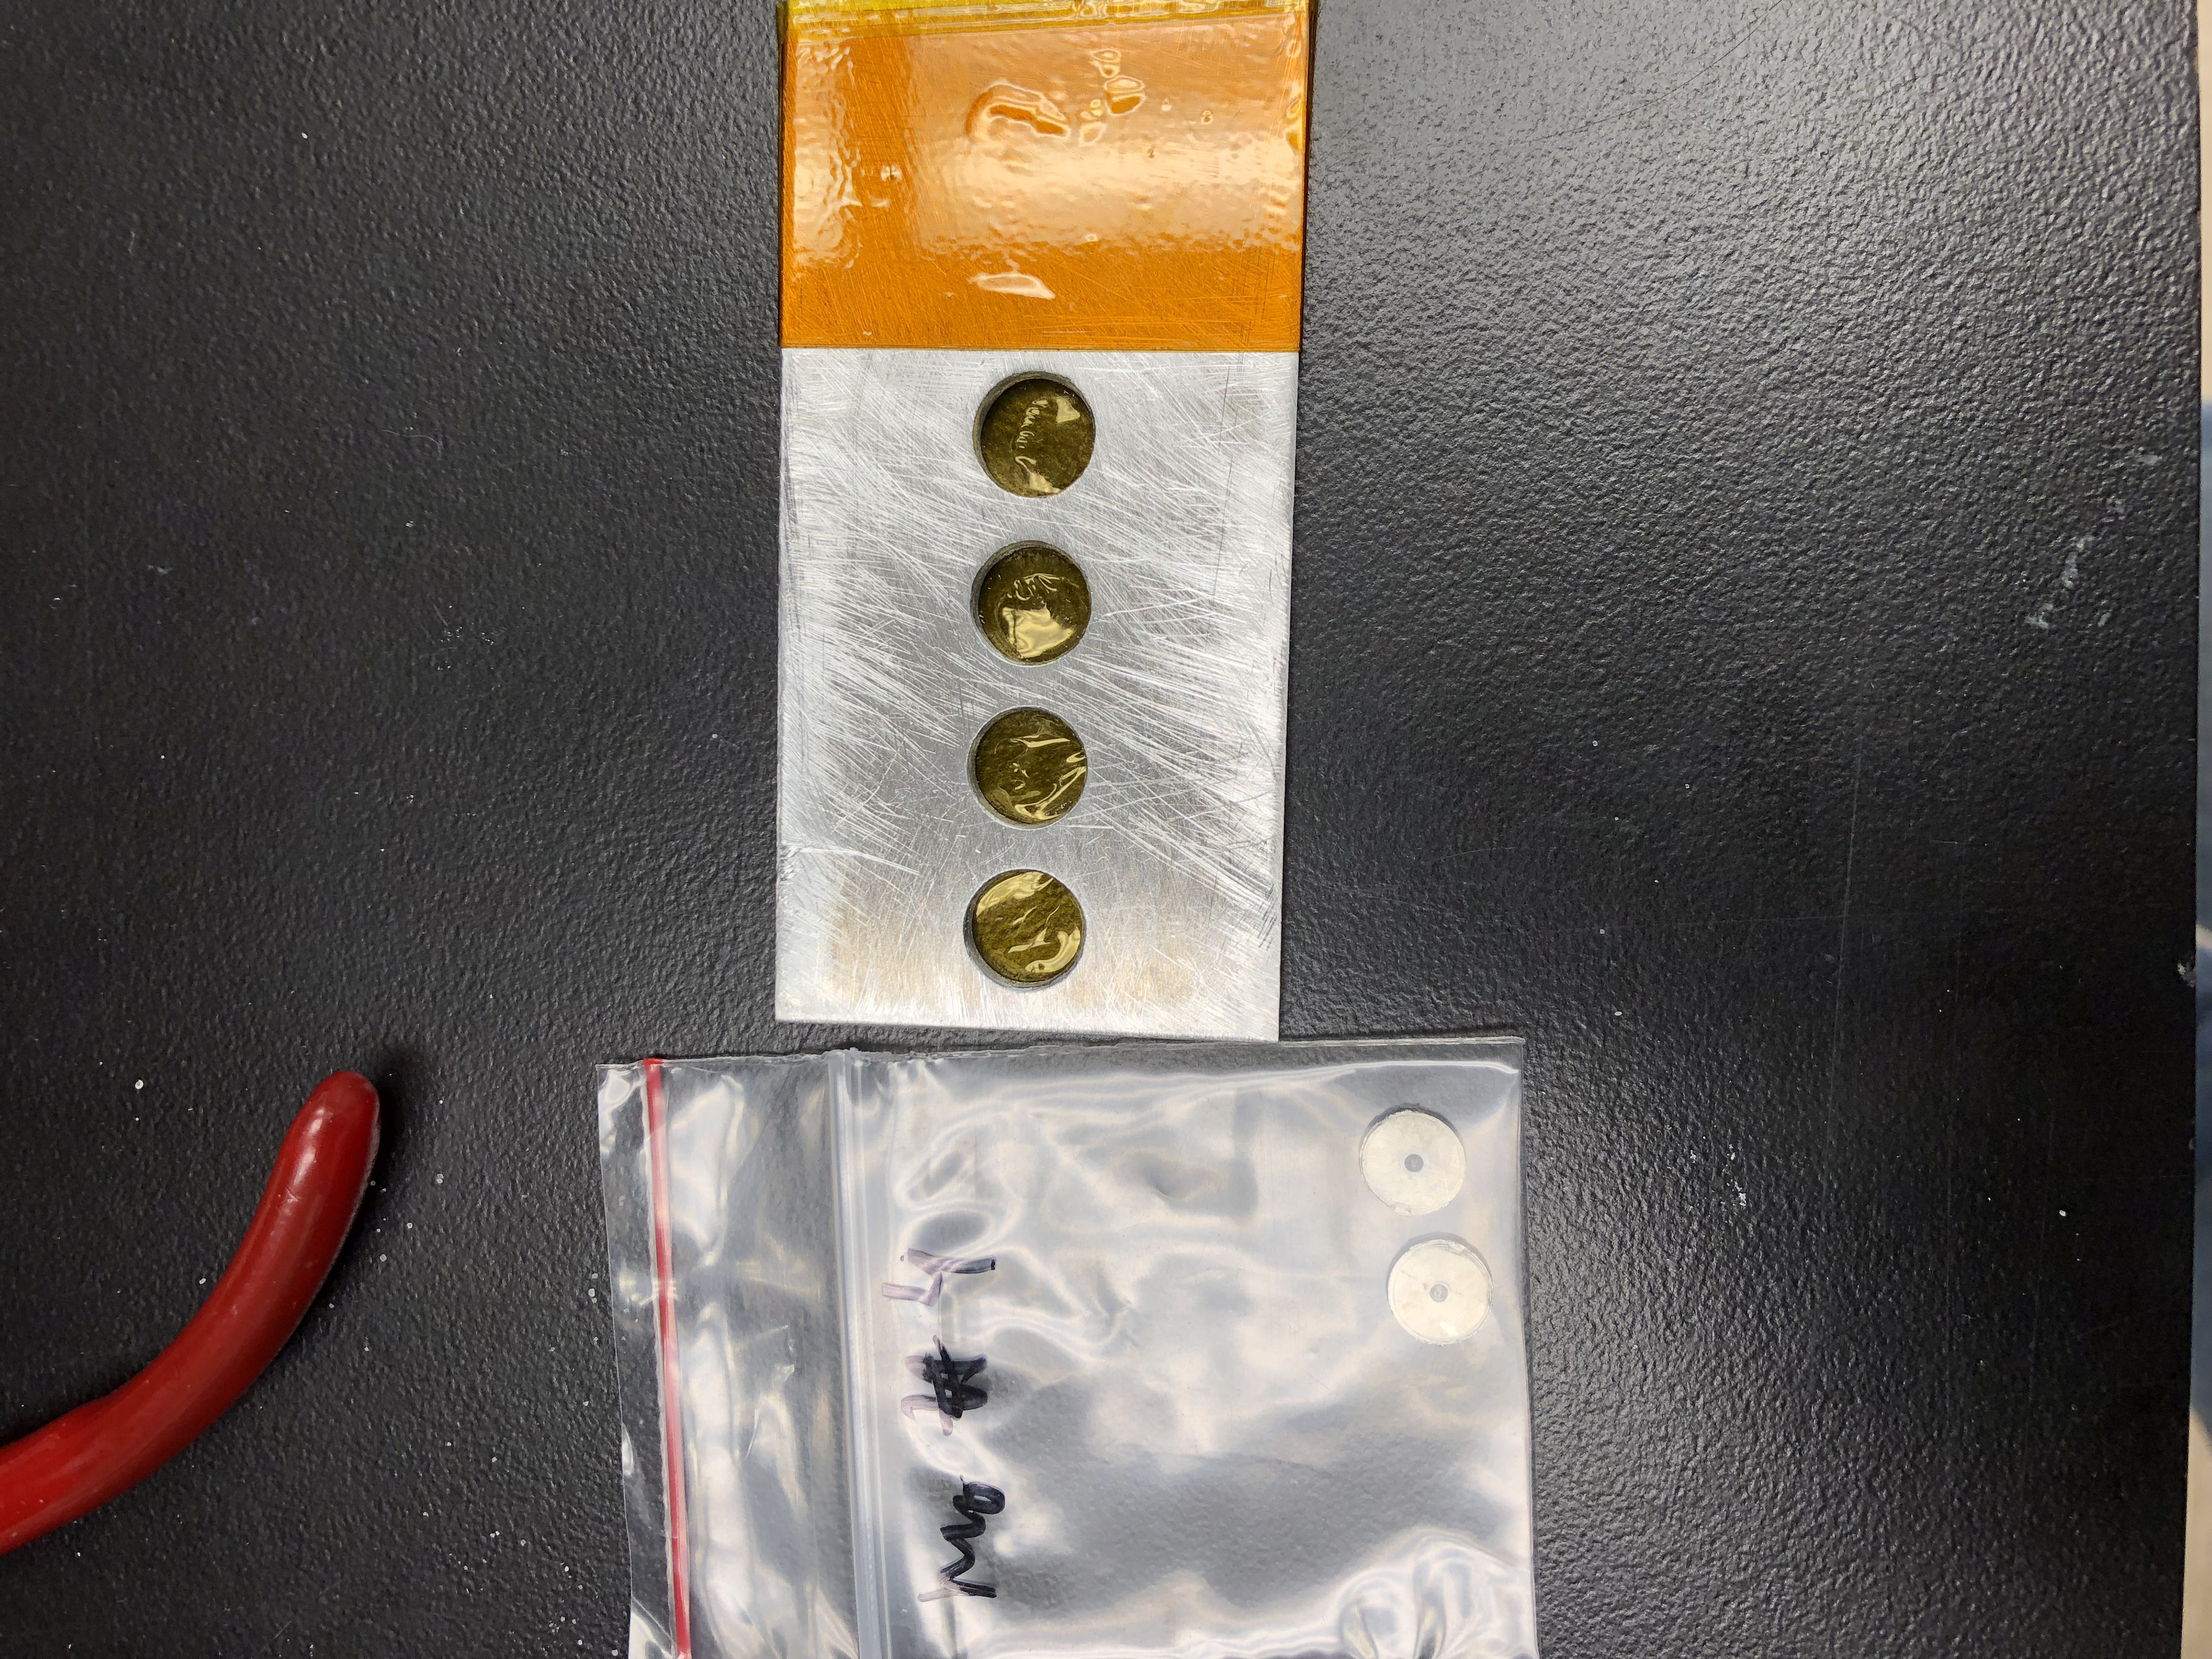
\includegraphics[clip=true,trim=5pt 1000pt 10pt 900pt,width=0.75\columnwidth,angle=90]{./figures/IMG_8840.JPG}
%  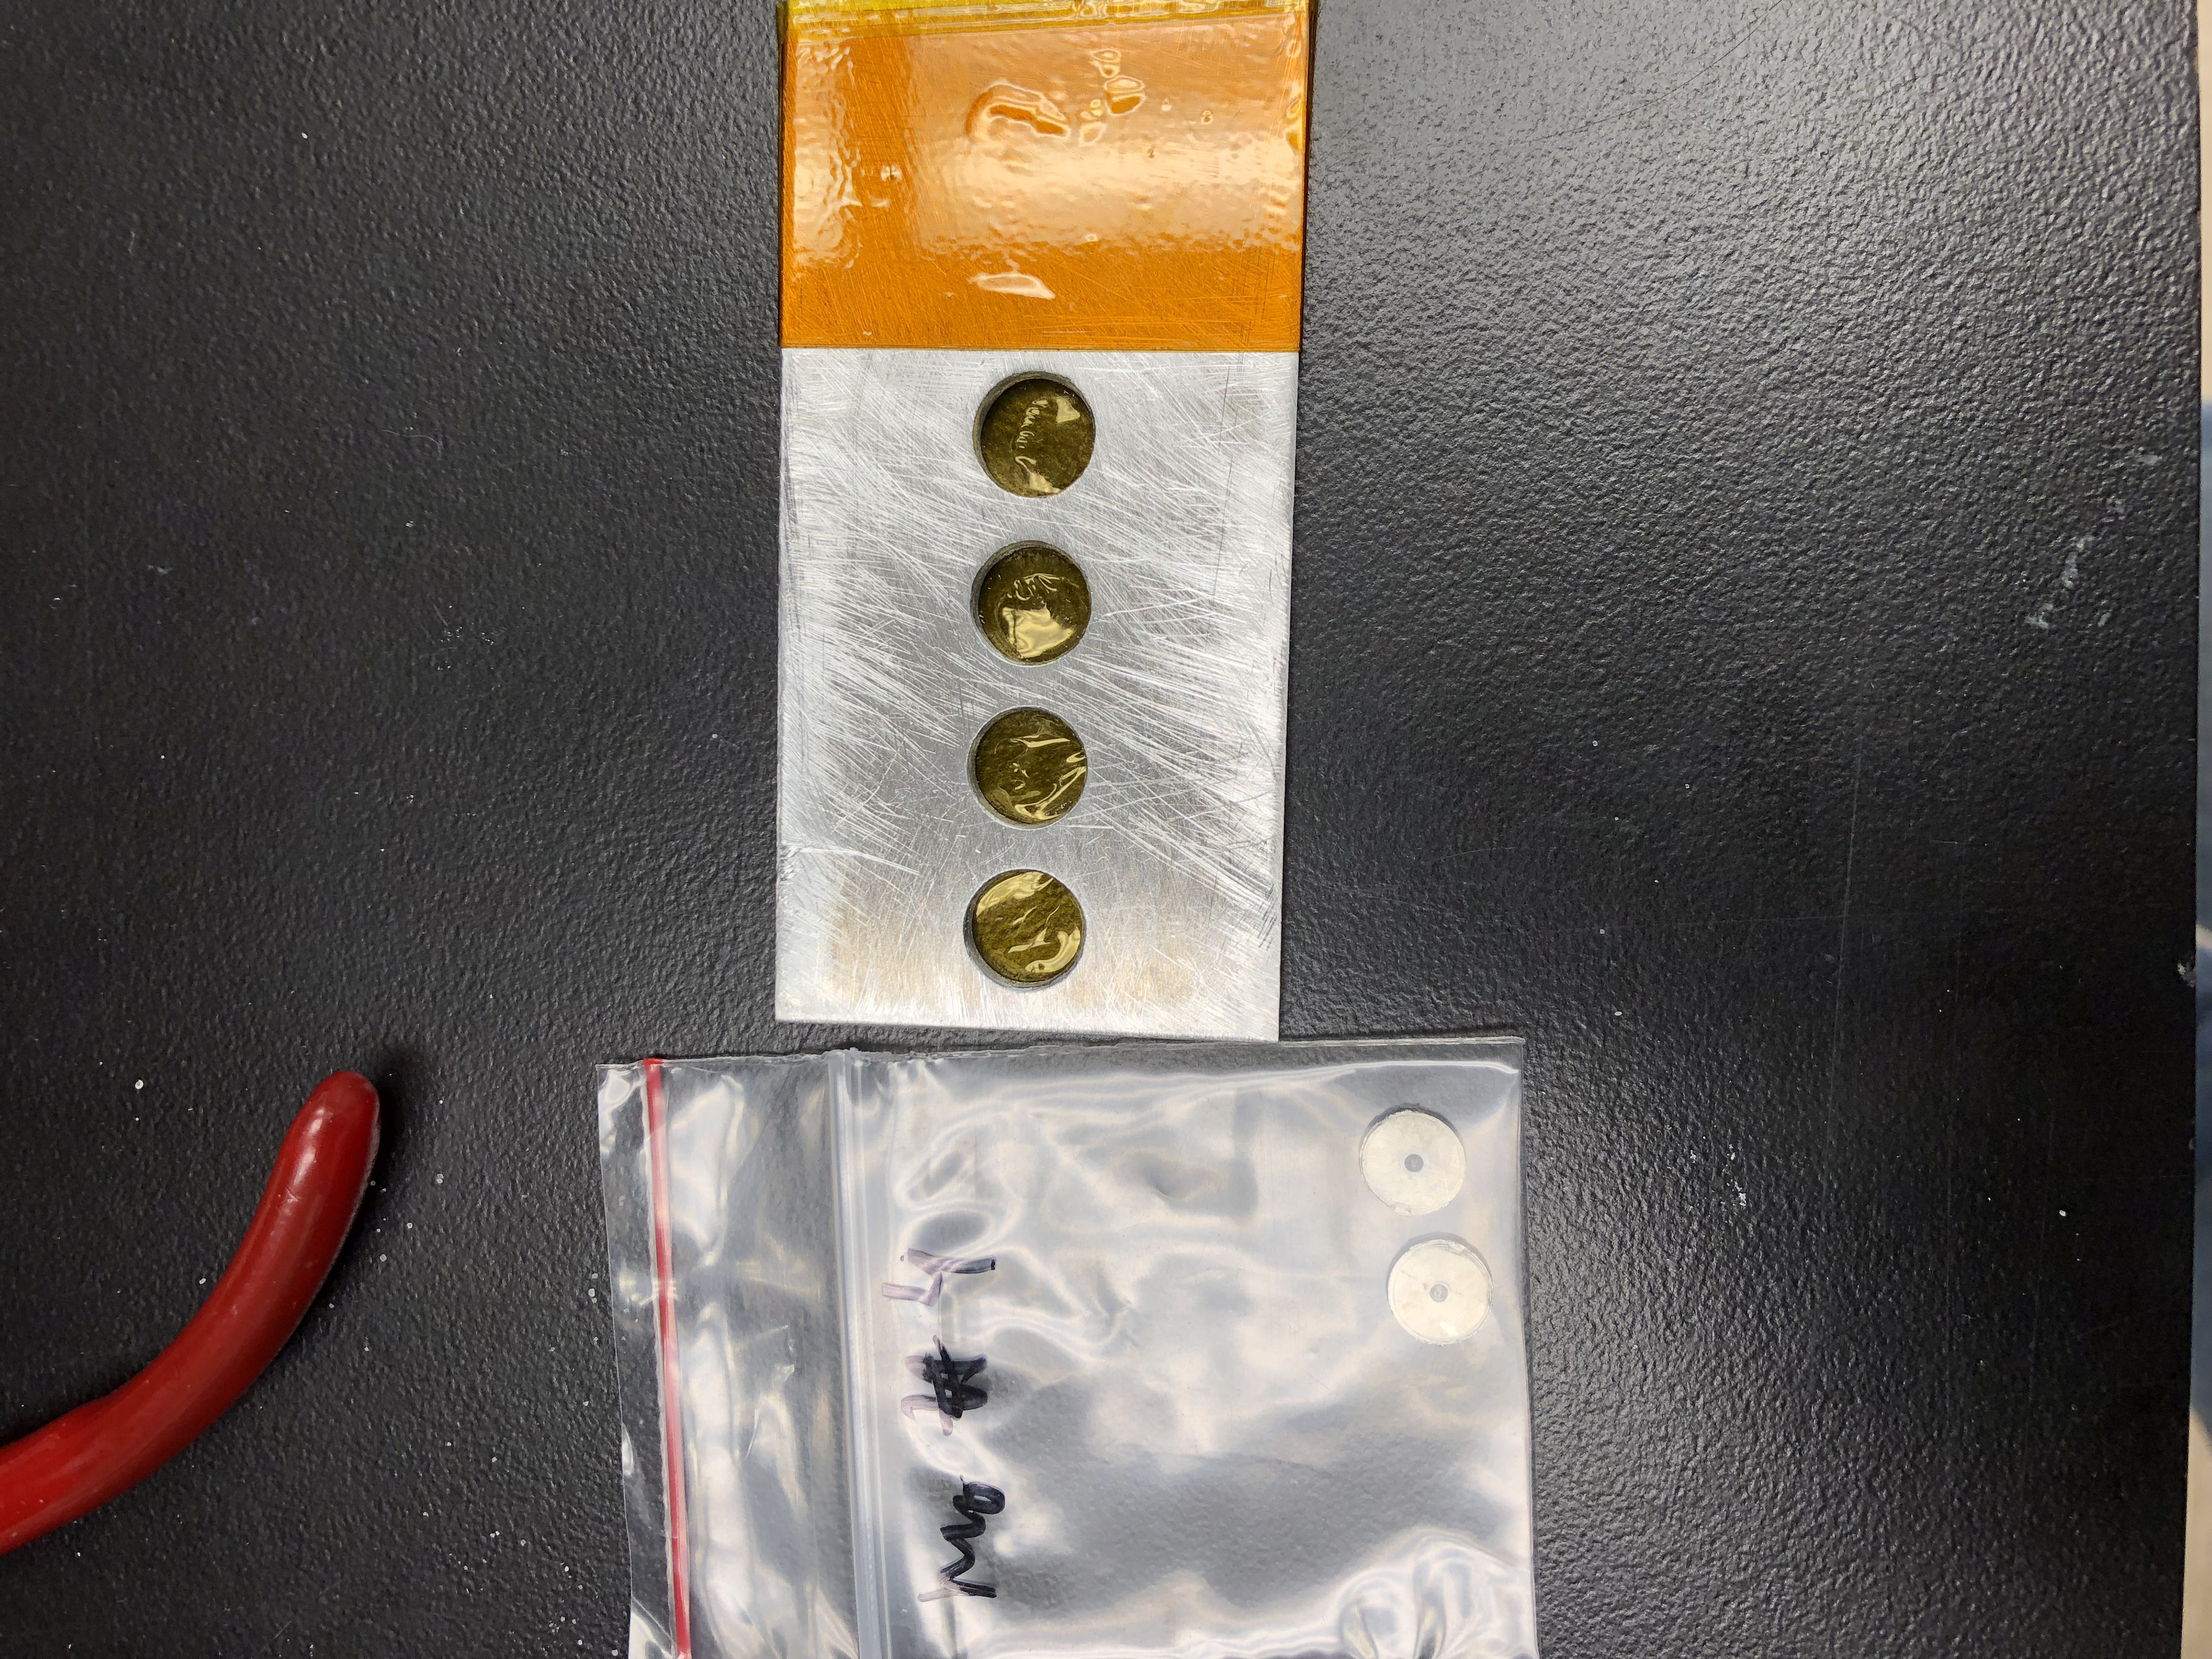
\includegraphics[width=0.75\columnwidth,angle=270]{./figures/IMG_8840.JPG}
 
\includegraphics[width=0.75\columnwidth]{./figures/ipf_beamline_schematic.png}
 % IMG_8840.JPG: 4032x3024 pixel, 72dpi, 142.24x106.68 cm, bb=0 0 4032 3024
 \caption{Schematic diagram of the LANSCE beamline at LANL. From the initial injectors, a proton beam is accelerated to 100\,MeV in a drift-tube linear accelerator, where it is diverted away to the IPF beamline, highlighted in red.}
 \label{fig:ipf_beamline_schematic}
\end{figure}

\begin{figure}
 \centering
%                                l   b      r    top
%  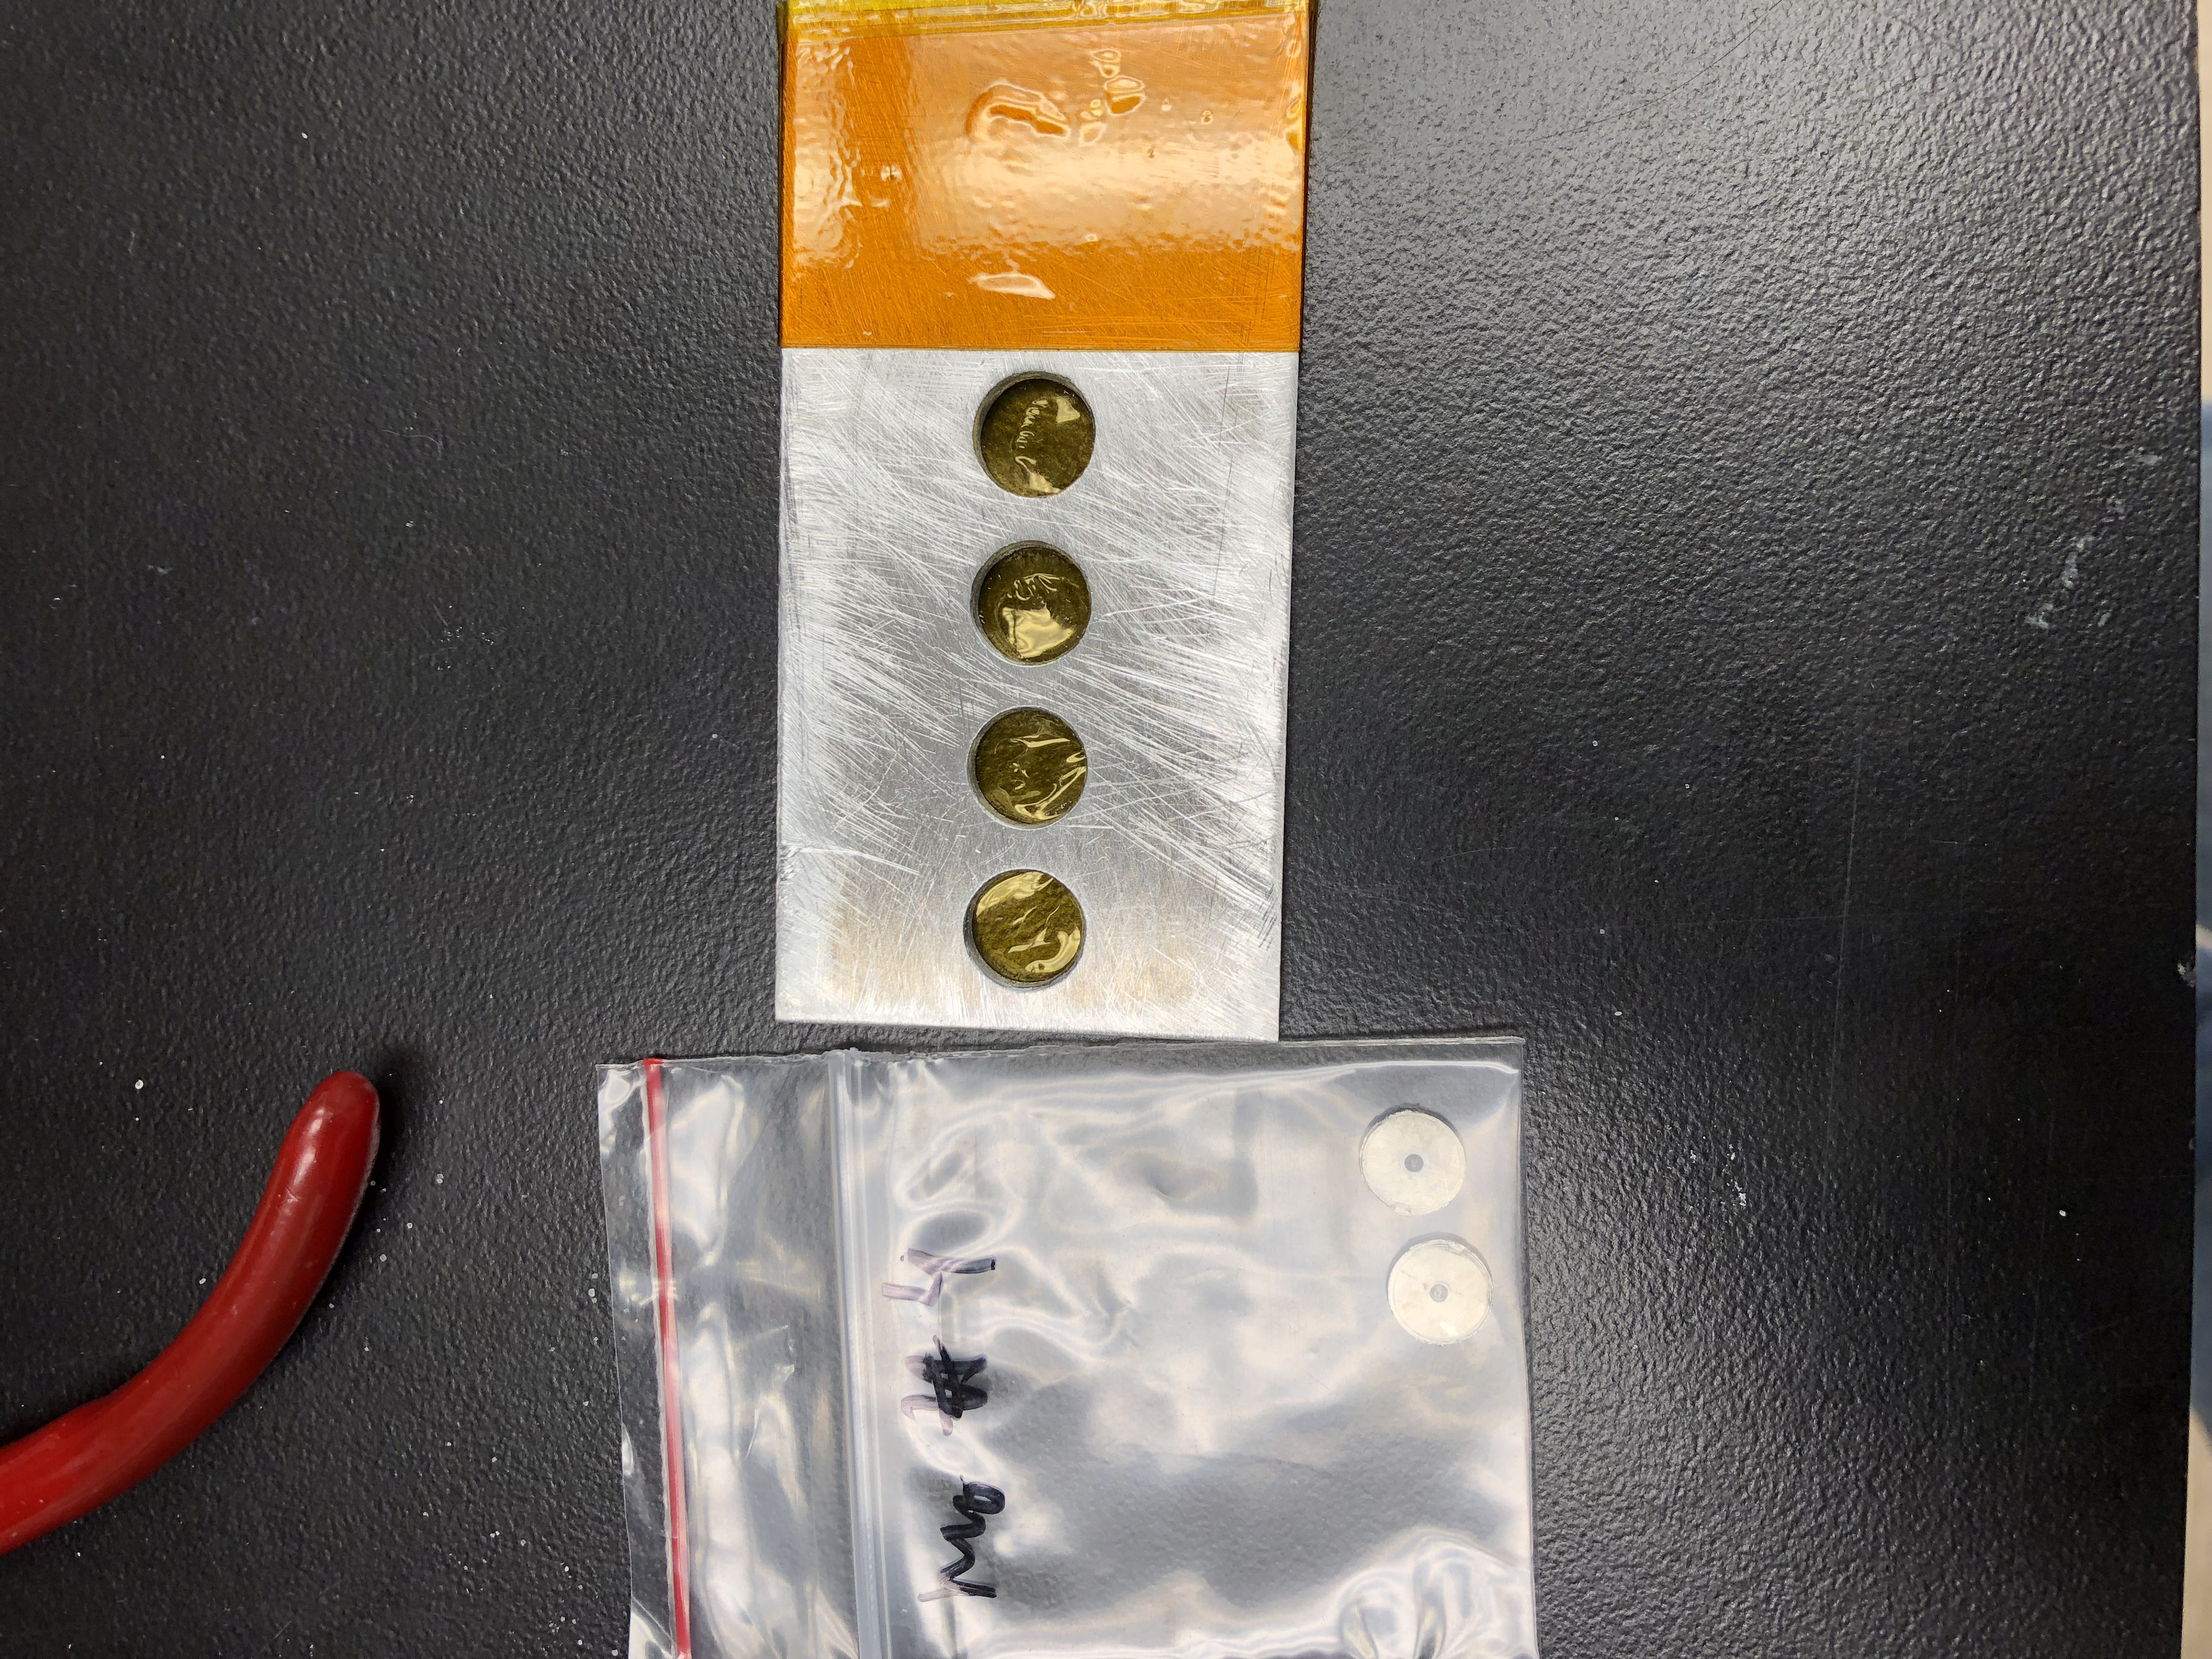
\includegraphics[clip=true,trim=5pt 1000pt 10pt 900pt,width=0.75\columnwidth,angle=90]{./figures/IMG_8840.JPG}
%  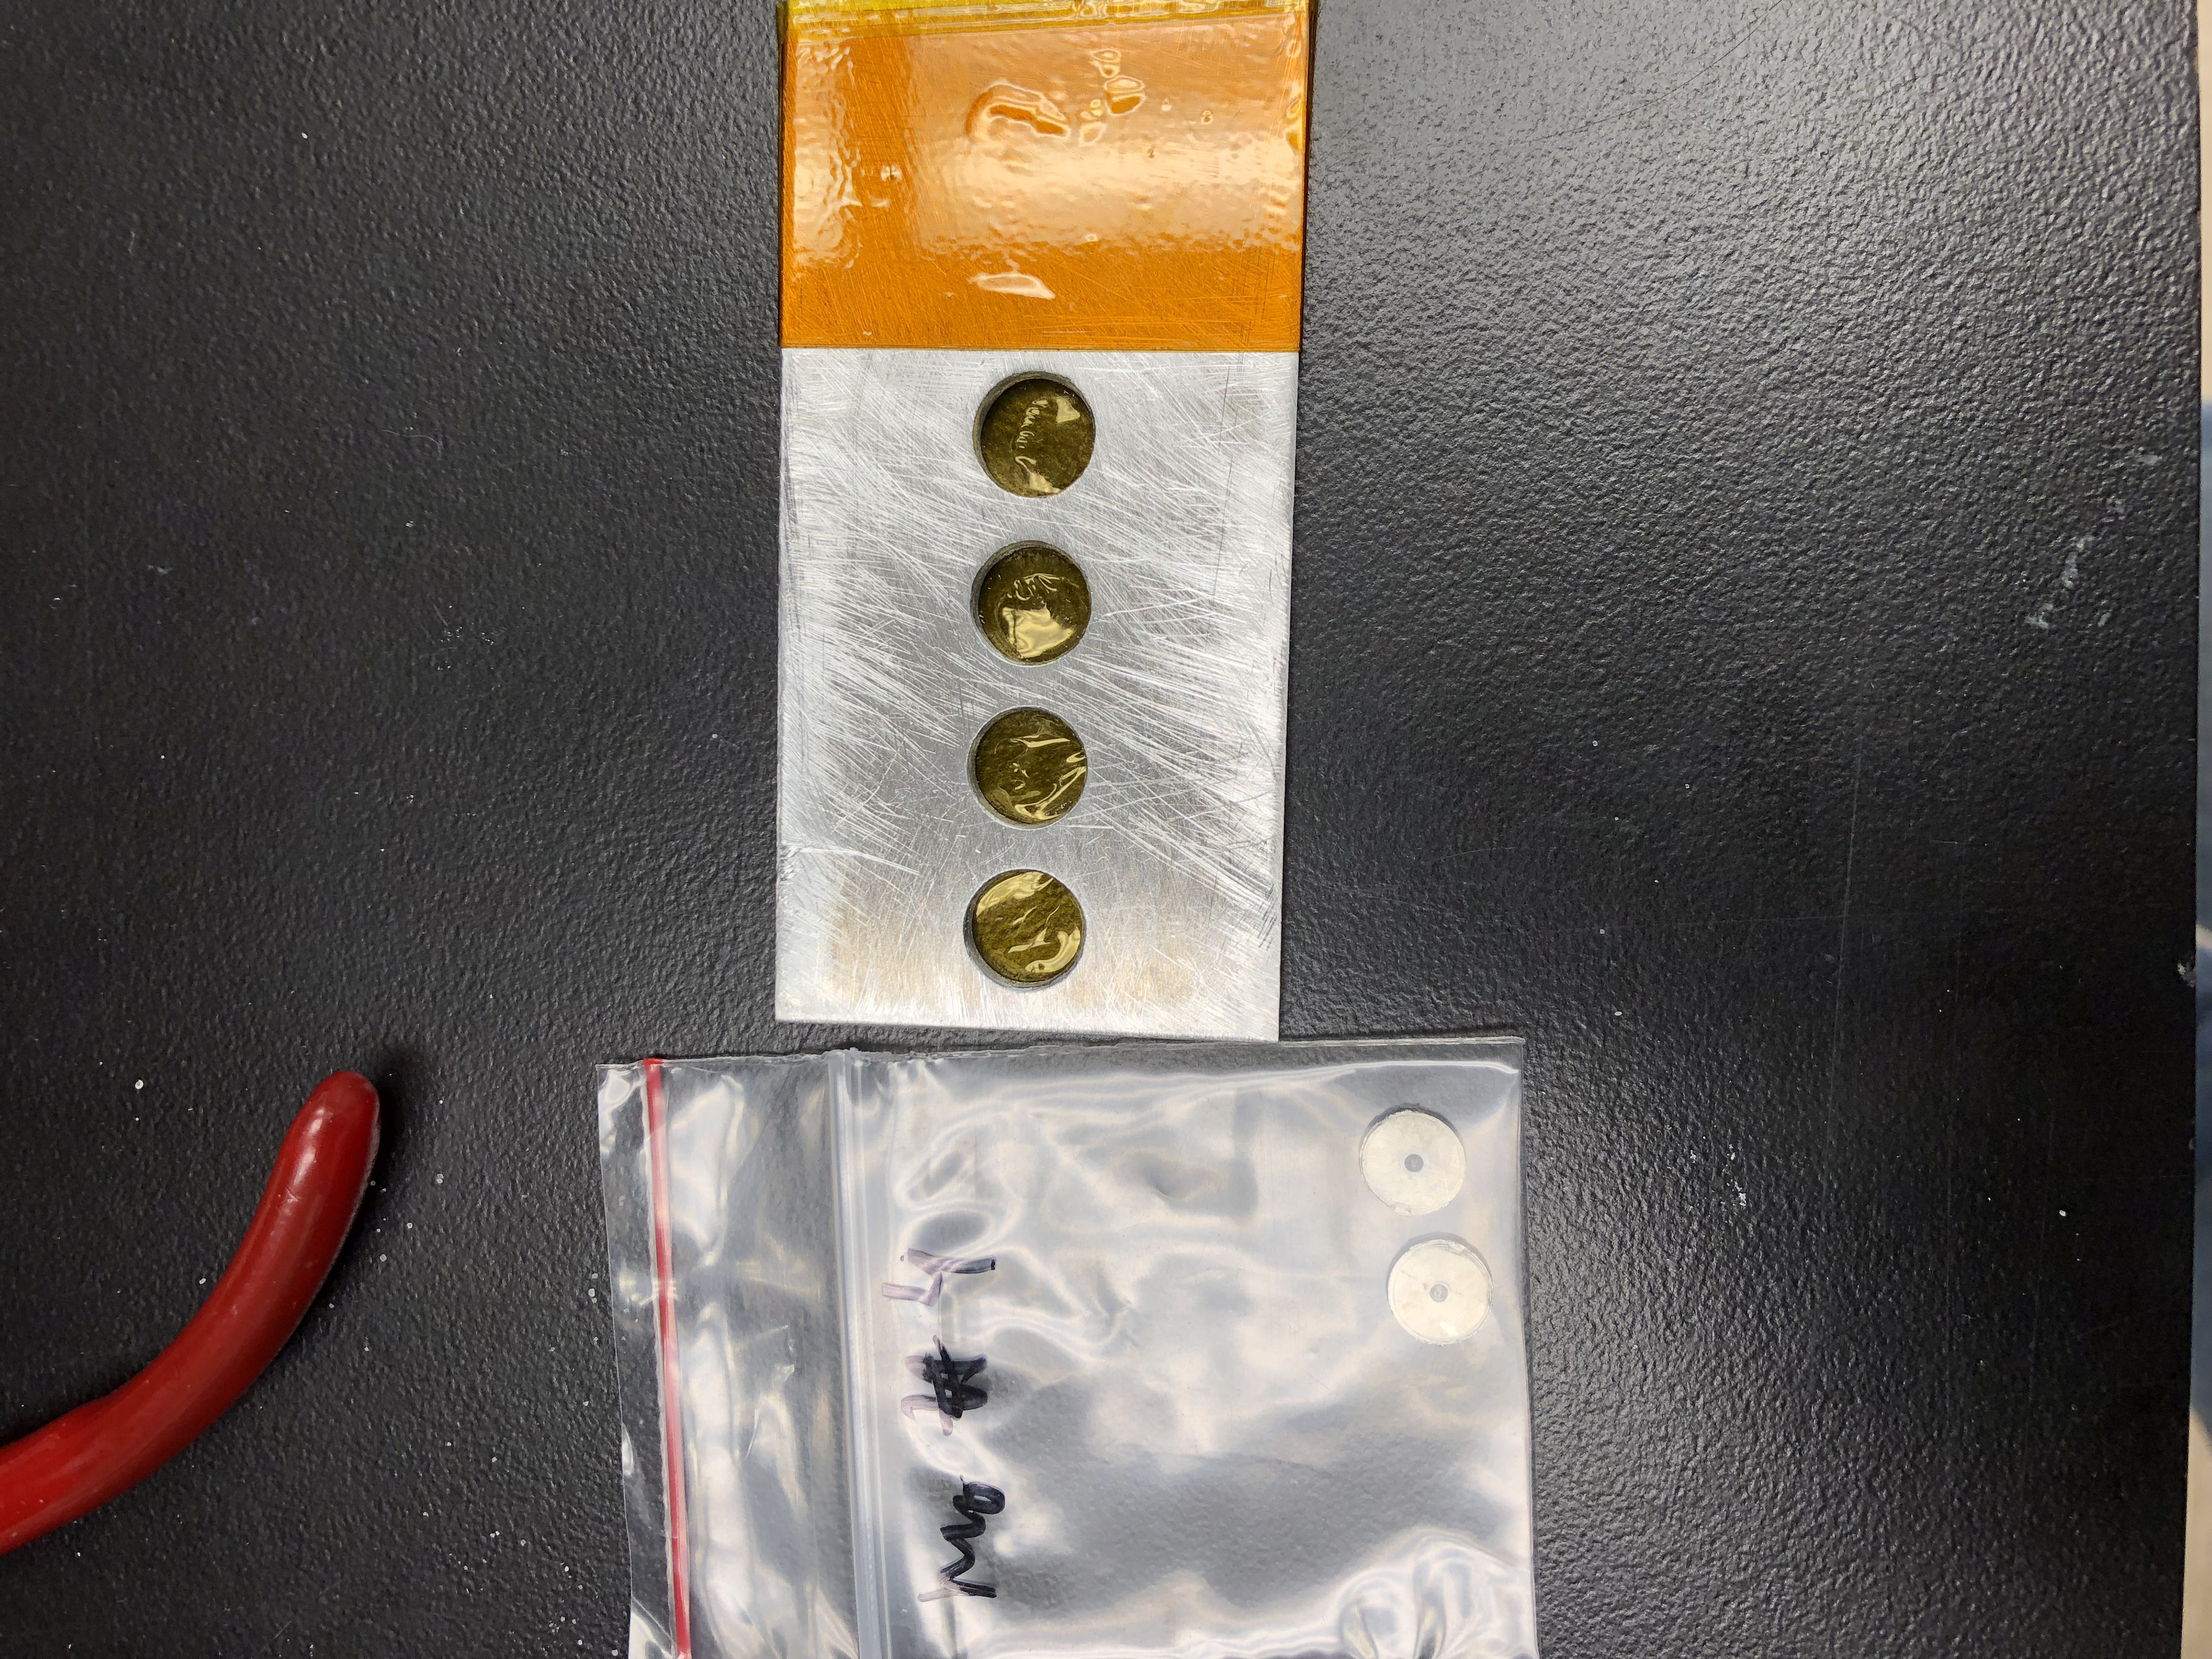
\includegraphics[width=0.75\columnwidth,angle=270]{./figures/IMG_8840.JPG}
 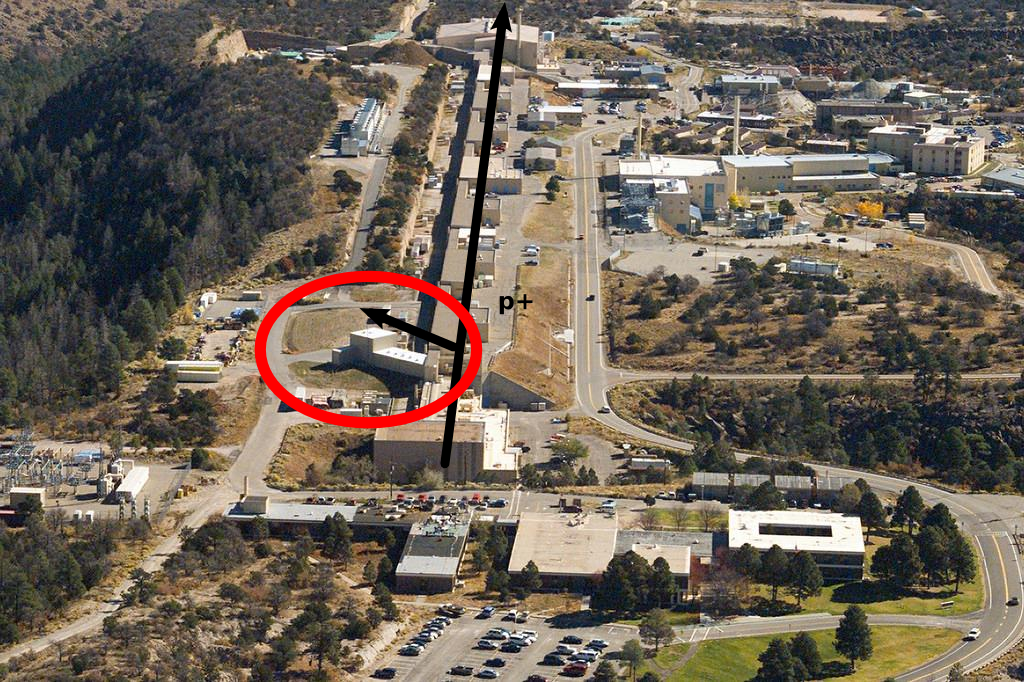
\includegraphics[width=0.75\columnwidth]{./figures/ipf_beamline_alternate.png}
 % IMG_8840.JPG: 4032x3024 pixel, 72dpi, 142.24x106.68 cm, bb=0 0 4032 3024
 \caption{Aerial photograph of the LANSCE beamline. Proton injectors are seen in the foreground building near the arrow's tail. The IPF beamline and operations facility is seen to the left of the main LANSCE beamline, circled in red.  The target box seen in \autoref{fig:target_stack} is lowered into the beamline here, via a hot cell.}
 \label{fig:ipf_beamline_alternate}
\end{figure}



\subsubsection{Radiation damage of materials}


% Following  tuning of the 100\,MeV proton beam into the IPF beamline, the current is measured immediately upstream of the target position using a pair of nondestructive inductive pickups.
% The final remaining step prior to loading the  target box for irradiation is to tune the beam optics and spatial profile.
% This is performed by loading a sheet of polyethylene (approximately 3\,mm thick) into the the IPF beamline, at the same location of the target box's beam entrance window. 
% This sheet acts as a beam profile monitor, and is irradiated with 5 \mmicro A-min of the proton beam.
As charged particles traverse a material, they transfer energy primarily through scattering reactions, leaving a damage trail along their path \cite{koutský2013radiation,krane1987introductory}.
The average energy transfer in a collision by an incident particle of energy $E$ and mass $m$, on a single atom
with mass $M$, is given by:
\begin{equation}
\langle T\rangle = \dfrac{1}{2}T_{max} = \dfrac{2mM}{\pp{m+M}^2}E
\end{equation}
For crystalline, metallic, and other ionic materials with a  well-defined bulk  lattice structure, if the energy transferred to an atom  is large enough, the atoms can  be knocked out of their lattice sites.
This displacement energy, $E_d$ , is typically about 25\,eV for most solid materials \cite{olander1990fundamental}. 
This displaced atom is referred to as the primary knock-on atom (PKA), and is now mobile and capable moving throughout the material, with energy $T$. 
If $T \ge E_d$, the PKA is free to collide with another atom in the lattice, transferring:
\begin{equation}
\langle T_2\rangle = \dfrac{1}{2}T_{max} = \dfrac{2mM}{\pp{m+M}^2}\langle T\rangle
\end{equation}
to the second atom. 
If $T_2 \ge E_d$, the PKA is free to collide with yet another atom, transferring:
\begin{equation}
\langle T_3\rangle = \dfrac{1}{2}T_{max} = \dfrac{2mM}{\pp{m+M}^2}\langle T_2\rangle
\end{equation}
% For crystalline, metallic, and other materials with a  well-defined bulk material lattice structure,  


This process keeps repeating, as long as $T_n \ge E_d$, producing a cascade of  atoms knocked out of their lattice sites, all of which are heavy charged ions, and will rapidly scatter in the nearby material. 
Each time an atom is knocked out of its lattice site, it produces a Frenkel pair --- the interstitial atom displaced from its lattice site, and a vacancy in its old lattice site \cite{olander1990fundamental,Pehl1978}. 
These are known as zero-dimensional defects in the material. 
During the cascade, all of the secondary interstitial displaced atoms may go on to knock out many other atoms themselves.
The cascade will continue on for $N_f$ total collisions, until the average energy of the cascade knock on particles is:
\begin{equation}
2E_d = \dfrac{T}{2^{N_f}}
\end{equation}
for an original incident radiation particle with energy $T$. 
This cascade will thus produce a total number of displaced particles, $\nu$, such that:
\begin{equation}
\nu = \dfrac{T}{2E_d}
\end{equation}
For the example of an original incident 1\,MeV proton, the proton may produce as many as
\begin{equation}
\nu = \dfrac{1\,MeV}{2\pp{25\,eV}} = 20,000\text{ displacements}
\end{equation}

All of the vacancy and interstitials formed by the cascade are extremely thermodynamically unstable, especially the interstitials, which are stuck in between lattice sites in the crystal lattice. 
To minimize the energy of the system, vacancies and interstitials diffuse from their primary site, and may recombine, annealing the damage caused by that pair \cite{shackelford2009introduction}. 
However, vacancies and interstitials may also diffuse towards like defects instead, linking to up form large three-dimensional void and precipitate cluster defects in the material, which also reduces the energy of the crystal system.
These defect clusters may easily be as large as 150\,\angstrom\ across. 
In addition, if the energy transfer in a PKA cascade is $\langle T \rangle \approx$ 5\,keV, cascades of such cluster defects may be formed nearly instantaneously, instead of single displacements \cite{Moll2000,Fourches2012a}.
It is worth pointing out that, in addition to the primary beam, secondary ionizing radiation may also cause material damage. 
However, due to the different interaction mechanisms for the different types of ionizing radiation, observed displacement cascades may have different energy thresholds.
Some typical threshold values for cascades are reported in \autoref{tab:cascade_thresholds} below.


% Please add the following required packages to your document preamble:
% \usepackage{booktabs}
\begin{table}
\centering
\caption{Displacement cascade approximate thresholds \cite{Moll2000}}
\label{tab:cascade_thresholds}
\begin{tabular}{@{}lll@{}}
\toprule
Incident Radiation Type & Single Displacements & Defect Clusters \\ \midrule
Charged Particles       & 0.2 keV/A            & 8 keV/A         \\
Neutrons                & 185 eV               & 5 keV           \\
Gammas                  & 1 MeV                & Not observed    \\ \bottomrule
\end{tabular}
\end{table}



While this gives a brief overview of radiation damage in ionic materials, for plastics and other amorphous polymer solids, a different damage  mechanism exists.
This is due to the fact that these types of material are dominated by covalent bonding.
In such materials, when atoms are sufficiently excited following scattering by ionizing radiation,  they are not displaced from their lattice position, but instead may have their electron bond pairs broken up.
This results in the original molecule  disintegrating, and potentially re-forming into one or more new, different molecules.
Thus, radiation damage in covalent materials results in chemical changes, as opposed to the physical changes seen in ionic materials.
Plastics and other polymers exist as a massive single macromolecule, formed by repeating chains of smaller molecules called monomers.
In the case of polymers, the extensive bond geometry in the overall molecule determines many of its properties and appearance, making such materials highly vulnerable to radiation damage \cite{Aframian1974}.




When polymer bonds are broken, free radicals are formed in the severed chain segments.
These free radicals are highly likely to propagate and terminate by reforming in new arrangements, which can be loosely lumped into three categories.
Cross-linking is the formation of new bonds between previously-separate chains.
This rearrangement produces a more rigid and brittle polymer with increased molecular mass, and is a common damage mechanism in softer polymers, such as silicones and polyethylenes.
Fragmentation is the termination of segments with broken bonds, leading to the formation of many separate short-chain polymers.
This rearrangement produces a softer, more fluid polymer with decreased molecular mass, and is a common damage mechanism in harder polymers, such as Lucite and synthetic rubbers.
Both cross-linking and fragmentation affect the materials properties of a polymer --- mechanical strength, solubility, and discoloration are commonly affected by these damage mechanisms. 
Finally, fragmented chain segments may polymerize to form completely new polymers than the original macromolecule, with a wide variety and chemical and physical properties \cite{Reichmanis1993}.


Of these materials properties, discoloration is one of the most commonly encountered radiation damage effects seen in the context of activation experiments.
Permanent discoloration occurs in polymers primarily due to heating effects from the beam.
Temporary, annealable discoloration is more common in activation experiments.
This variety is caused when residual free radicals become trapped in the polymer, and are unable to recombine and terminate.
Moreover, they are able to be reversed through annealing, disappearing as oxygen diffuses into the polymer, helping to terminate the residual free radicals.
This process will often occur at room temperature, but is greatly catalyzed when the polymer is heated \cite{international1999iaea,Davenas2002}.





\subsubsection{\label{sec:nb_profile_measurements}Beam profile measurements}

% \textred{Verify that we used polyethylene!!!}


Following  tuning of the 100\,MeV proton beam into the IPF beamline, the current is measured immediately upstream of the target position using a pair of nondestructive inductive pickups.
The final remaining step prior to loading the  target box for irradiation is to tune the beam optics and spatial profile.
This is performed by loading a sheet of polyethylene (approximately 3\,mm thick) into the the IPF beamline, at the same location of the target box's beam entrance window. 
This sheet acts as a beam profile monitor, and is irradiated with 5 \mmicro A-min of the proton beam.
Following exposure, the polyethylene monitor is withdrawn back into the IPF hot cell, where it is inspected to verify the shape and location of the beam profile.
These beam profile irradiations leave an annealable discoloration of the beam profile, which resembles a \enquote{burn mark}, and are observed to passively revert within 1--2 weeks.
The final pre-irradiation beam spot from the Nb(p.x) measurement is seen in  \autoref{fig:ipf_preexp_beam_spot}.
LANSCE accelerator operations staff use this feedback to fine-tune the beam, centering the beam spot upon the target stack and focusing it to ensure that it underfills the target foils.
This process of  optics tuning via polyethylene profile monitors is repeated until an acceptable beam profile is attained.
At this point, the target box is lowered into the beamline, and the irradiation commences.
 








\begin{figure}
 \centering
%                                l   b      r    top
%  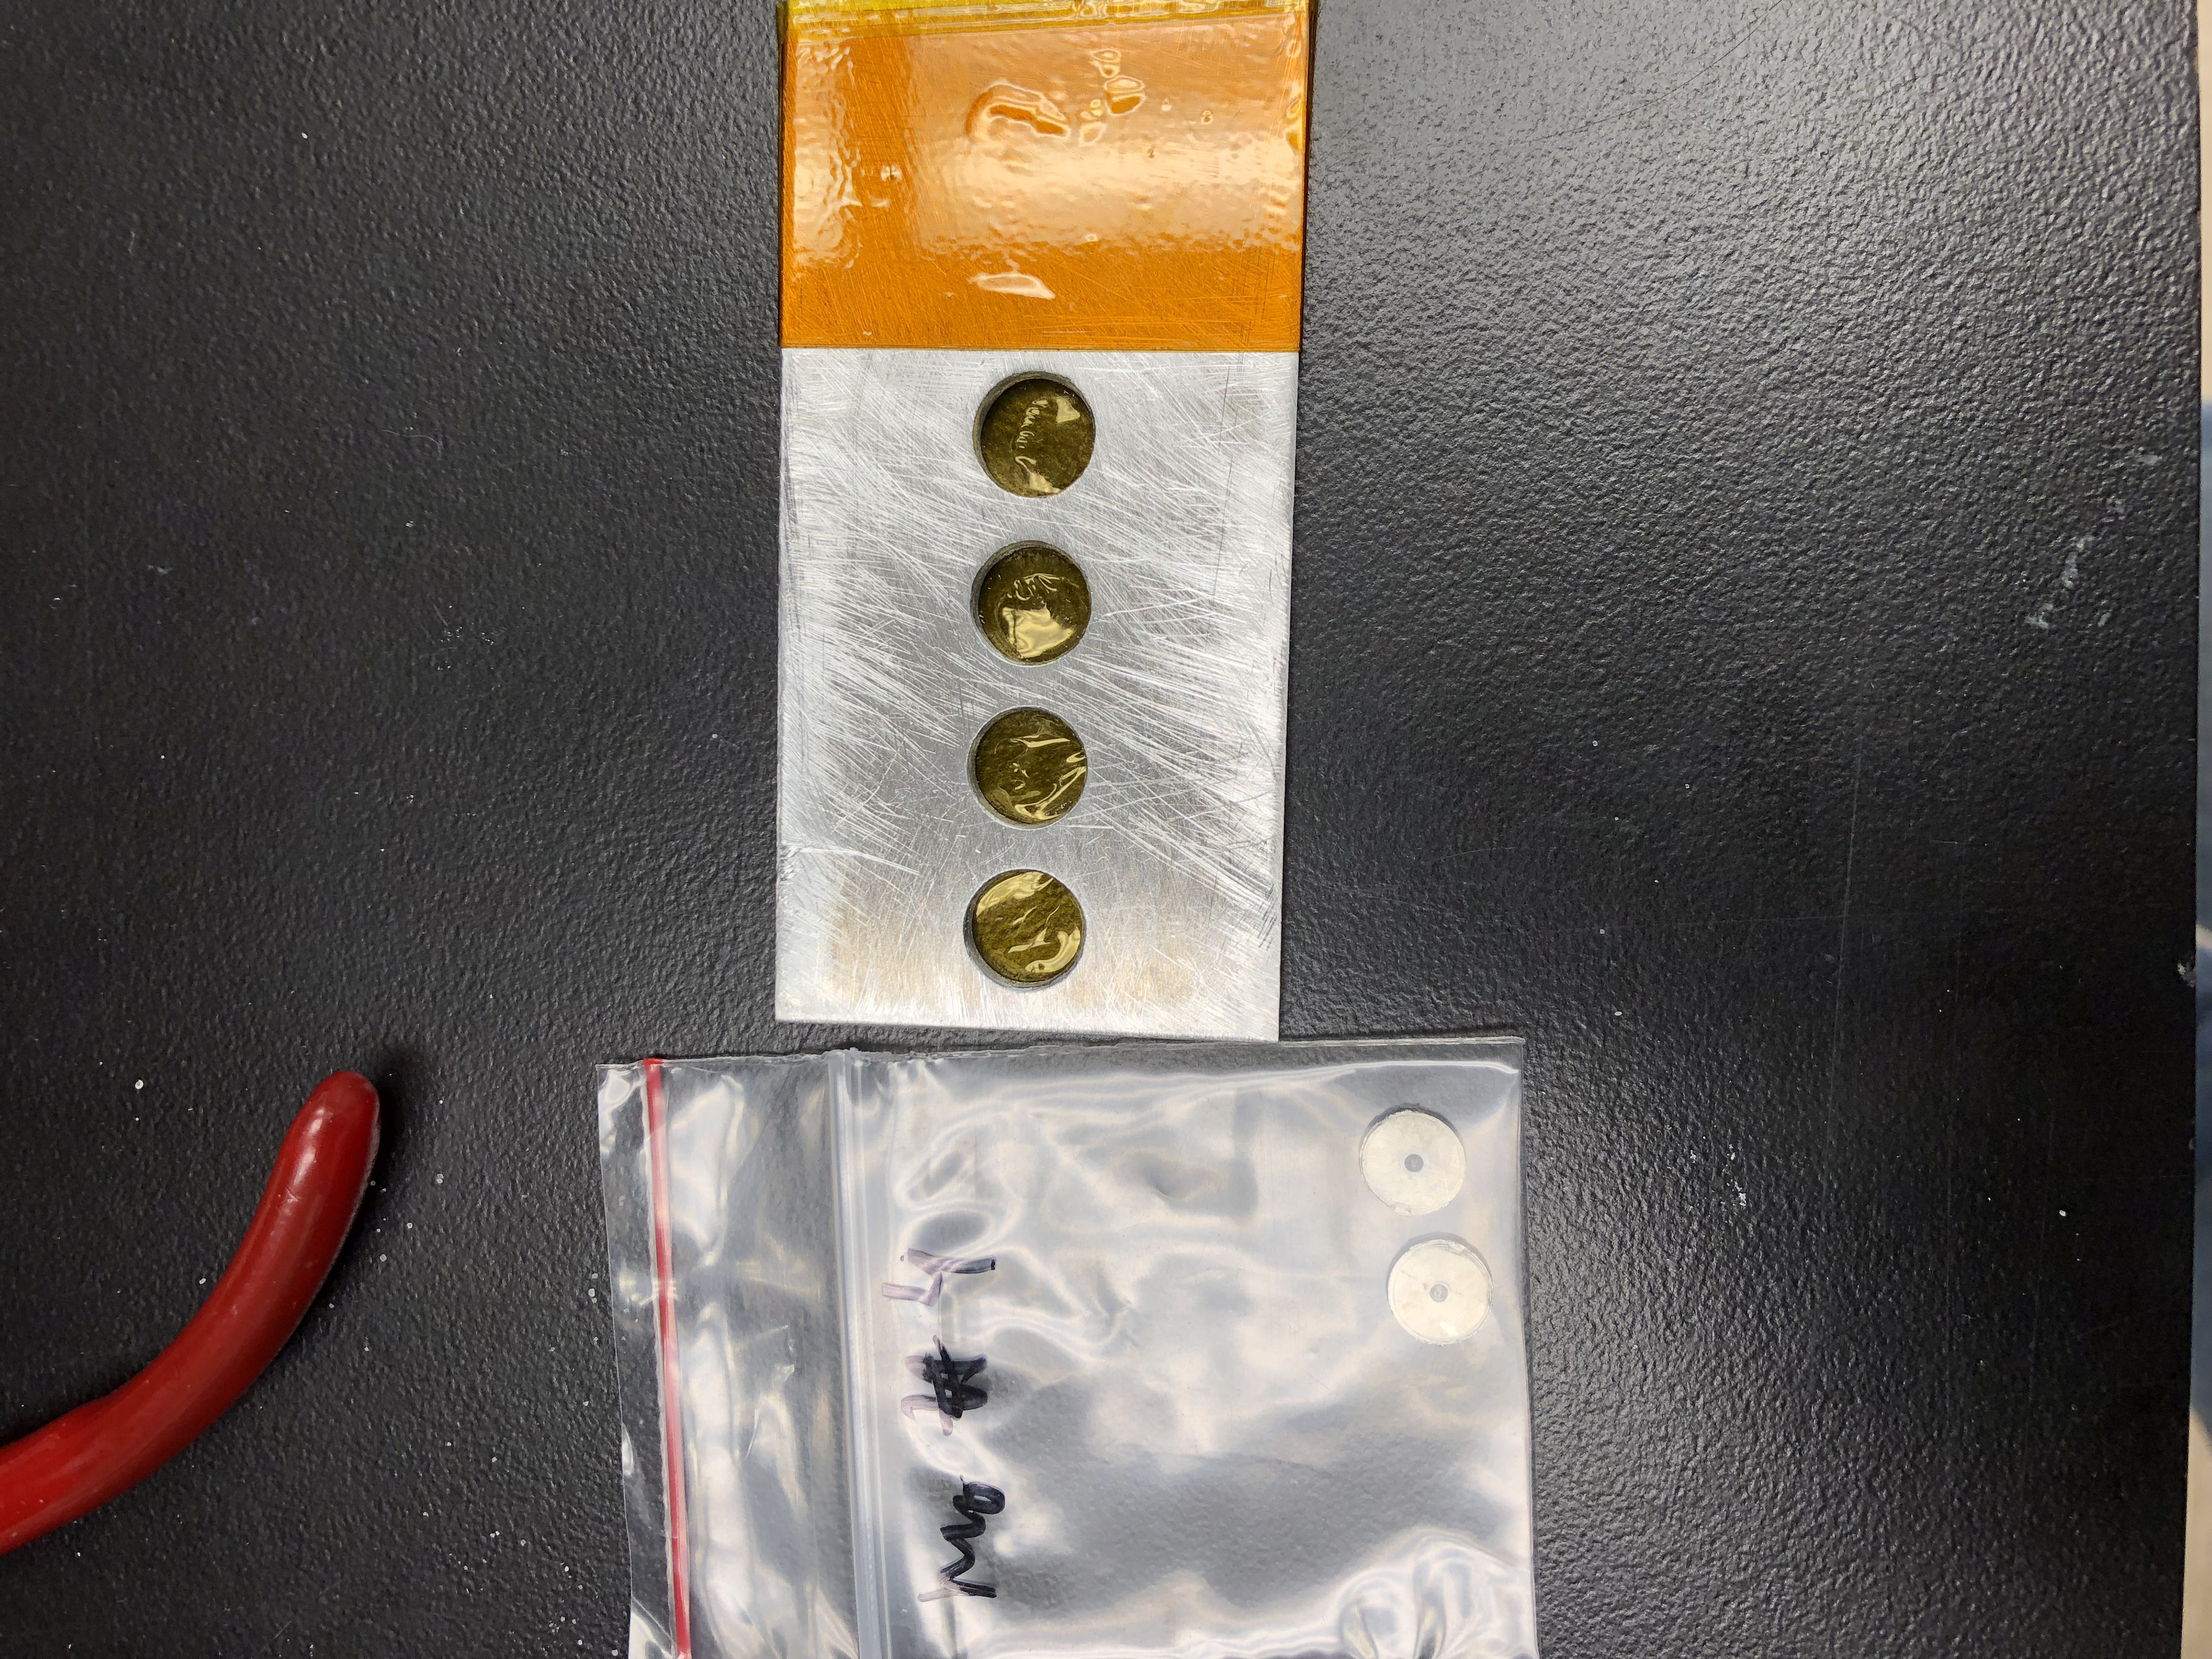
\includegraphics[clip=true,trim=5pt 1000pt 10pt 900pt,width=0.75\columnwidth,angle=90]{./figures/IMG_8840.JPG}
%  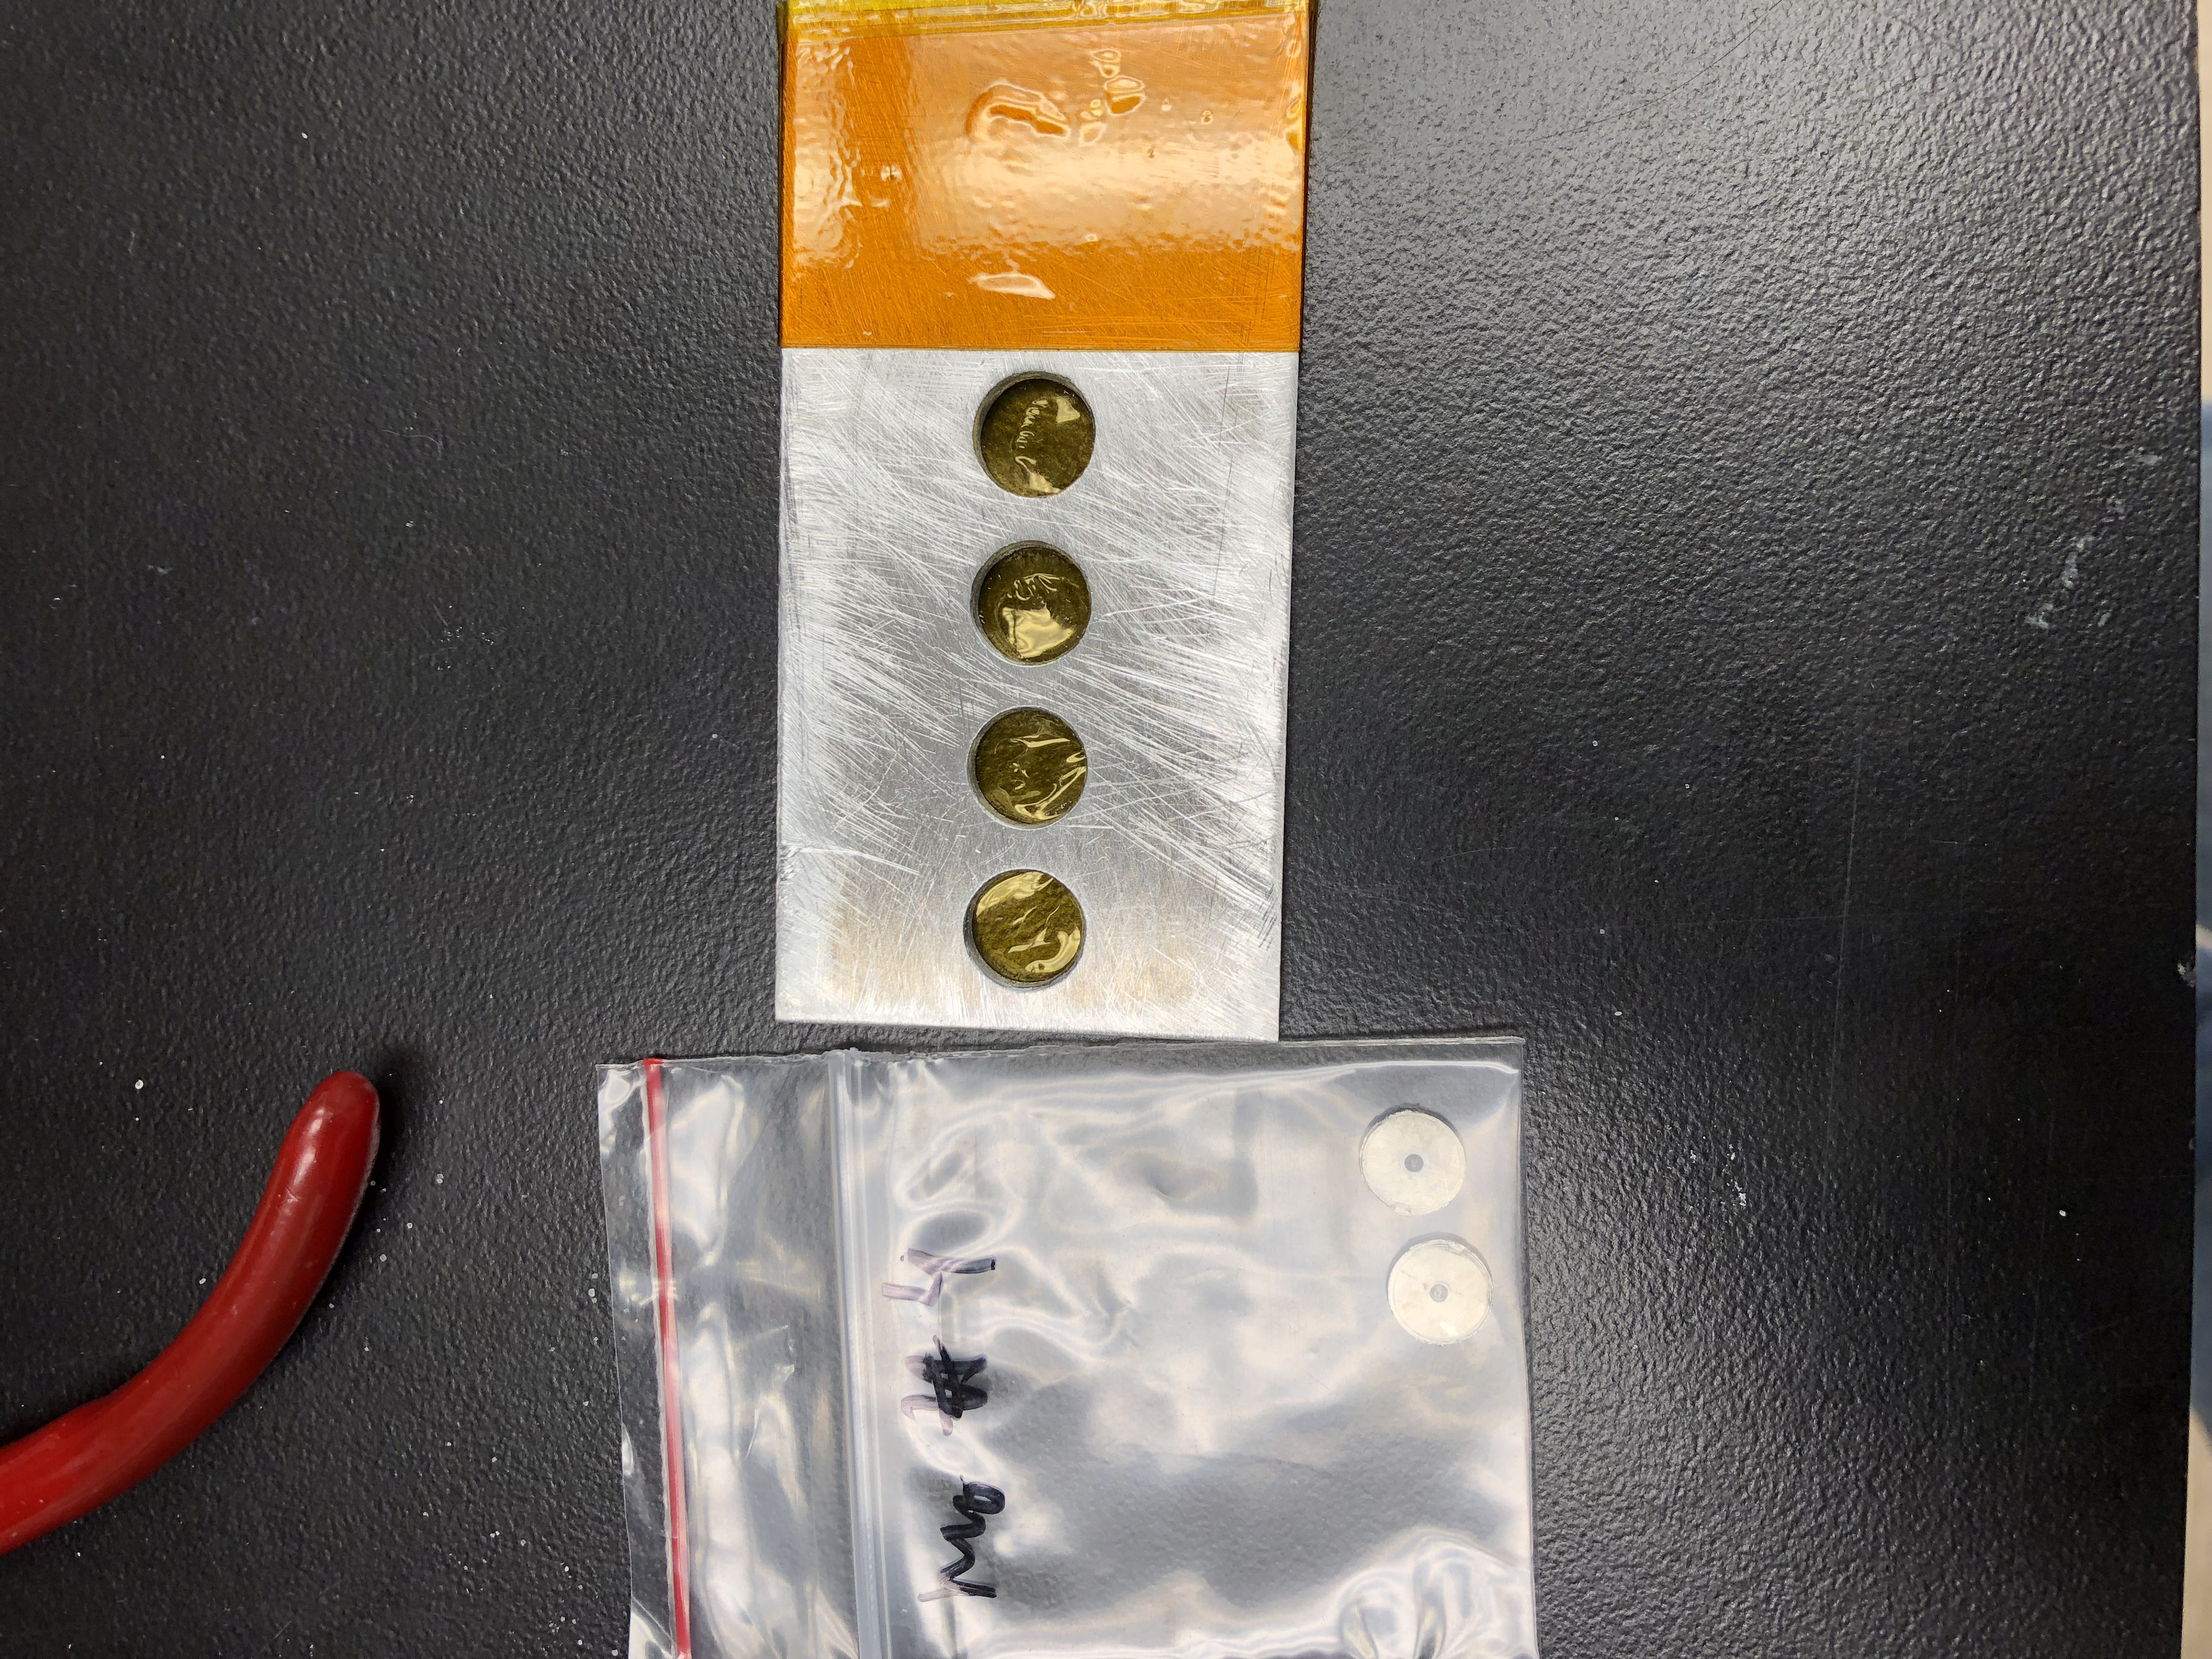
\includegraphics[width=0.75\columnwidth,angle=270]{./figures/IMG_8840.JPG}
 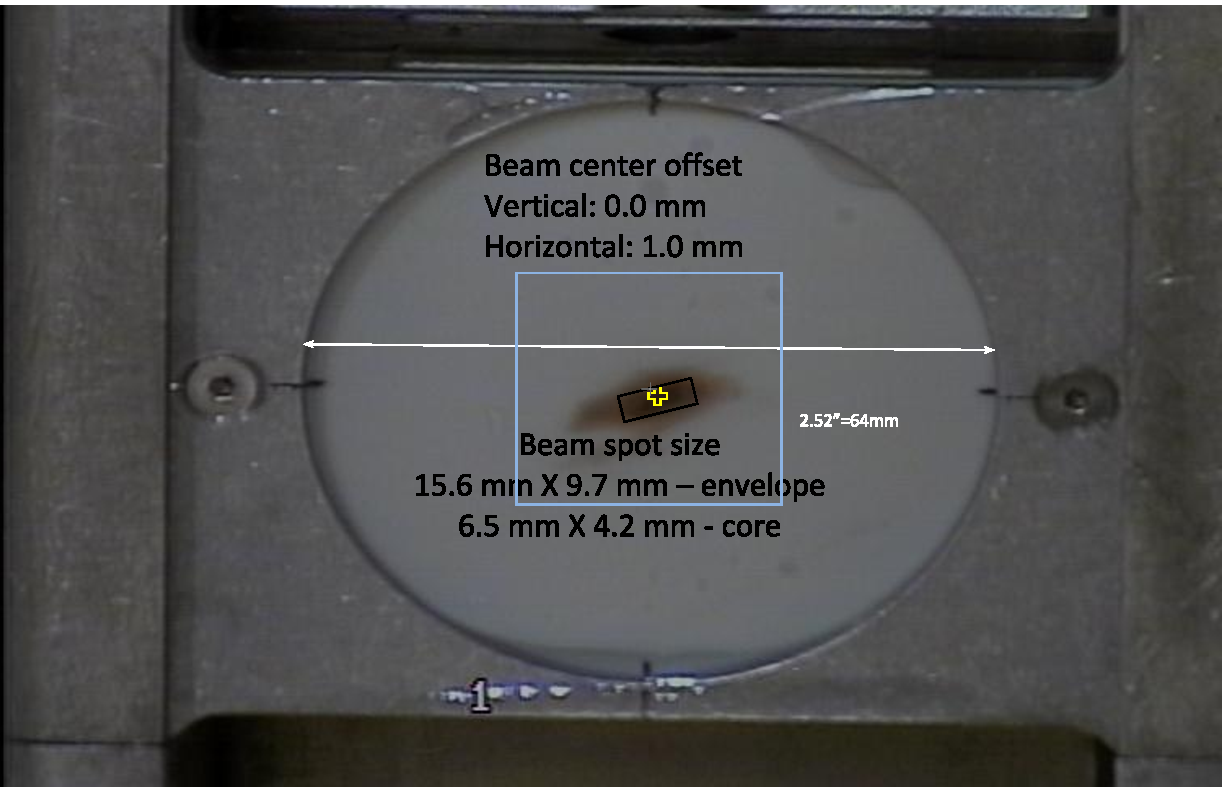
\includegraphics[width=0.75\columnwidth]{./figures/ipf_preexp_beam_spot-cropped.pdf}
 % IMG_8840.JPG: 4032x3024 pixel, 72dpi, 142.24x106.68 cm, bb=0 0 4032 3024
 \caption{Final beam spot profile for the IPF Nb(p.x) measurement. The 100\,MeV proton beam is confirmed to be centered on the target position, and is focused to underfill the 25$\times$25\,mm target foils.}
 \label{fig:ipf_preexp_beam_spot}
\end{figure}




This polyethylene beam profile monitor is useful for determining the beam profile incident upon the stack's beam entrance window.
However, the beam broadens as it traverses the target stack, with large-angle deflections (primarily in the aluminum degraders) from scattering of the beam.
To image the actual beam profile incident upon the first foil in the stack (Al-1), a 316 stainless steel foil (SS-6) is inserted upstream of Al-1 to serve as a beam profile monitor for the activation foils.
Likewise, another stainless steel profile monitor (SS-1) is inserted downstream of the last foil in the stack (Nb-6).
These stainless steel monitors are cut to the same length and width as the plastic frames used for mounting foils, and are characterized in \autoref{tab:stack_table}.





As described in \autoref{sec:target_design}, decay radiation emitted from the activated stainless steel foils were used to develop radiochromic film (Gafchromic EBT), revealing the spatial profile of the beam entering and exiting the stack.
Radiochromic films, such as Gafchromic EBT, come in multiple varieties, depending on the   dose range and the type of ionizing radiation desired to provide sensitivity to. 
In general, such films are commonly self-developing, containing a radiation-sensitive organic polymer dye as the active layer.
This dye, much like the polyethylene beam profile monitors, is damaged by ionizing radiation, with multiple free radicals initiated in the process.
These free radicals result in cross-linking, breaking of double bonds, and fragmentation of the dye polymer, which causes the damaged dye to undergo a large visible change in  color.
The intensity of this color change is often proportional to the dose received by the film, and is preferred to be energy-independent \cite{Azam1998}.
Many such films are sensitive to prolonged UV exposure, and will slowly develop if not kept in a  cool, dark environment, leading to systematic errors in observed dose.
The thin dye layer in most films is extremely sensitive, so care must be taken to avoid bending or deforming, which can make them insensitive to development when irradiated.
% Following exposure, the film may be scanned 
For reference, the Gafchromic EBT film used in this work is comprised of a pair of 25\,\mmicro m active layers containing the radiation-sensitive EBT emulsion dye, separated by a 3\,\mmicro m surface layer and sandwiched in between a pair of 97\,\mmicro m layers of clear polyester, acting as a supportive and protective backing. 






%  Move these first two commented sentences into PhD thesis.
% 
% % % 
% An accurate integrated proton current is one of the most important factors in performing high-fidelity cross section measurements.
% At the time of this work, the nondestructive beam current monitors in the LANSCE-IPF beamline had a  resolution of 100 nAh.
% For a low-current irradiation such as this work, where a nominal fluence of 200 nAh is desired, additional fluence sensitivity is thus needed to accurately normalize quantified EoB activities into cross sections.


The radiochromic films developed by the SS-6 and SS-1 stainless steel beam profile monitors are seen in \autoref{fig:gafchromic_nb}.
In addition, extra aluminum monitor foils mounted on  plastic frames are superimposed behind each film.
It is clear from the upstream (SS-6) film that the proton beam profile was consistent with that seen in the final pre-irradiation beam spot check of  \autoref{fig:ipf_preexp_beam_spot}.
The downstream (SS-1) film  reveals that the beam was not completely attenuated,  
% in the target stack
and clearly displays the  broadening expected due to scattering in the target stack. 
More importantly, the beam profiles in both films appears to be completely contained within the 25$\times$25\,mm activation foils, including the beam envelope.
If the beam were to be misaligned on the foils, or were to have sufficiently broadened such that it greatly overfilled the foils, the activation foils would be exposed to only a fraction of the total beam current.
If  fluence measurements are purely taken from an external  current monitor (such as an inductive pickup upstream of a target, or an electrically-isolated target in a Faraday cup), the  fraction of current which misses the foils will not be detected.
This leads to reporting a false, larger  fluence, which will cause all cross sections to be erroneously reported with a reduced magnitude.
Thus, it is for this  reason that having monitor foils at each energy position builds confidence in reported cross sections, as they serve to screen for systematic errors such as this.
However, profile monitors play a vital role in the detection of lost beam fluence when monitor foils are unavailable. 
% Additionally, 







Since the color change developed by irradiation is proportional to the dose deposited in the film, the optical density of the film may be used to measure dose.
In clinical external-beam radiation therapy, these films are commonly used in quality assurance  to map and verify  the dose contours for therapeutic gamma-ray fields.
However, the dose sensitivity of these films is often greater than the ability to be visually distinguished beyond simple qualitative inspection.
As a result, following exposure, the film may be digitized using any flatbed scanner.
Image analysis may be thus used to measure the optical density profile as a surrogate for dose or beam intensity profiles.
The optical density is often fit to a curve of the form
\begin{equation}
d_x\pp{D} = a + \dfrac{b}{D-c}
\end{equation}
where $d_x\pp{D}$ is the optical density of exposed radiochromic film in scanner color channel $x$ at dose $D$, and $a$, $b$, and $c$ are calibration parameters.
Using a standard irradiation source (commonly a collimated \ce{^{60}Co} source), a calibration curve can thus be measured to convert optical density into an absolute dose.
This is most common in clinical and quality assurance applications.
In addition, modern radiochromic films are often designed such that the characteristic exposure curve for the active layer dye differs between the red, green, and blue color channels, offering even further enhanced sensitivity to dose \cite{bushberg2011essential,Andre2011,David2012}.





However, for cases where an absolute dose is not necessary, the optical density can still be used for a qualitative measure of relative beam intensity, or relative dose.
Using the image analysis code  ImageJ-2.0.0,  profiles of the total optical density were extracted for both the SS-1 and SS-6 radiochromic films \cite{Rueden2017}.
These are seen in \autoref{fig:gafchromic_nb_profiles}, as relative beam intensity profiles along the major and minor axis of each film.
As seen visually, for both axes, the peak beam intensity drops from SS-6 to SS-1, as the proton fluence is clearly broadened by scattering reactions in the target stack.
% As seen visually, there is a clear broadening of the beam spot in the rear of the target stack.
Along the major (\enquote{horizontal}) axis, the FWHM of the beam profile broadens from 0.679\,cm to 1.039\,cm, and along the minor (\enquote{vertical}) axis, the FWHM of the beam profile broadens from 0.453\,cm to 0.902\,cm.
In addition, the centroid position of the minor axis appears to shift by approximately 0.19\,cm between the front and rear of the stack. 
The measured beam profiles were fit using a Gaussian model with linear background, to aid in comparing the widths of each profile.
The Gaussian model does well to fit the beam profiles overall, though it overestimates the peak height for a given Gaussian width.
This is likely due to the fact that the beam itself has an intrinsic spatial width before any interactions with the target stack; this leads to more broadening of the beam envelope than of its core.

    



\begin{figure}
    \centering
    \subfloat{
        \centering
%         \includegraphics[width=\columnwidth]{./figures/Capture.PNG}
        \hspace{-5pt}\subfigimg[width=0.5\textwidth]{a)}{./figures/DOC013119-cropped.pdf}{80}
%         \caption{ Decay curve for the isomeric transition of \ce{^{115m}In}.}
         %         \refstepcounter{subfigure}
         \label{fig:gafchromic_nb_upstream}
   \hspace{-5pt}}%
     \subfloat{
        \centering
%         \includegraphics[width=\columnwidth]{./figures/Capture.PNG}
%         \includegraphics[scale=0.6]{./figures/391keV_curve2.png}
        \subfigimg[width=0.5\textwidth]{b)}{./figures/DOC013118-cropped.pdf}{80}
%         \caption{ Decay curve for the isomeric transition of \ce{^{113m}In}.}
         %         \refstepcounter{subfigure}
         \label{fig:gafchromic_nb_downstream}
   \hspace{-5pt}}%
    \caption{Radiochromic films for the IPF Nb(p,x) measurement, developed by the stainless steel beam profile monitors in (a) the front of the stack (SS-6) and (b) the rear of the stack (SS-1). An unused Al monitor foils is aligned behind each film, confirming that both the beam core and envelope underfilled the activation foils.}
     \label{fig:gafchromic_nb}
\end{figure}




\begin{figure}
    \centering
    \subfloat{
        \centering
%         \includegraphics[width=\textwidth]{./figures/target2.png}
        \subfigimg[width=0.496\textwidth]{a)}{./figures/horz_ipf_beam_profile.pdf}{150}
%         \caption{Decay curve for the $\beta^-$ decay of \ce{^{116}In}.}
        %         \refstepcounter{subfigure}
%          \label{fig:54Mn}
%
%         \includegraphics[width=\columnwidth]{./figures/Capture.PNG}
        \subfigimg[width=0.496\textwidth]{b)}{./figures/vert_ipf_beam_profile.pdf}{50}
%         \caption{ Decay curve for the $\beta^+$ decay of \ce{^{64}Cu}.}
%         \refstepcounter{subfigure} 
%         \label{fig:55Co}
   \hspace{-10pt}}%
    \caption{Relative beam intensity profiles for the radiochromic films seen in \autoref{fig:gafchromic_nb}. The intensity profiles were analyzed using ImageJ along (a) the major axis and (b) minor axis of each beam spot. }
     \label{fig:gafchromic_nb_profiles}
\end{figure}




\subsubsection{Target preparation}

As described in \autoref{sec:target_design}, all activation  foils in this work were   tightly sealed into \enquote{packets} using two pieces of  3M 5413-Series Kapton polyimide film tape.
The sealed foils were then mounted over the hollow center of a 1.575 mm-thick plastic frame.
This gives each foil a fixed, rigid, position, preventing it from shifting out of alignment as the target stack is lowered into the beamline.
In addition, the hollow center is cut out such that the plastic frame does not degrade and scatter the beam at each foil position.
% to minimize the 
One \ce{^{nat}Al}, one \ce{^{nat}Cu}, and one \ce{^{nat}Nb} mounted foil were bundled together using baling wire for each energy position.
One such bundle is seen in \autoref{fig:IMG_1969}, illustrating how the three foils of each bundle are aligned with each other.
This is primarily to maintain a comparable area of exposed foil at each energy position, in the case of significant beam spot broadening.
These foil packet bundles were lowered into the beamline by inserting them into a  water-cooled production target box.
After sealing the target box, it is inserted into the IPF hot cell, seen in \autoref{fig:IMG_1984}. 
In the hot cell, robotic manipulators are used to attach a mounting frame to the top of the target box.
The frame is used to mount the target box onto a motorized track, which extends  below the hot cell, and is used to lower the target box  approximately 12\,m into its position in the IPF beamline.
Following irradiation, the track raises the target box back into the hot cell, where it is detached and opened via manipulators.
Foil removal is performed in the hot cell via the manipulators, as the target box becomes highly activated with short-lived Al activation products, which makes manual handling hazardous.
The foil bundles are removed using the baling wire loop \enquote{handles}, and  removed from the hot cell via a pass-through, for decontamination and transfer to the counting lab.




\begin{figure}
 \centering
%                                l   b      r    top
%  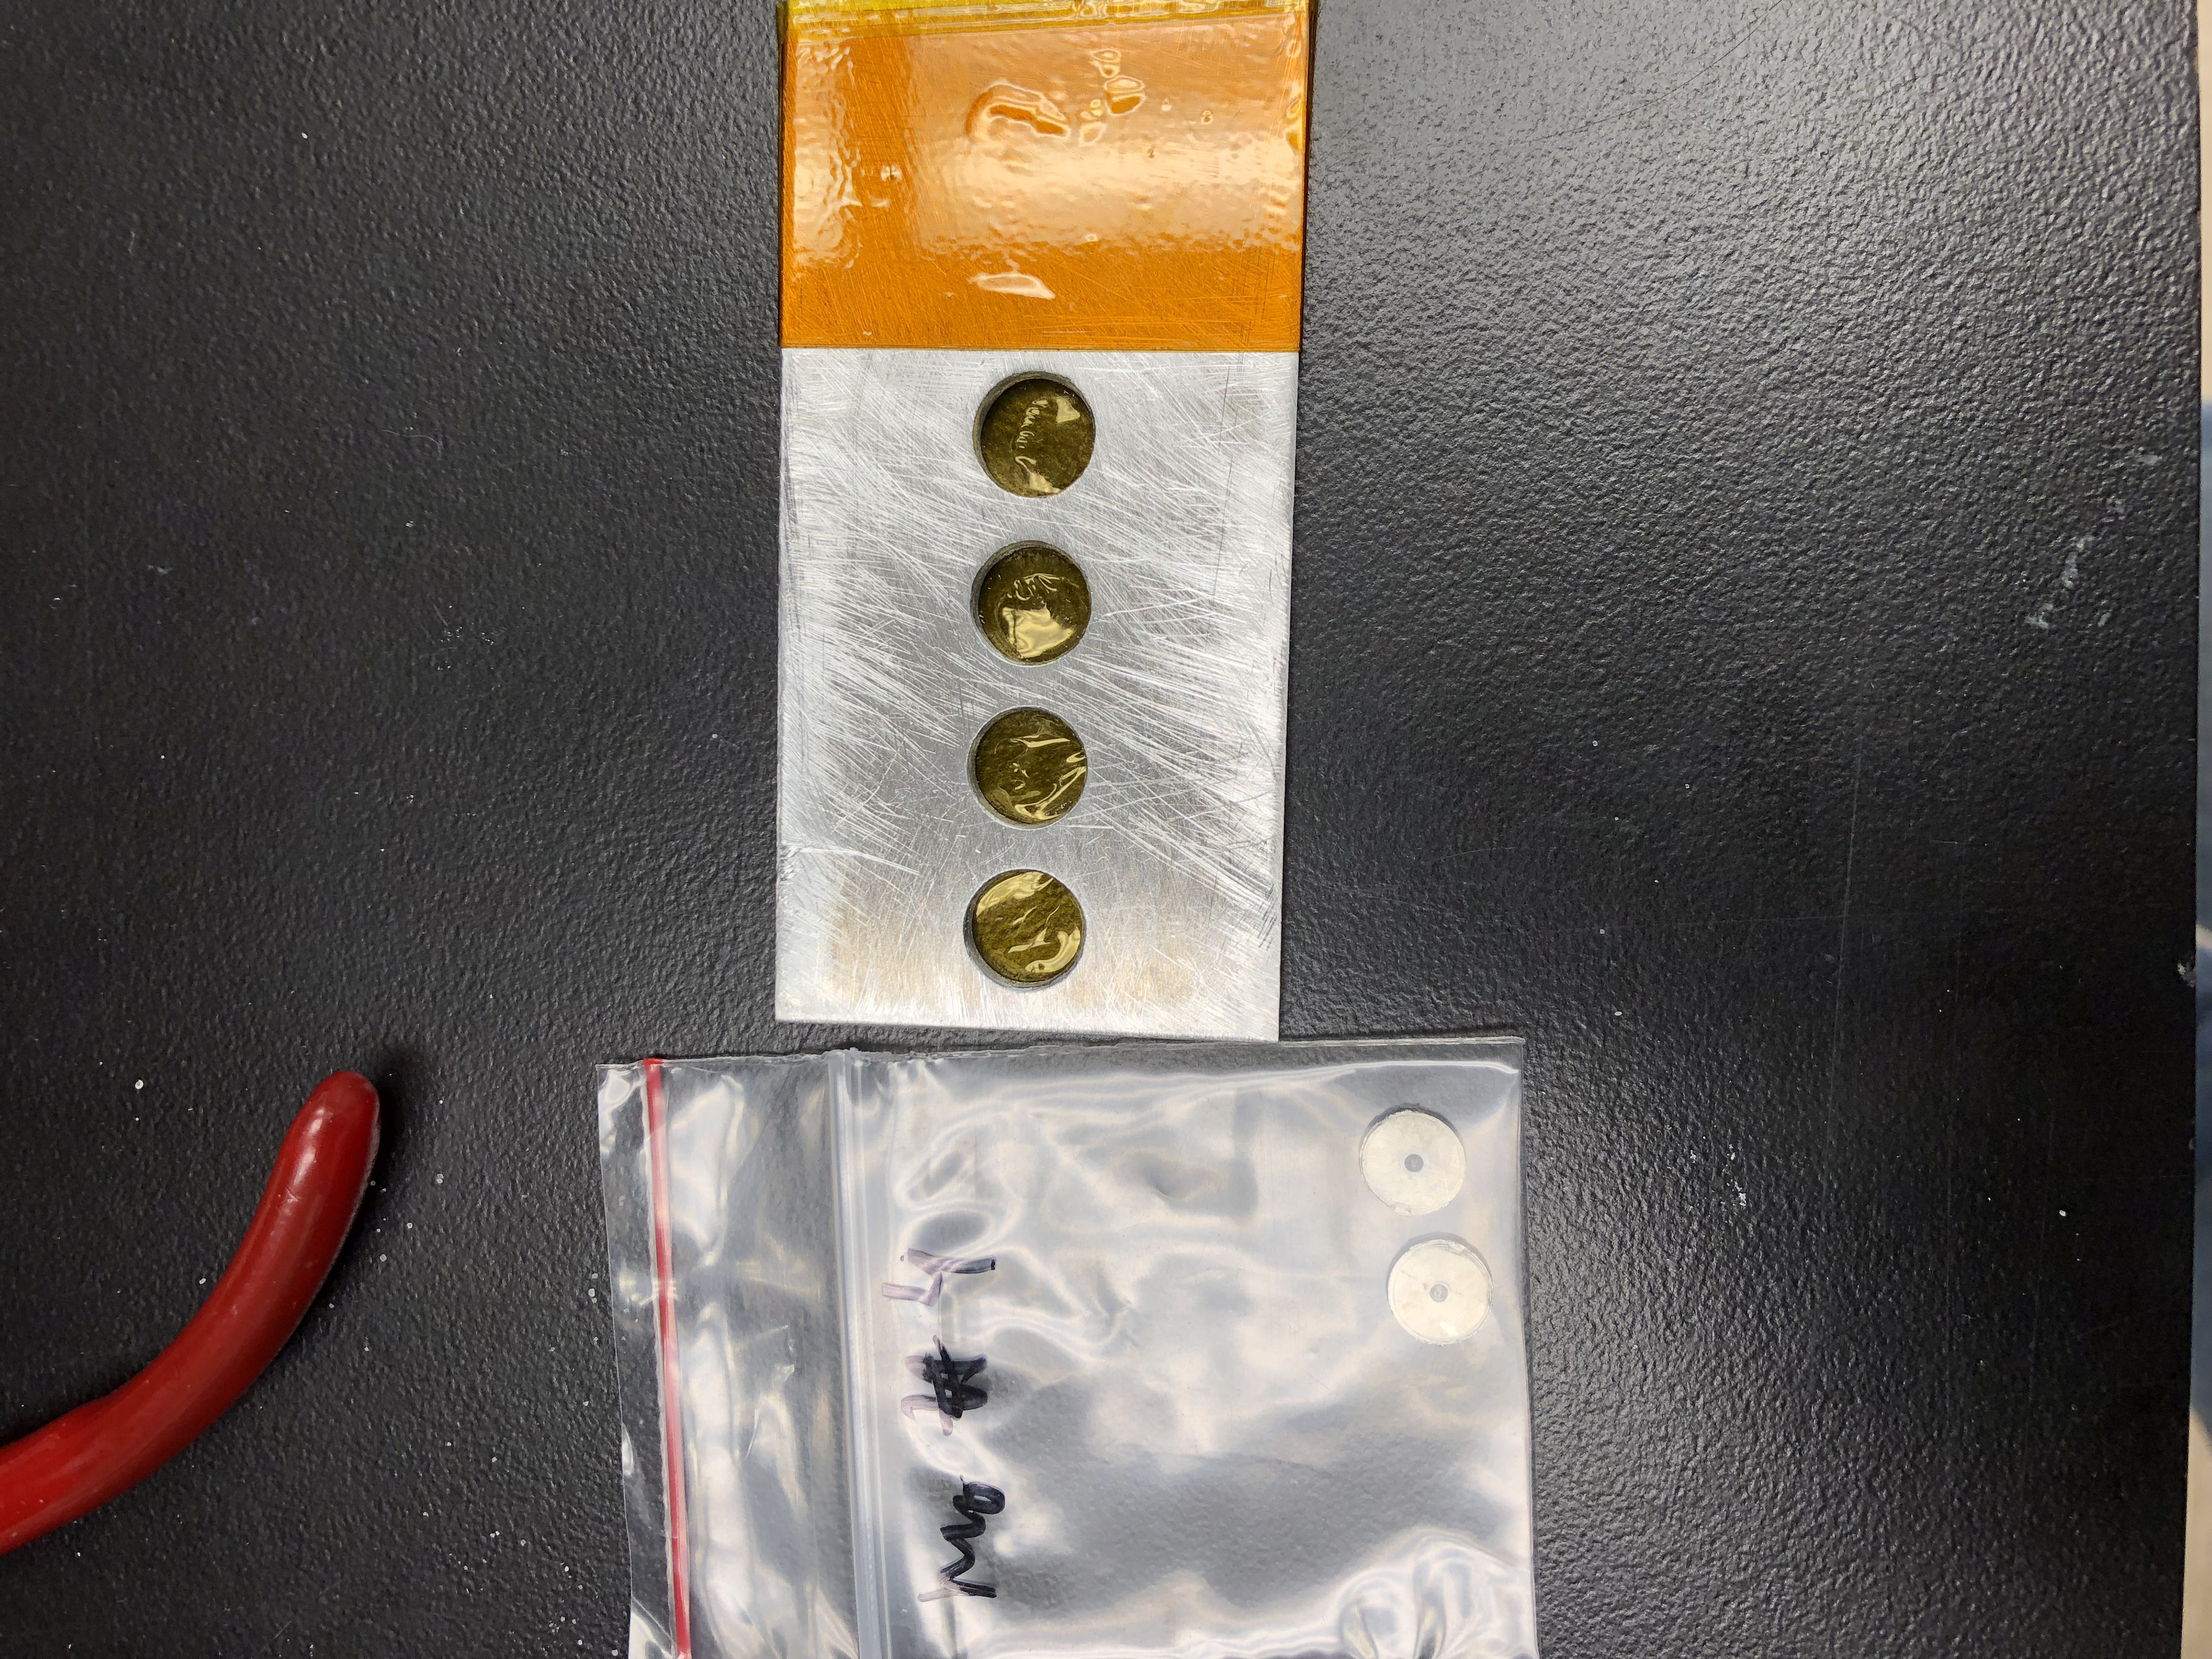
\includegraphics[clip=true,trim=5pt 1000pt 10pt 900pt,width=0.75\columnwidth,angle=90]{./figures/IMG_8840.JPG}
%  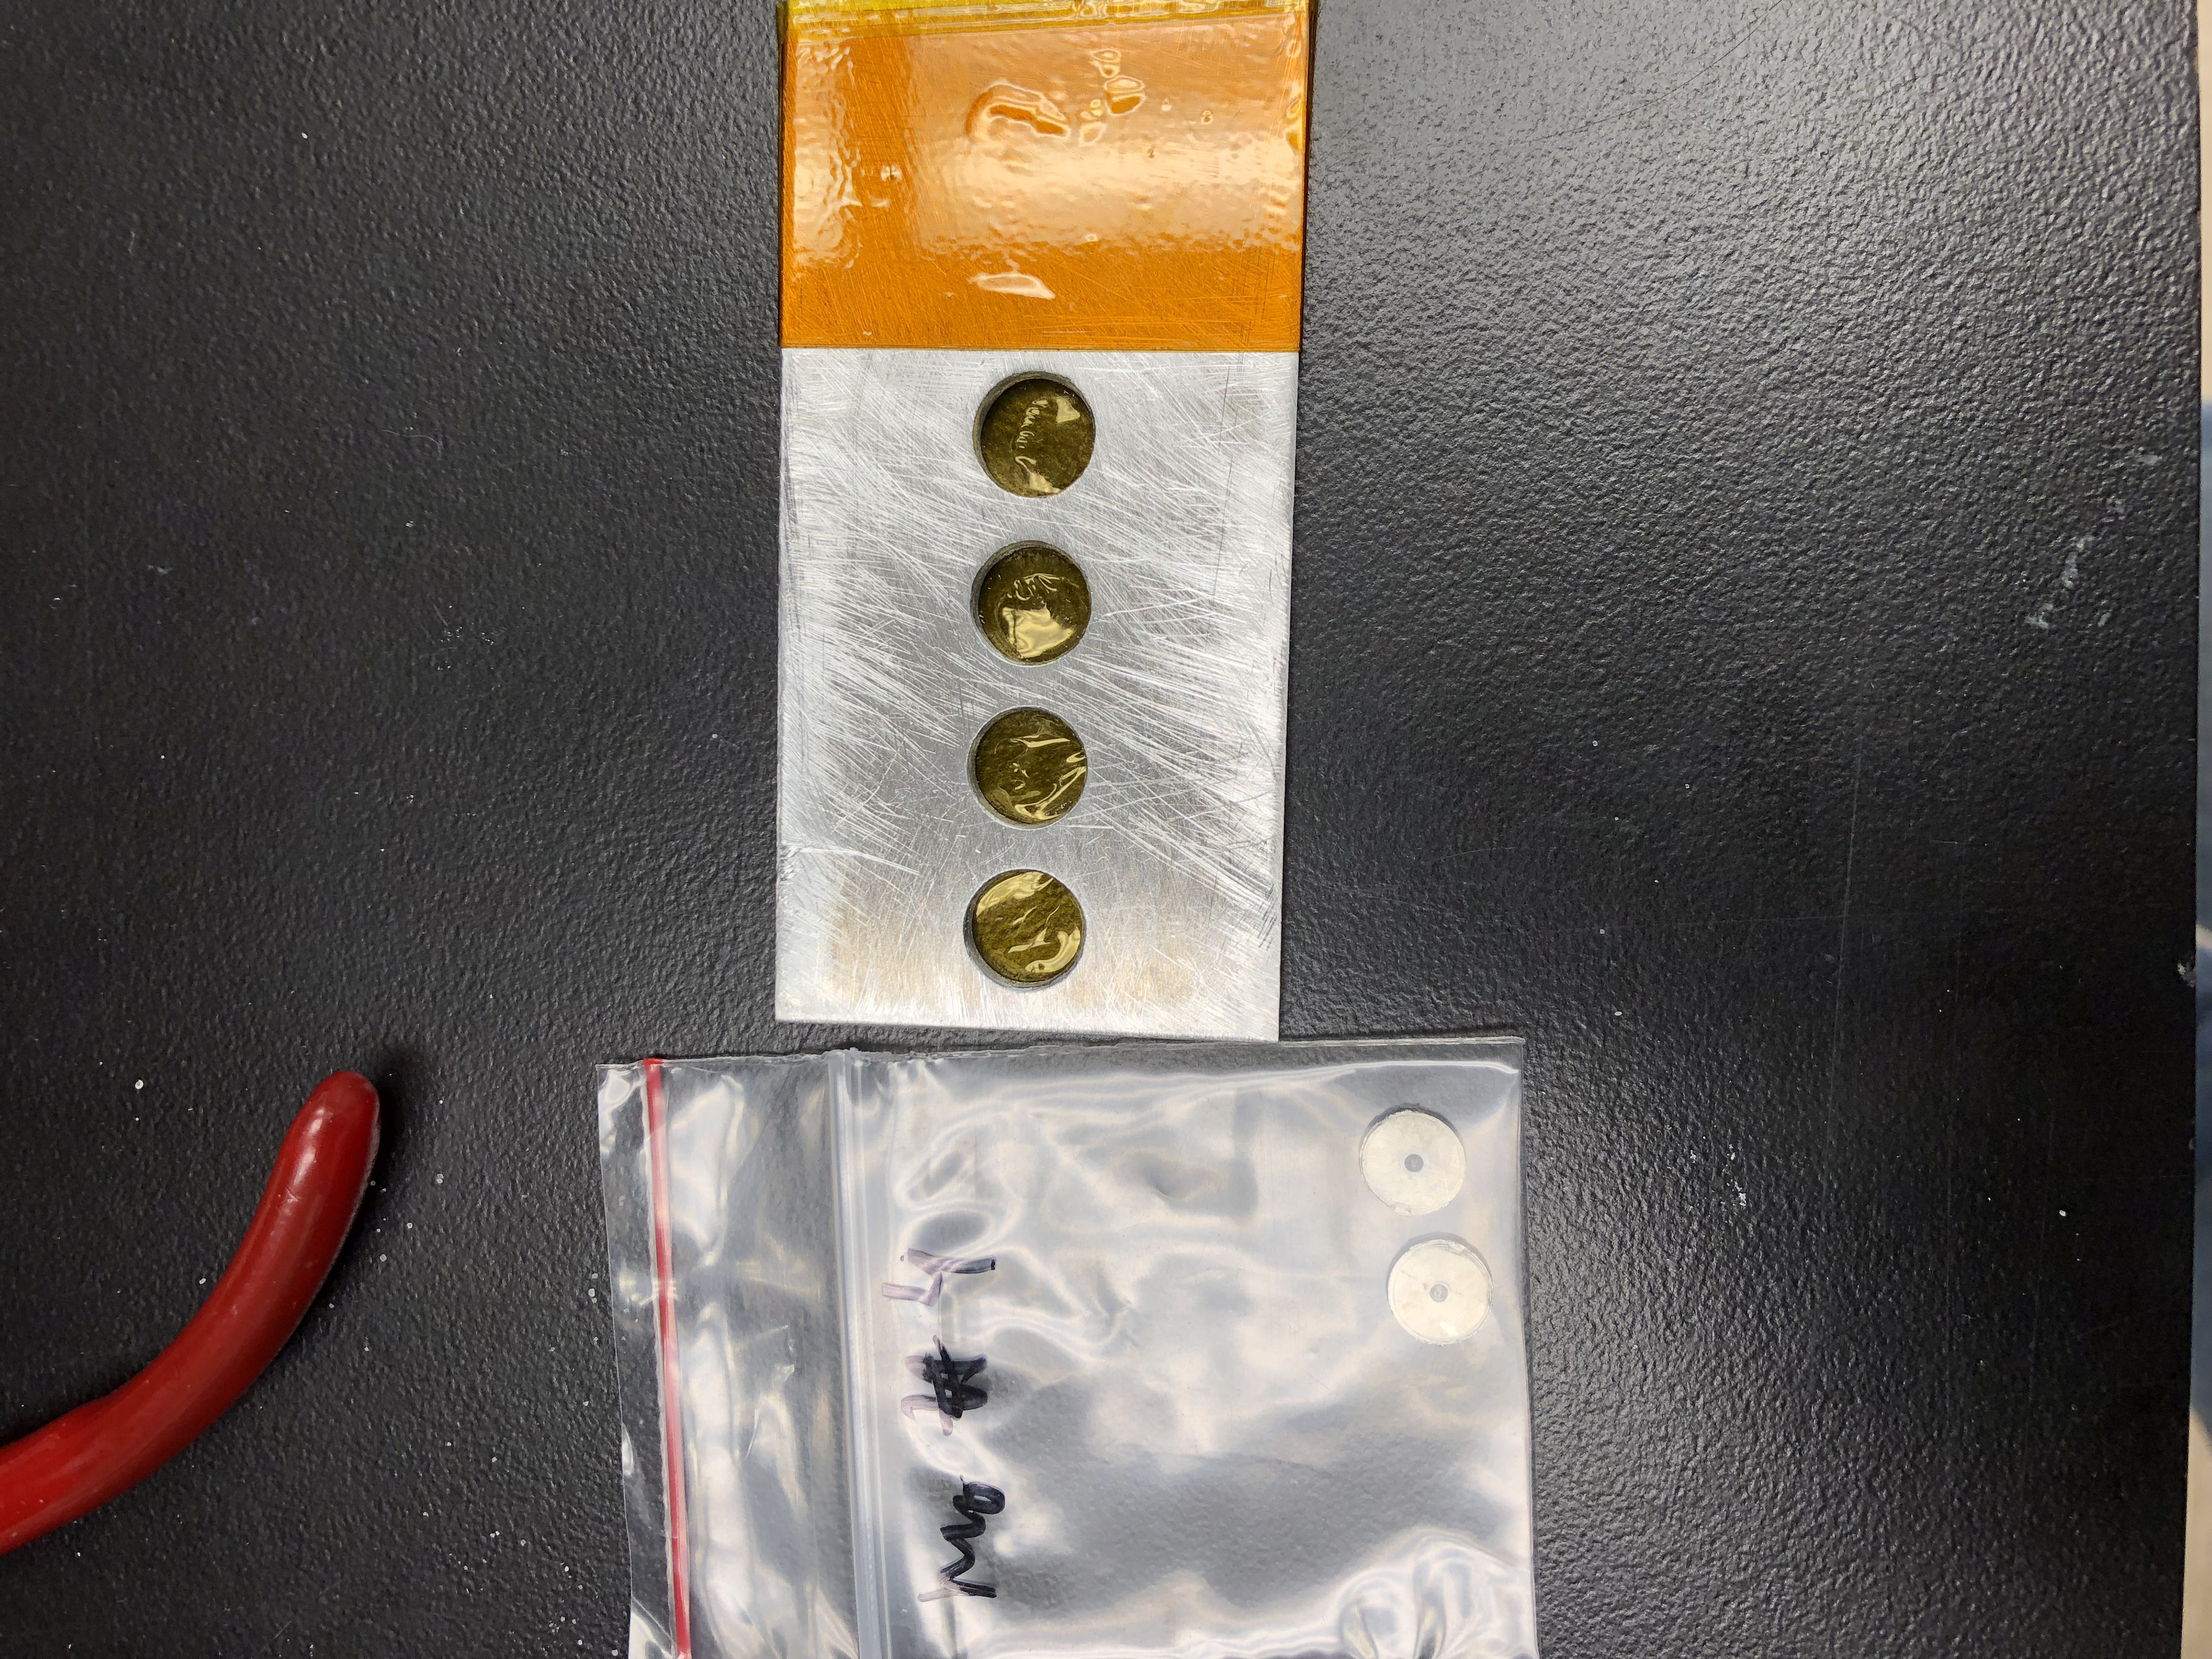
\includegraphics[width=0.75\columnwidth,angle=270]{./figures/IMG_8840.JPG}
 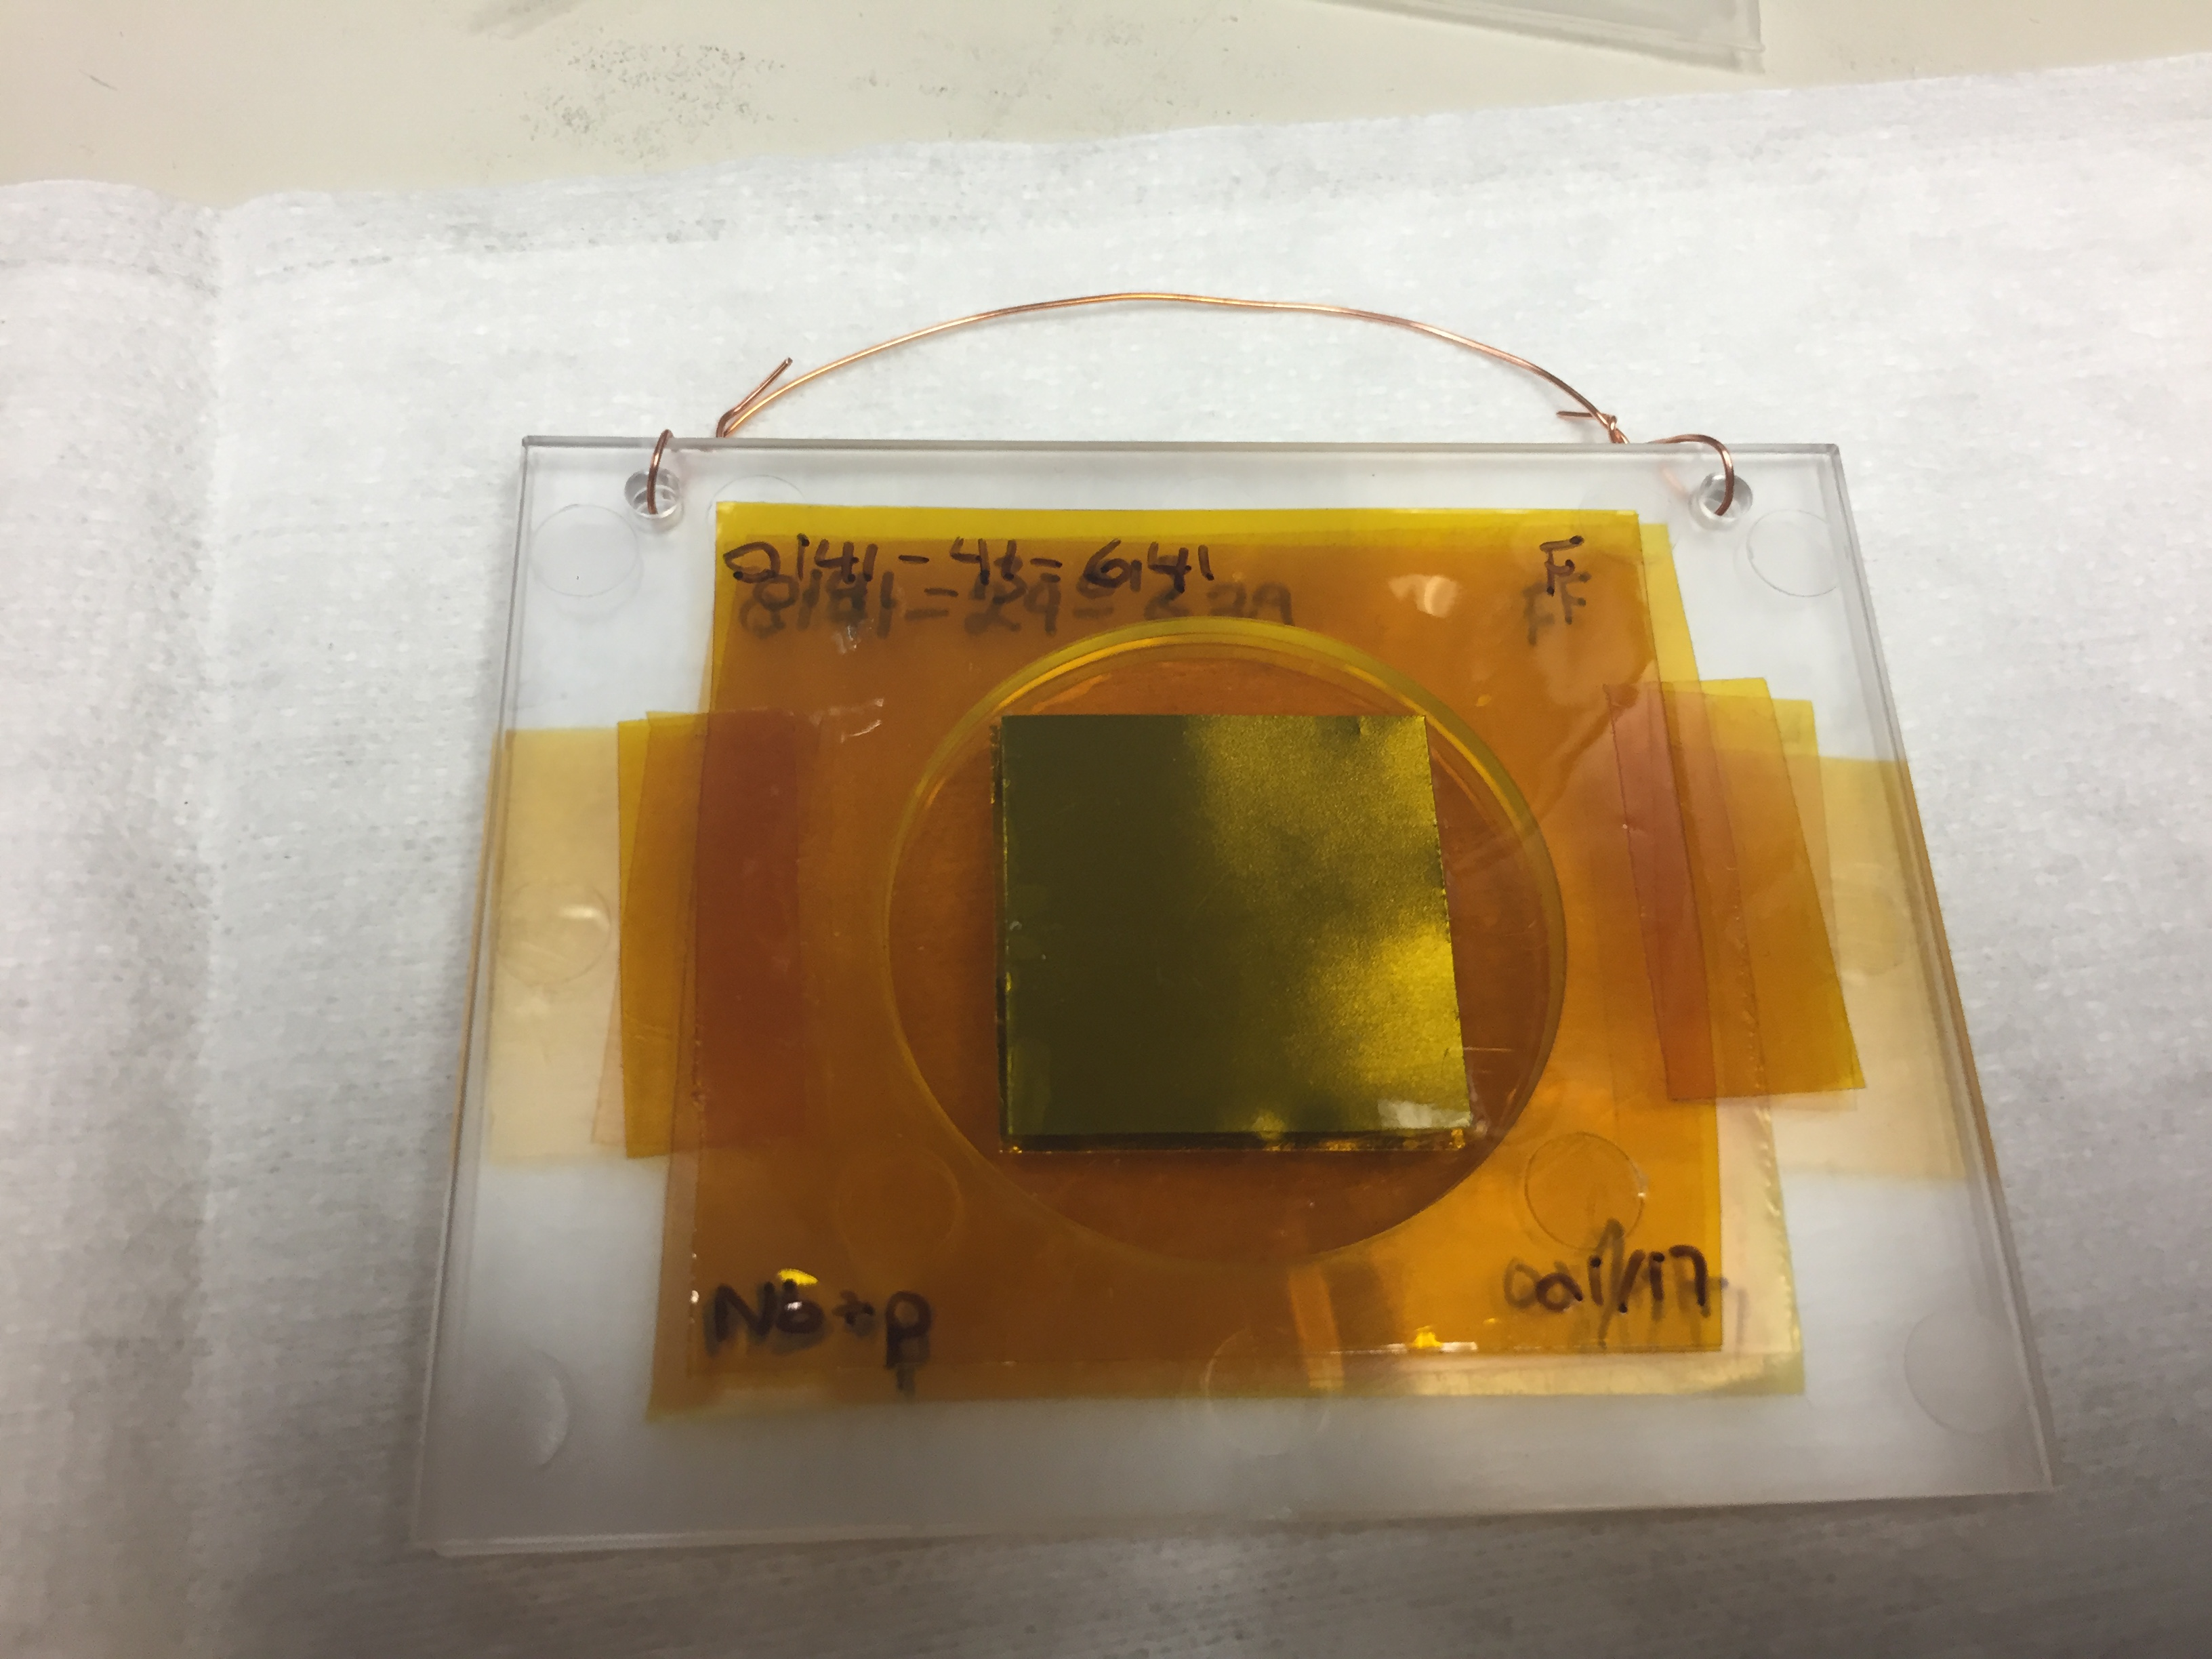
\includegraphics[width=0.75\columnwidth]{./figures/IMG_1969.JPG}
 % IMG_8840.JPG: 4032x3024 pixel, 72dpi, 142.24x106.68 cm, bb=0 0 4032 3024
 \caption{A stacked bundle of Nb (visible on top), Cu, and Al activation foils, for the 60\,MeV position of the Nb(p,x) target stack. All foils are mounted over the aperture of a 1.575 mm-thick plastic frame and bundled together with baling wire.}
 \label{fig:IMG_1969}
\end{figure}



\begin{figure}
 \centering
%                                l   b      r    top
%  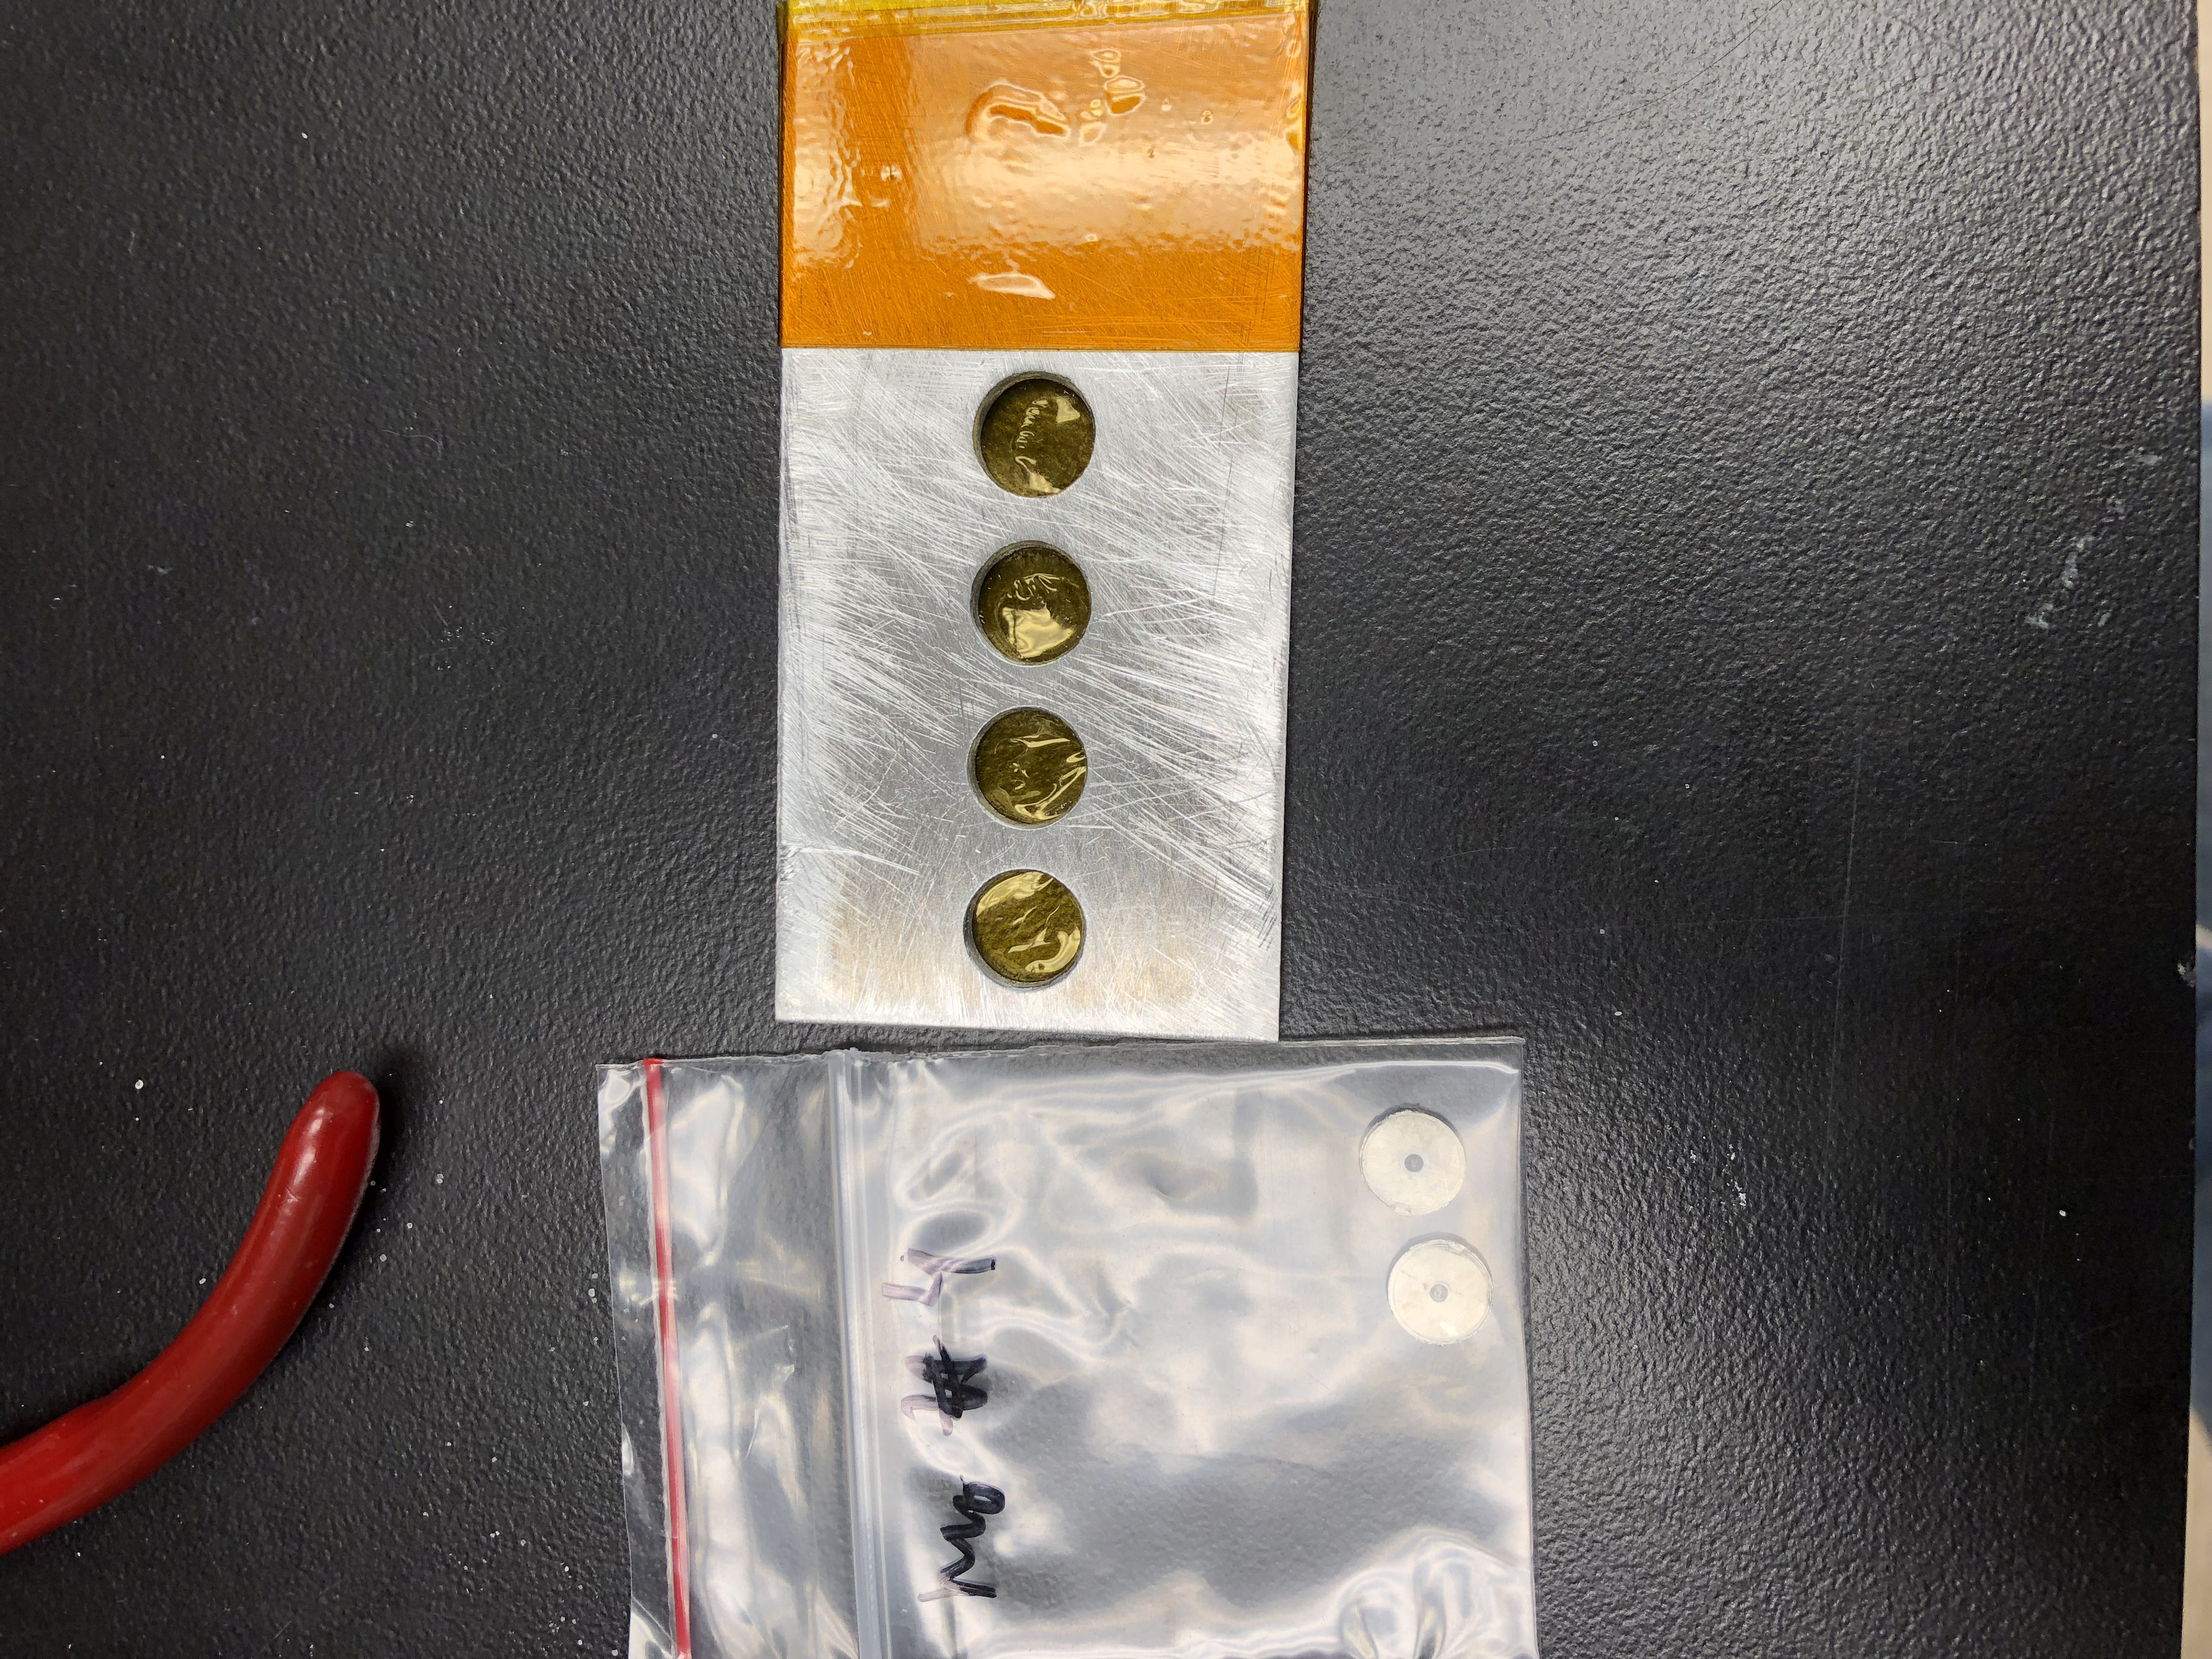
\includegraphics[clip=true,trim=5pt 1000pt 10pt 900pt,width=0.75\columnwidth,angle=90]{./figures/IMG_8840.JPG}
%  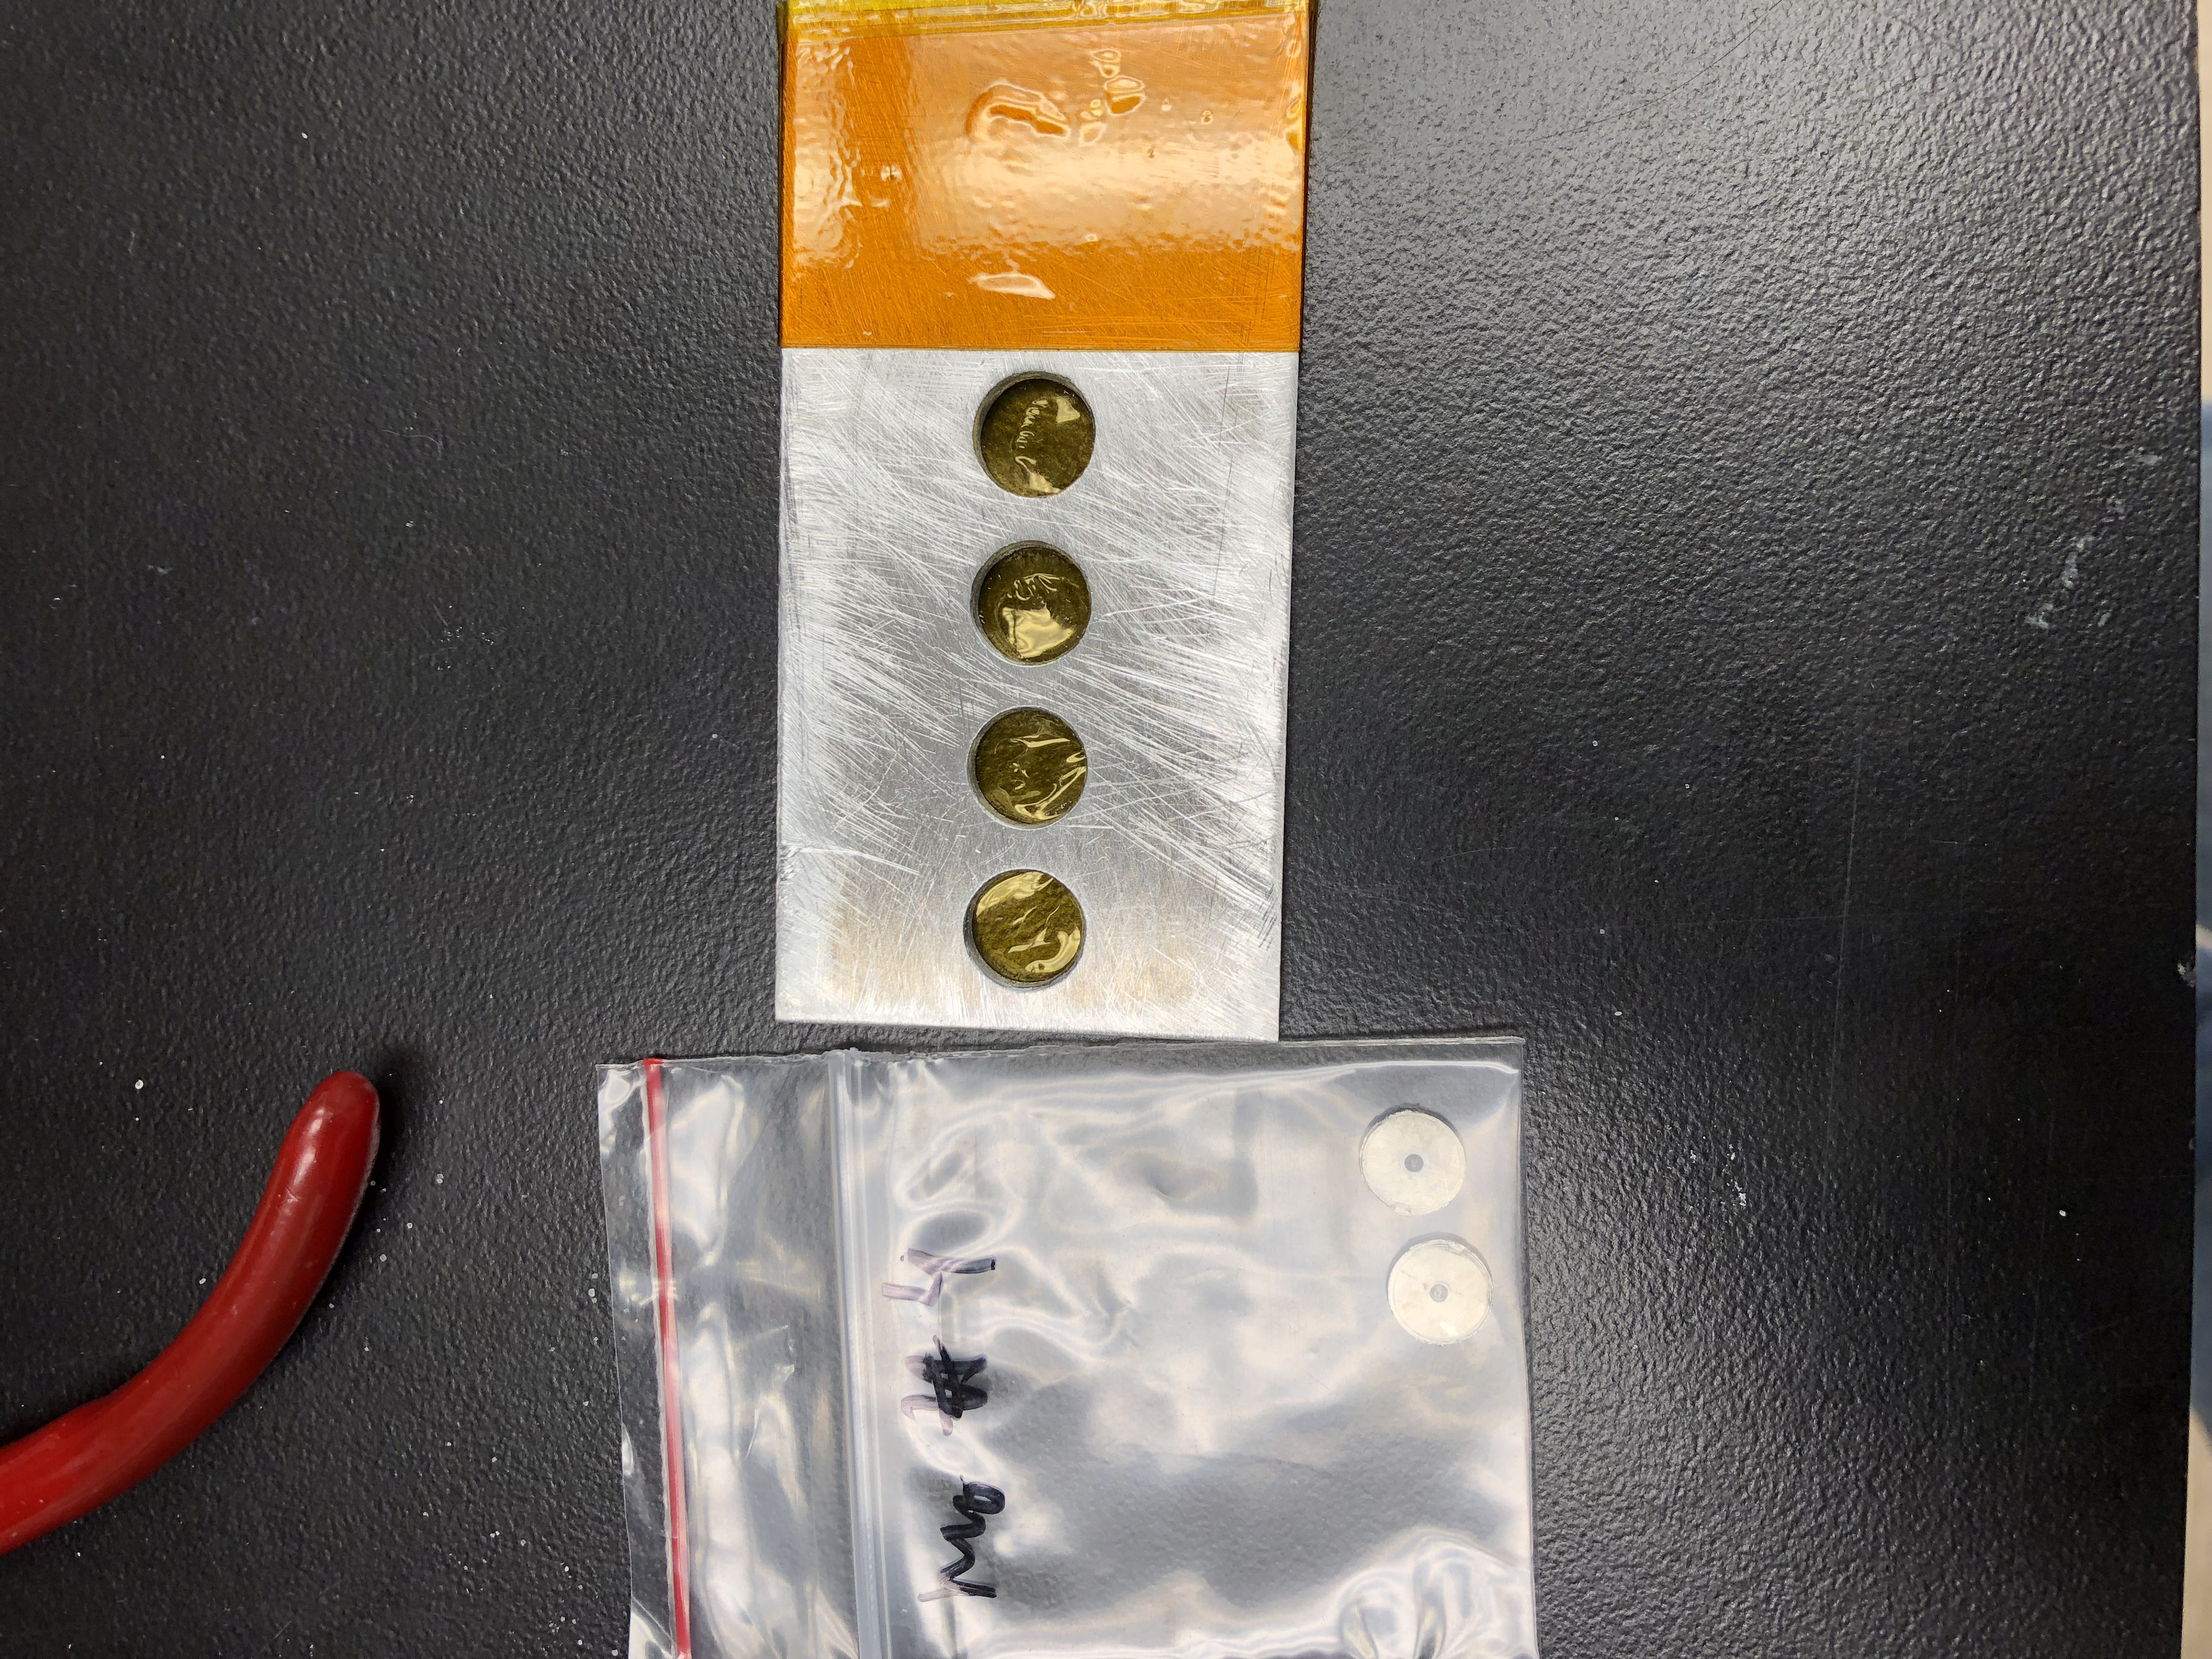
\includegraphics[width=0.75\columnwidth,angle=270]{./figures/IMG_8840.JPG}
 \includegraphics[width=0.75\columnwidth]{./figures/image2993.png}
 % IMG_8840.JPG: 4032x3024 pixel, 72dpi, 142.24x106.68 cm, bb=0 0 4032 3024
 \caption{The IPF hot cell, used for lowering and retrieving the target stack (circled in black) and polyethylene beam profile monitors from the IPF beamline. Robotic manipulators are used for handling of all components in the hot cell, including mounting them onto a motorized track for insertion into the beamline. This track and mount are seen circled in red.}
 \label{fig:IMG_1984}
\end{figure}



\subsubsection{MCNP modeling}




A rendering of the IPF Nb(p,x) target stack, as modeled in MCNP6, is seen in \autoref{fig:ipf_vised}.
% This figure presents a small subset of the full MCNP6 model of the HFNG,  to better illustrate the geometry of the target chamber.
This model is the same described in \autoref{sec:proton_transport} for simulation of proton transport.
The full input file for this MCNP model is included here for reference, in Appendix \ref{sec:ipf_mcnp_deck}.
In this figure, the 100\,MeV proton beam enters from the left of the figure, where it is incident (in the positive $x$ direction) upon the Inconel beam entrance window (yellow).
The other stack elements, described in  \autoref{tab:stack_table} are illustrated here, as well.
The green cell is the cooling water channel for the target box, the air filling the target box is shown in light blue, and the 6061 aluminum beam degraders are shown in dark blue.  
The thin black lines seen in between degraders are the Nb, Cu, and Al activation points at each energy position, sealed in Kapton tape. 
The detail of each foil sealed in the Kapton is not visible here, simply due to the size scale of the stack assembly.


\begin{figure}
 \centering
 %trim option's parameter order: left bottom right top
 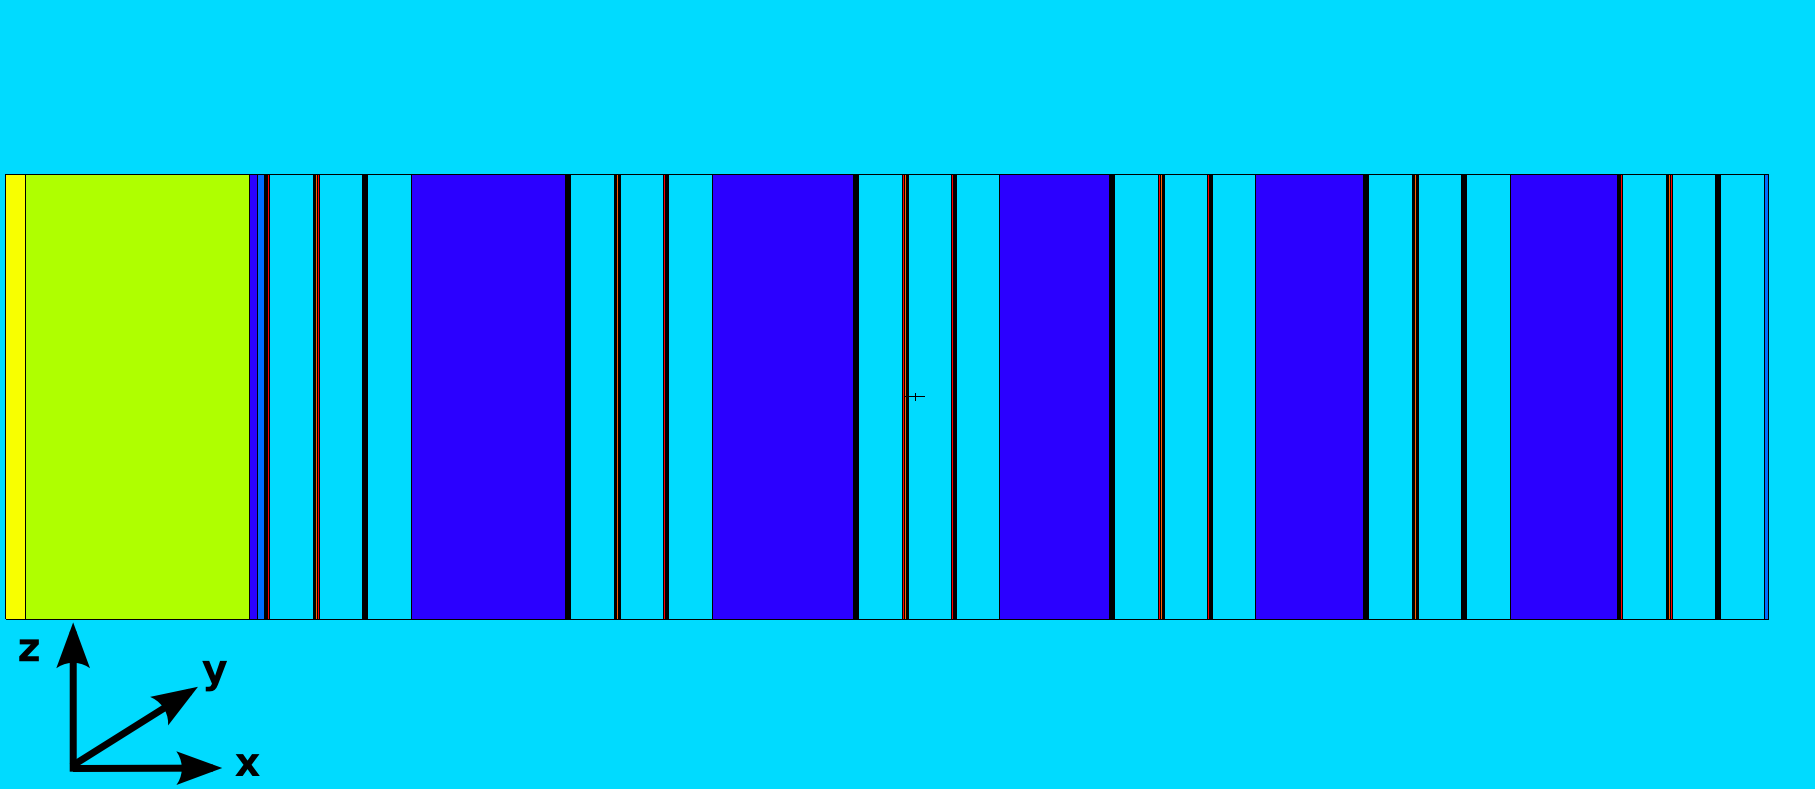
\includegraphics[trim = 0mm 0mm 2mm 0mm, clip,width=0.75\columnwidth]{./figures/ipf_stack_nolabels_axes.PNG}
 % mcnp_vised2.PNG.png: 688x443 pixel, 96dpi, 18.21x11.72 cm, bb=0 0 516 332
 \caption{Simplified top-down MCNP6 model of the IPF Nb(p,x) target stack. The 100\,MeV proton beam enters from the left of the figure, where it is incident upon the Inconel beam entrance window (yellow). The beam is transported down the length of the stack, towards the rear of the stack on the right side of the figure.
%  MCNP6 model of the HFNG target chamber, with reference scale. The co-loaded foils can be seen in the target chamber center.  The ovals indicate the location of water cooling channels.
}
 \label{fig:ipf_vised}
\end{figure}




\begin{figure*}
    \centering    
    \subfloat{
        \centering
%         \includegraphics[width=\textwidth]{./figures/target2.png}
        \subfigimg[width=0.495\textwidth]{a)}{./figures/Al_ptallies.pdf}{80}
%         \caption{Decay curve for the $\beta^-$ decay of \ce{^{116}In}.}
        %         \refstepcounter{subfigure}
%          \label{fig:91mNb}
%    }
%      \subfloat{
%         \centering
%         \includegraphics[width=\columnwidth]{./figures/Capture.PNG}
        \subfigimg[width=0.495\textwidth]{b)}{./figures/Cu_ptallies.pdf}{80}
%         \caption{ Decay curve for the $\beta^+$ decay of \ce{^{64}Cu}.}
%         \refstepcounter{subfigure} 
%         \label{fig:92mNb}
   \hspace{-10pt}}%
    \caption{Final variance minimized incident proton energy distributions for the (a) Al and (b) Cu foils, as simulated in MCNP6. The distribution tallies in each foil are all normalized to be per source proton, which was $10^8$ in all simulations. As the beam is degraded, proton energy distributions become visibly broadened due to straggling, and drop in magnitude due to scattering losses.}
%      \phantomcaption{}
     \label{fig:ipf_ptallies_appendix}
\end{figure*}



Using this MCNP6 model, the proton energy distribution is tallied in all volumes of the stack assembly.
As seen in \autoref{fig:Nb_ptallies} of \autoref{sec:proton_transport}, the corresponding incident proton  energy distributions $\frac{d\phi}{dE}$ from MCNP6 simulation (using the variance minimized degrader density) are shown for the six irradiated Cu and Al  foils in \autoref{fig:ipf_ptallies_appendix}. 
In addition, the MCNP6 model tracks the production and transport of secondary neutrons produced through (p,xn) reactions on the target stack components.
The the proton energy distribution is tallied in all Al, Cu, and Nb foils, and is seen in \autoref{fig:ipf_ntallies}. 
The neutron flux is consistently 3--4 orders of magnitude smaller than the corresponding proton flux, and is seen to be visibly  downscattered when moving down the stack.

\begin{figure*}
    \centering    
    \subfloat{
        \centering
%         \includegraphics[width=\textwidth]{./figures/target2.png}
        \subfigimg[width=0.497\textwidth]{a)}{./figures/Al_ntallies.pdf}{50}
%         \caption{Decay curve for the $\beta^-$ decay of \ce{^{116}In}.}
        %         \refstepcounter{subfigure}
%          \label{fig:91mNb}
%    }
%      \subfloat{
%         \centering
%         \includegraphics[width=\columnwidth]{./figures/Capture.PNG}
        \subfigimg[width=0.497\textwidth]{b)}{./figures/Cu_ntallies.pdf}{50}
%         \caption{ Decay curve for the $\beta^+$ decay of \ce{^{64}Cu}.}
%         \refstepcounter{subfigure} 
%         \label{fig:92mNb}
   \hspace{-10pt}}%
    \\
    \subfloat{
        \centering
%         \includegraphics[width=\columnwidth]{./figures/Capture.PNG}
        \subfigimg[width=0.497\textwidth]{c)}{./figures/Nb_ntallies.pdf}{50}
%         \caption{ Decay curve for the isomeric transition of \ce{^{115m}In}.}
%         \refstepcounter{subfigure}
%          \label{fig:93mMo}
   }%
    \caption{Final variance minimized incident neutron energy distributions for the (a) Al, (b) Cu, and (C) Nb foils, as simulated in MCNP6. The distribution tallies in each foil are all normalized to be per source proton, which was $10^8$ in all simulations. As the beam is degraded, neutron energy distributions become visibly downscattered.}
%      \phantomcaption{}
     \label{fig:ipf_ntallies}
\end{figure*}





% \begin{figure}
%  \centering
% %                                l   b      r    top
% %  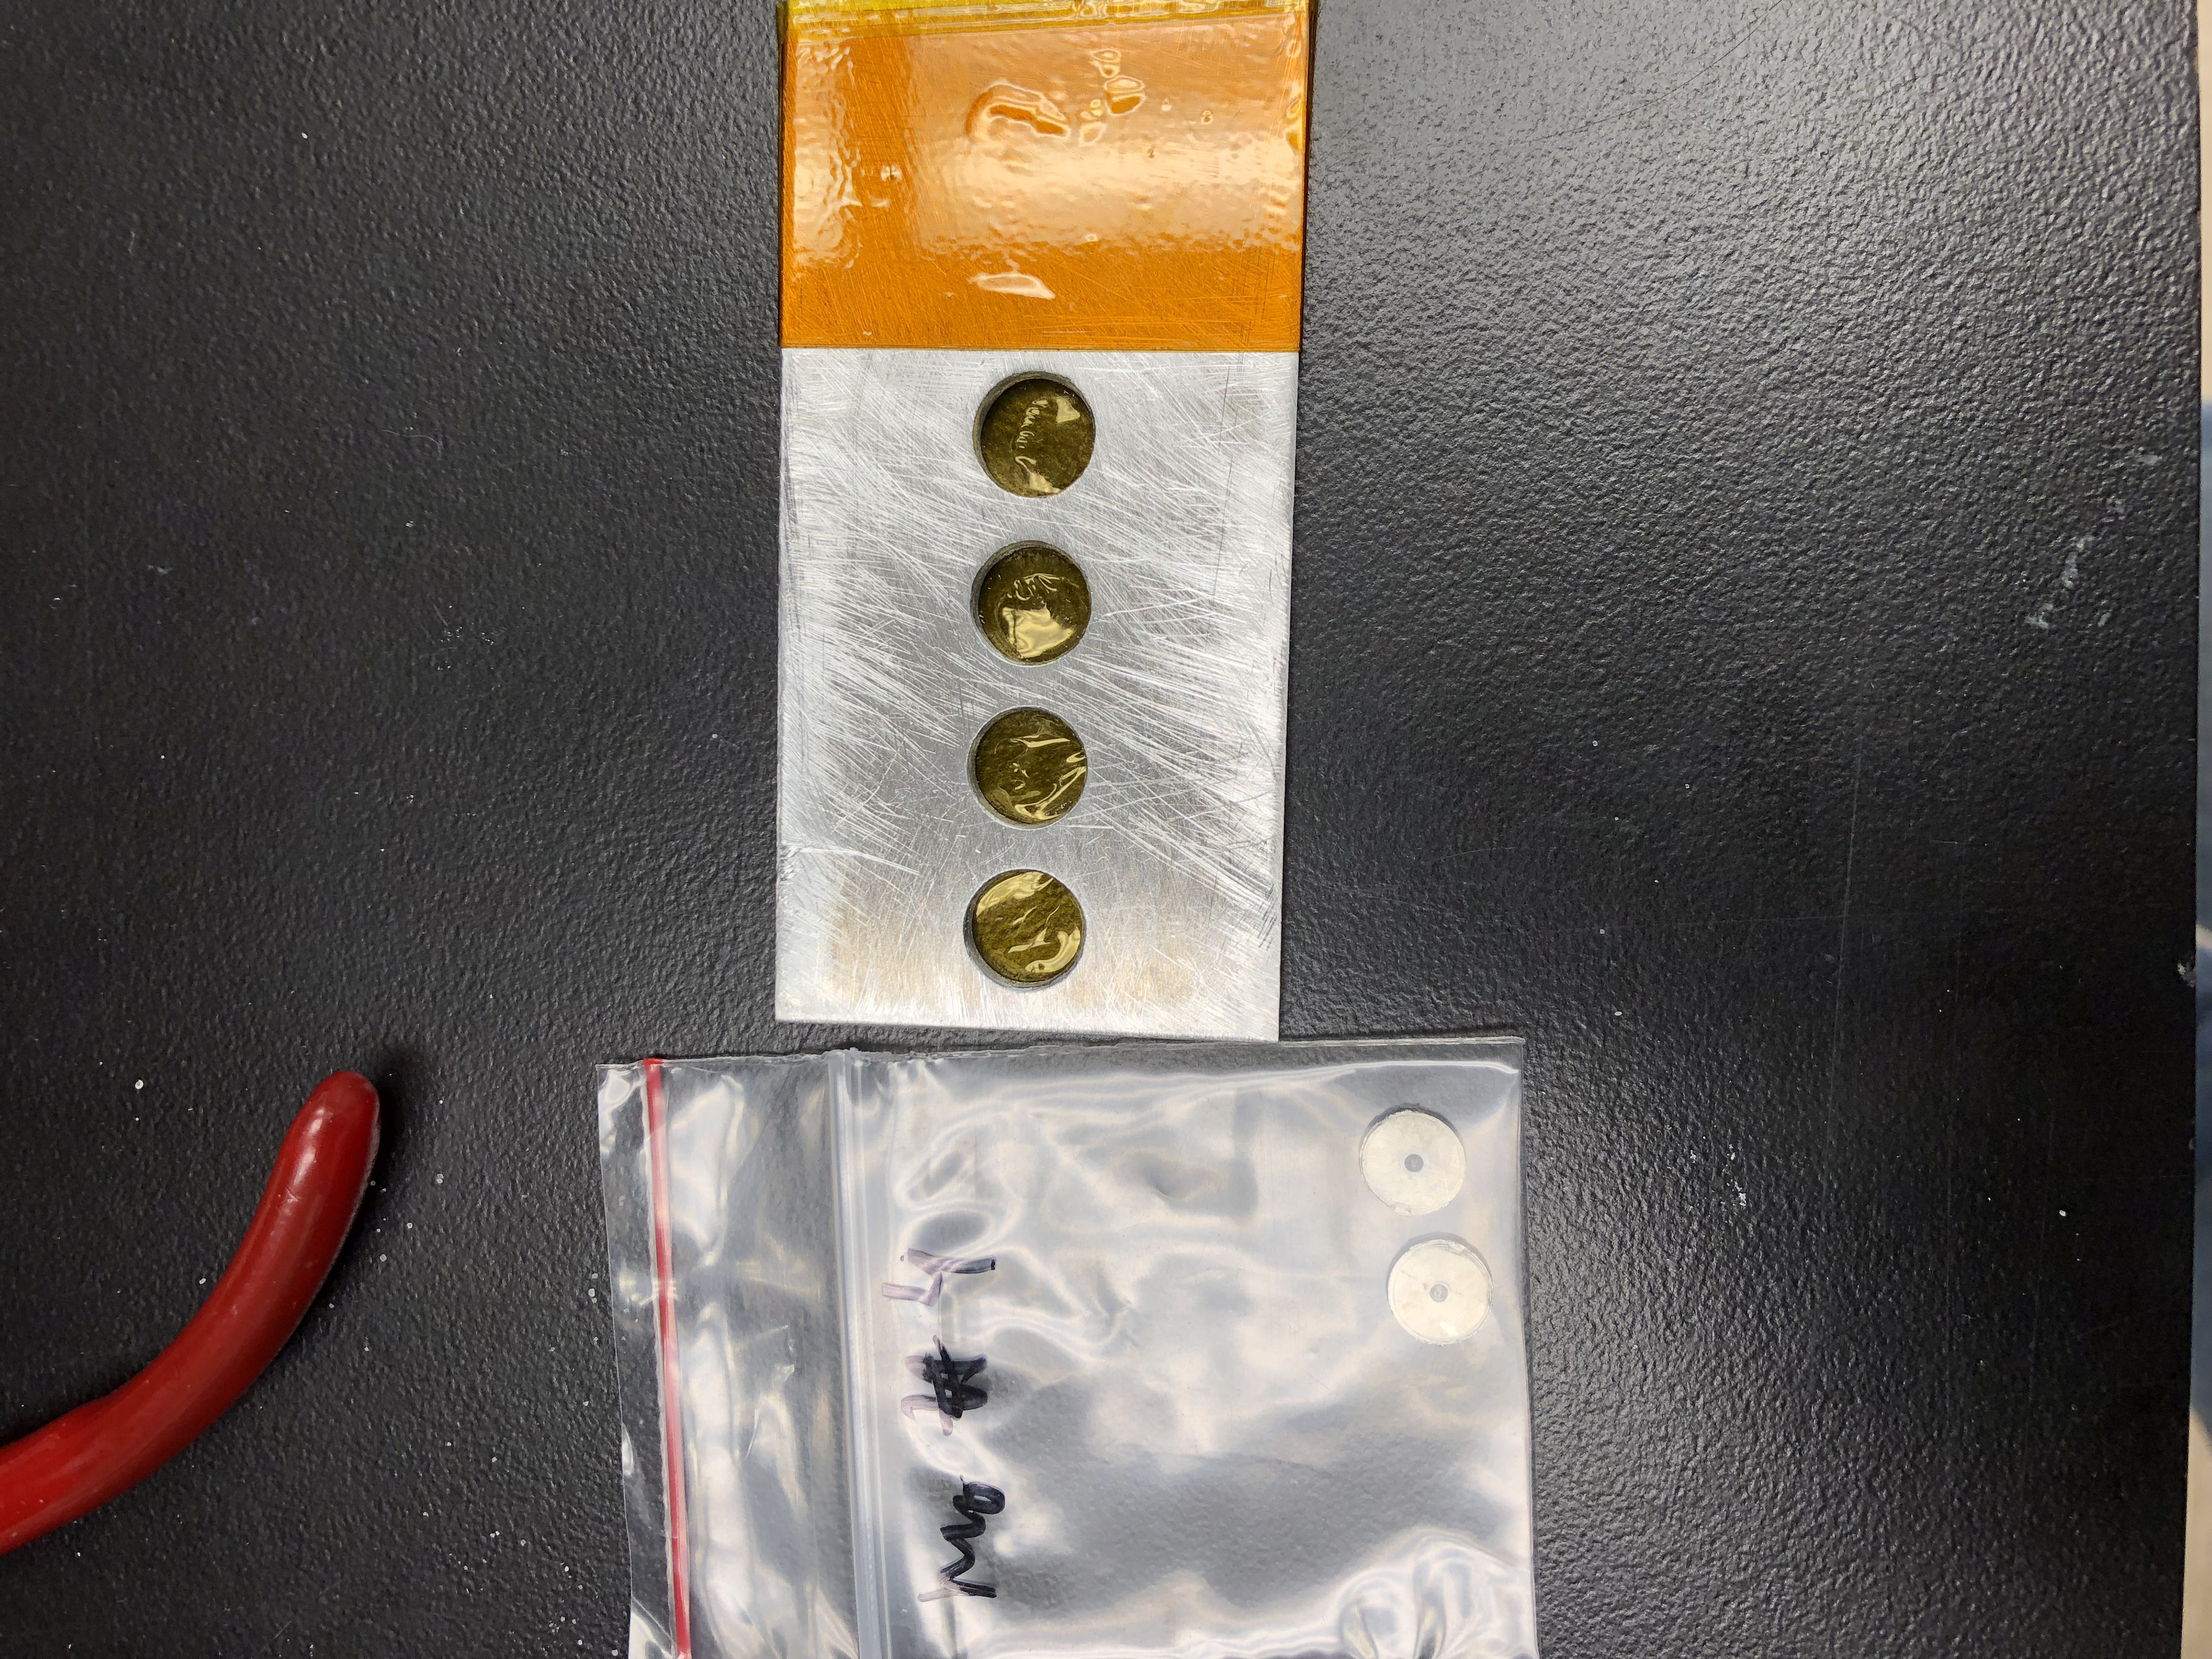
\includegraphics[clip=true,trim=5pt 1000pt 10pt 900pt,width=0.75\columnwidth,angle=90]{./figures/IMG_8840.JPG}
% %  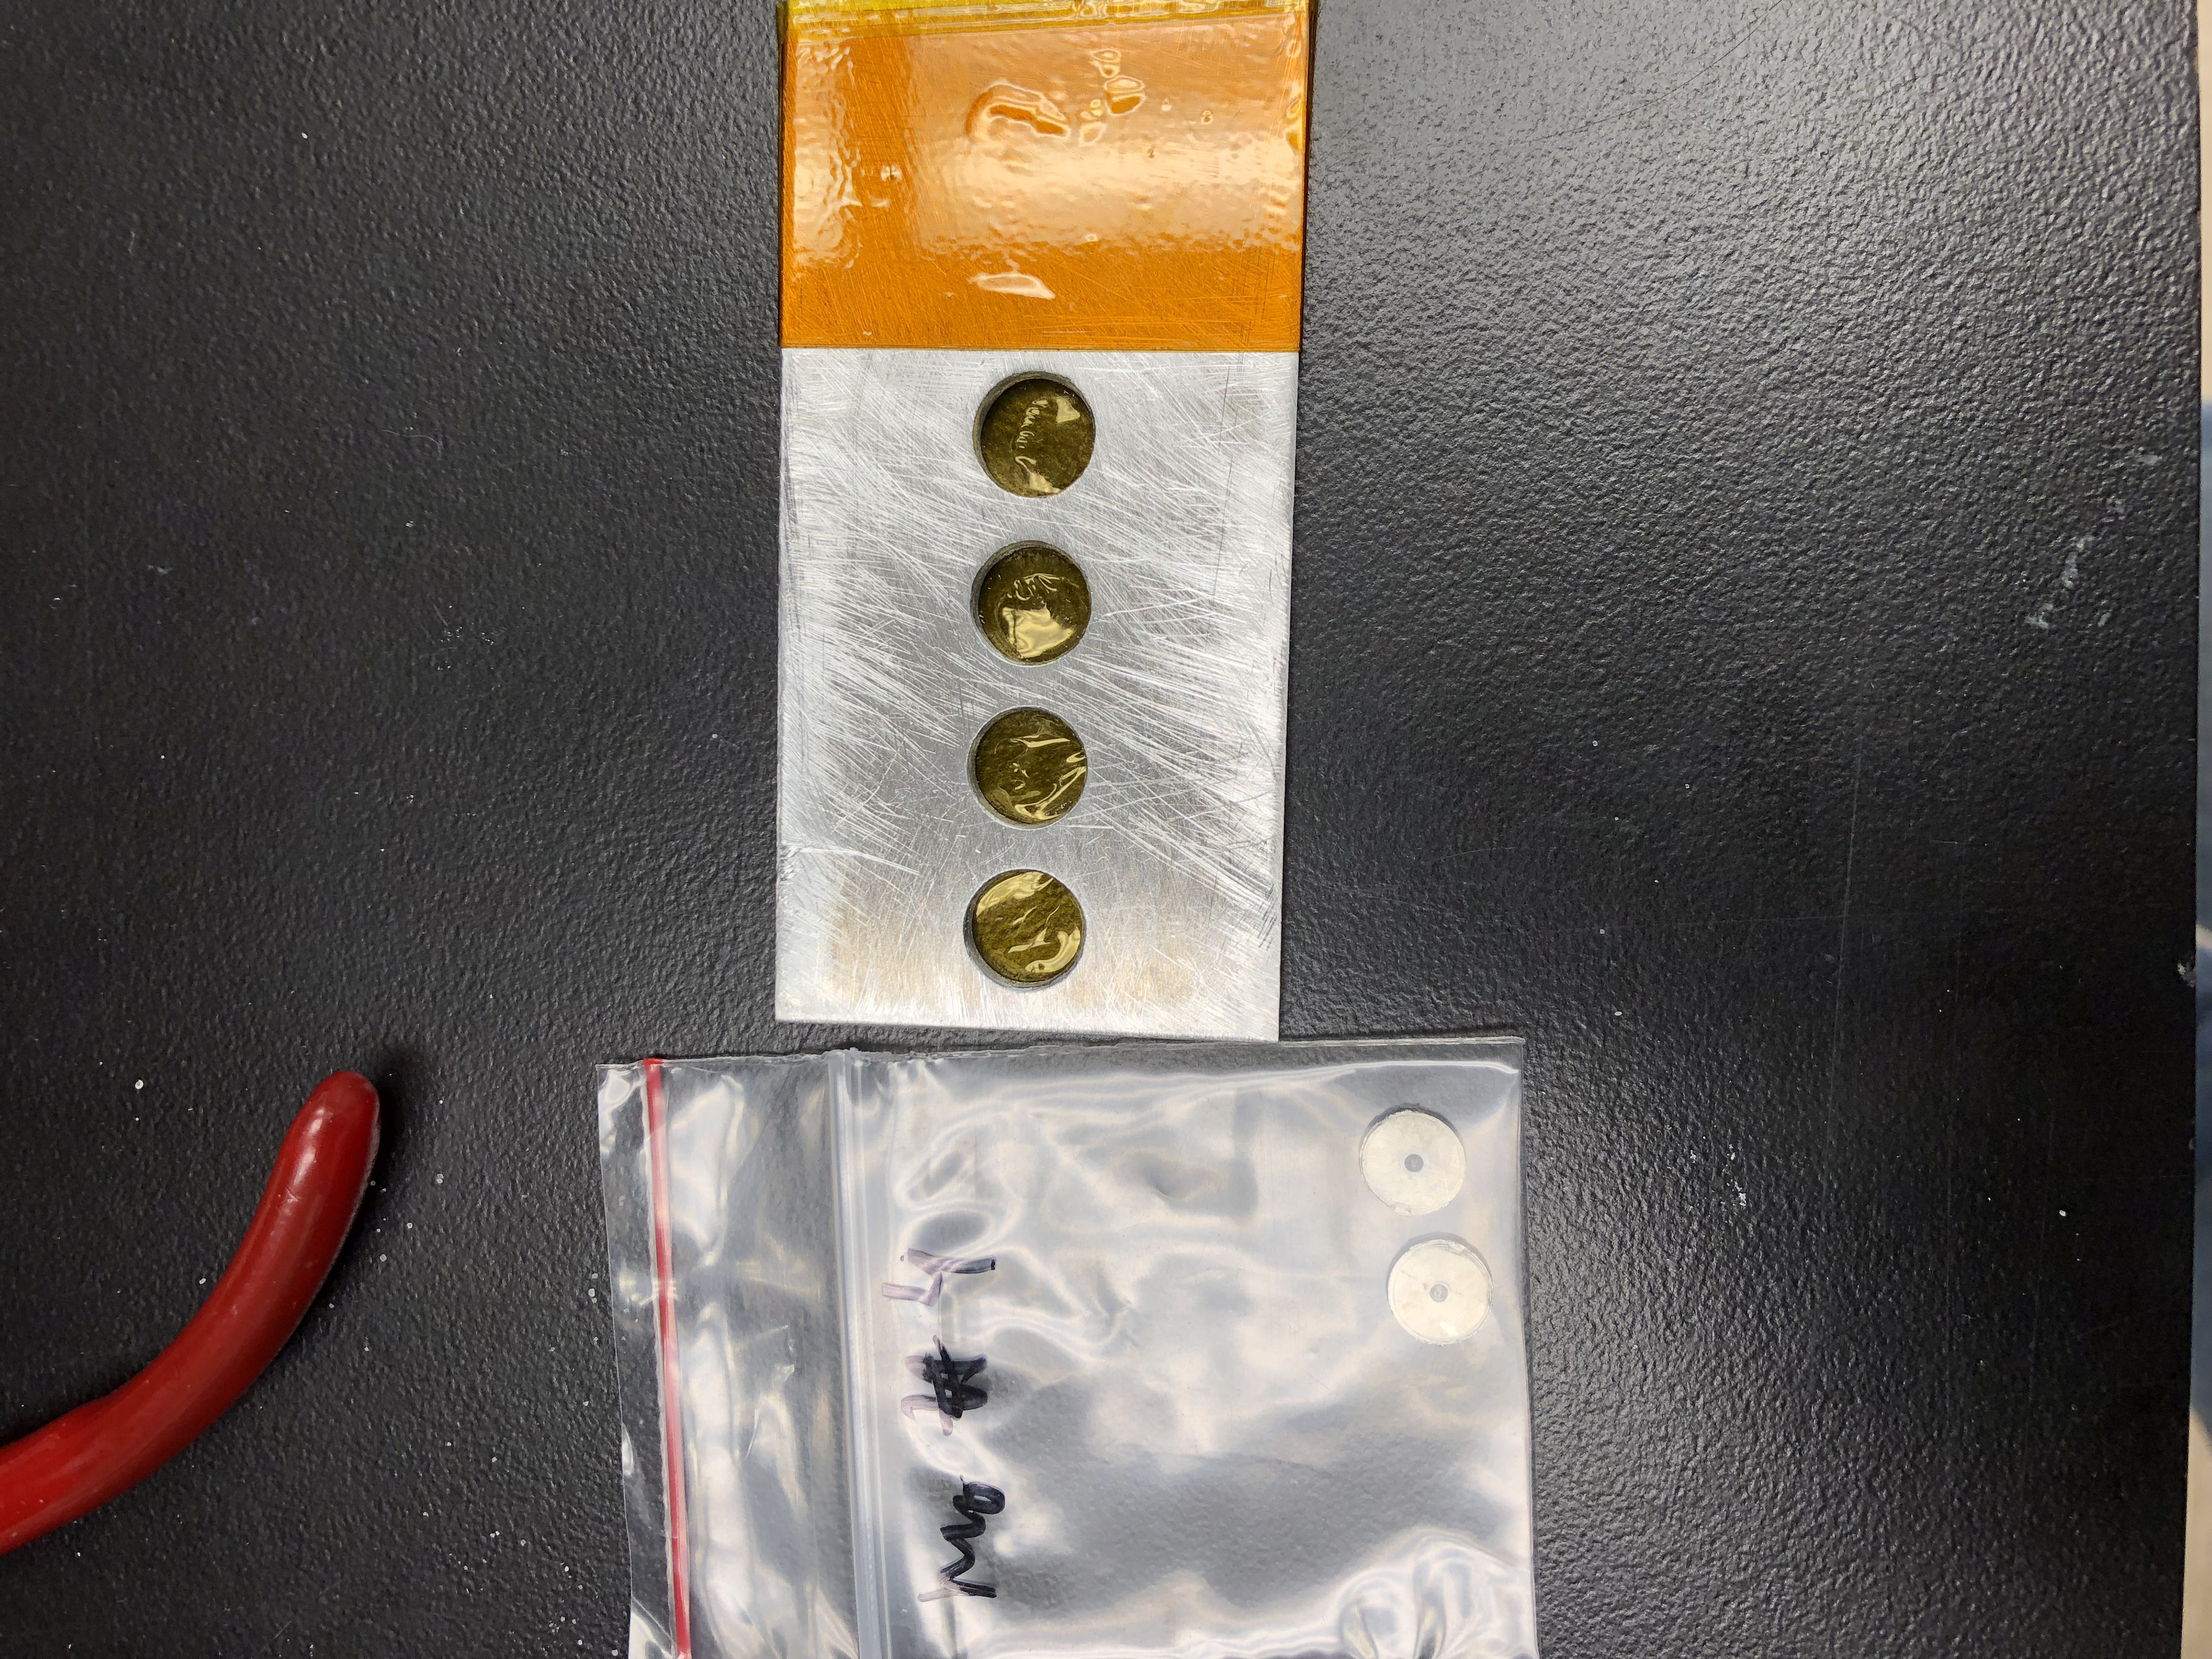
\includegraphics[width=0.75\columnwidth,angle=270]{./figures/IMG_8840.JPG}
%  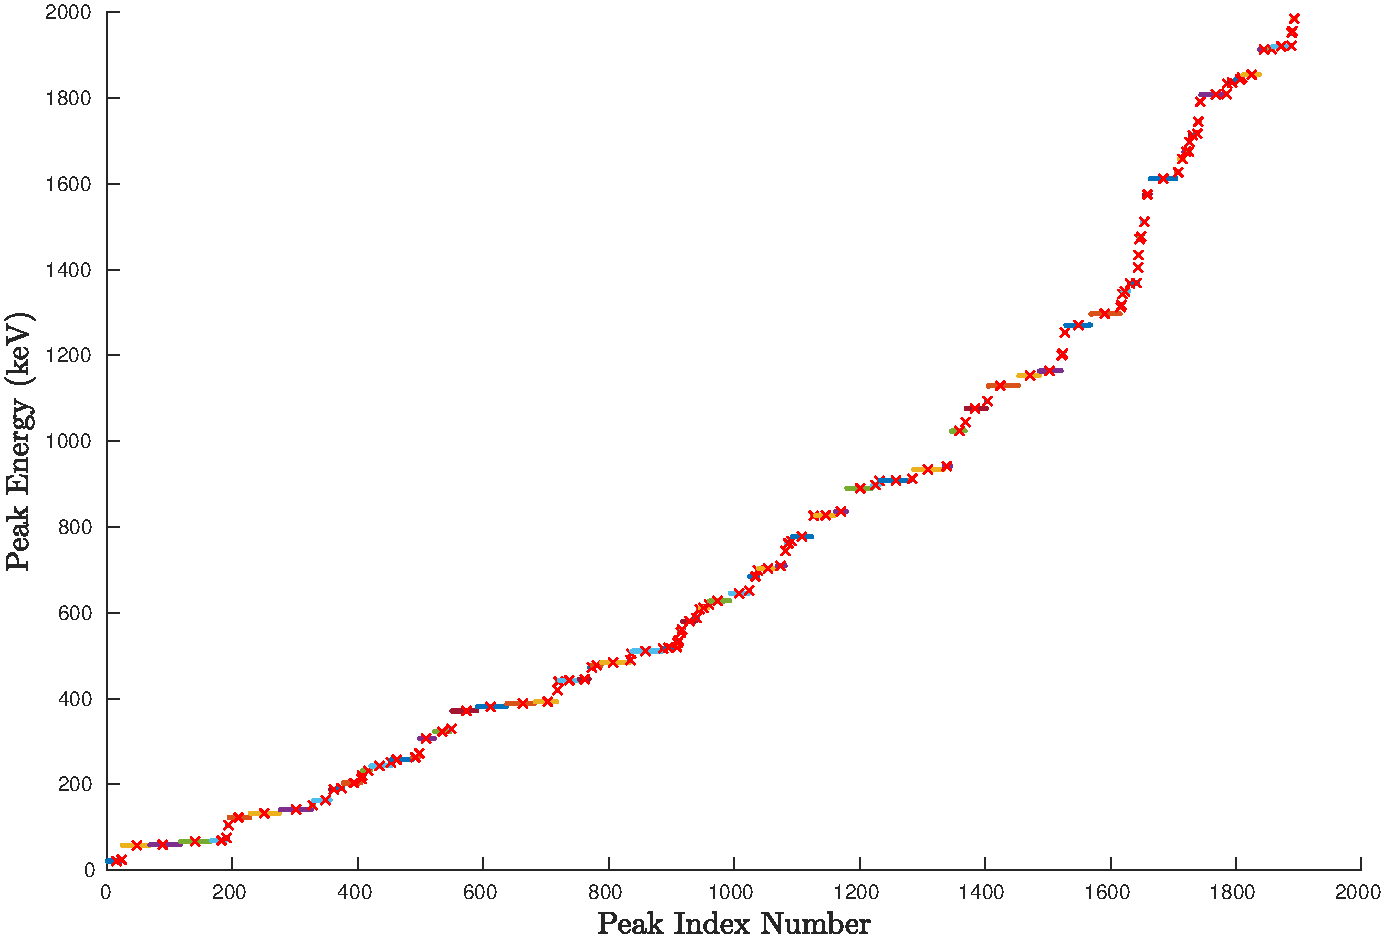
\includegraphics[width=0.75\columnwidth]{./figures/peak_stairsteps.pdf}
%  % IMG_8840.JPG: 4032x3024 pixel, 72dpi, 142.24x106.68 cm, bb=0 0 4032 3024
%  \caption{peak stairsteps.}
%  \label{fig:peak_stairsteps}
% \end{figure}






\begin{figure}
 \centering
%                                l   b      r    top
%  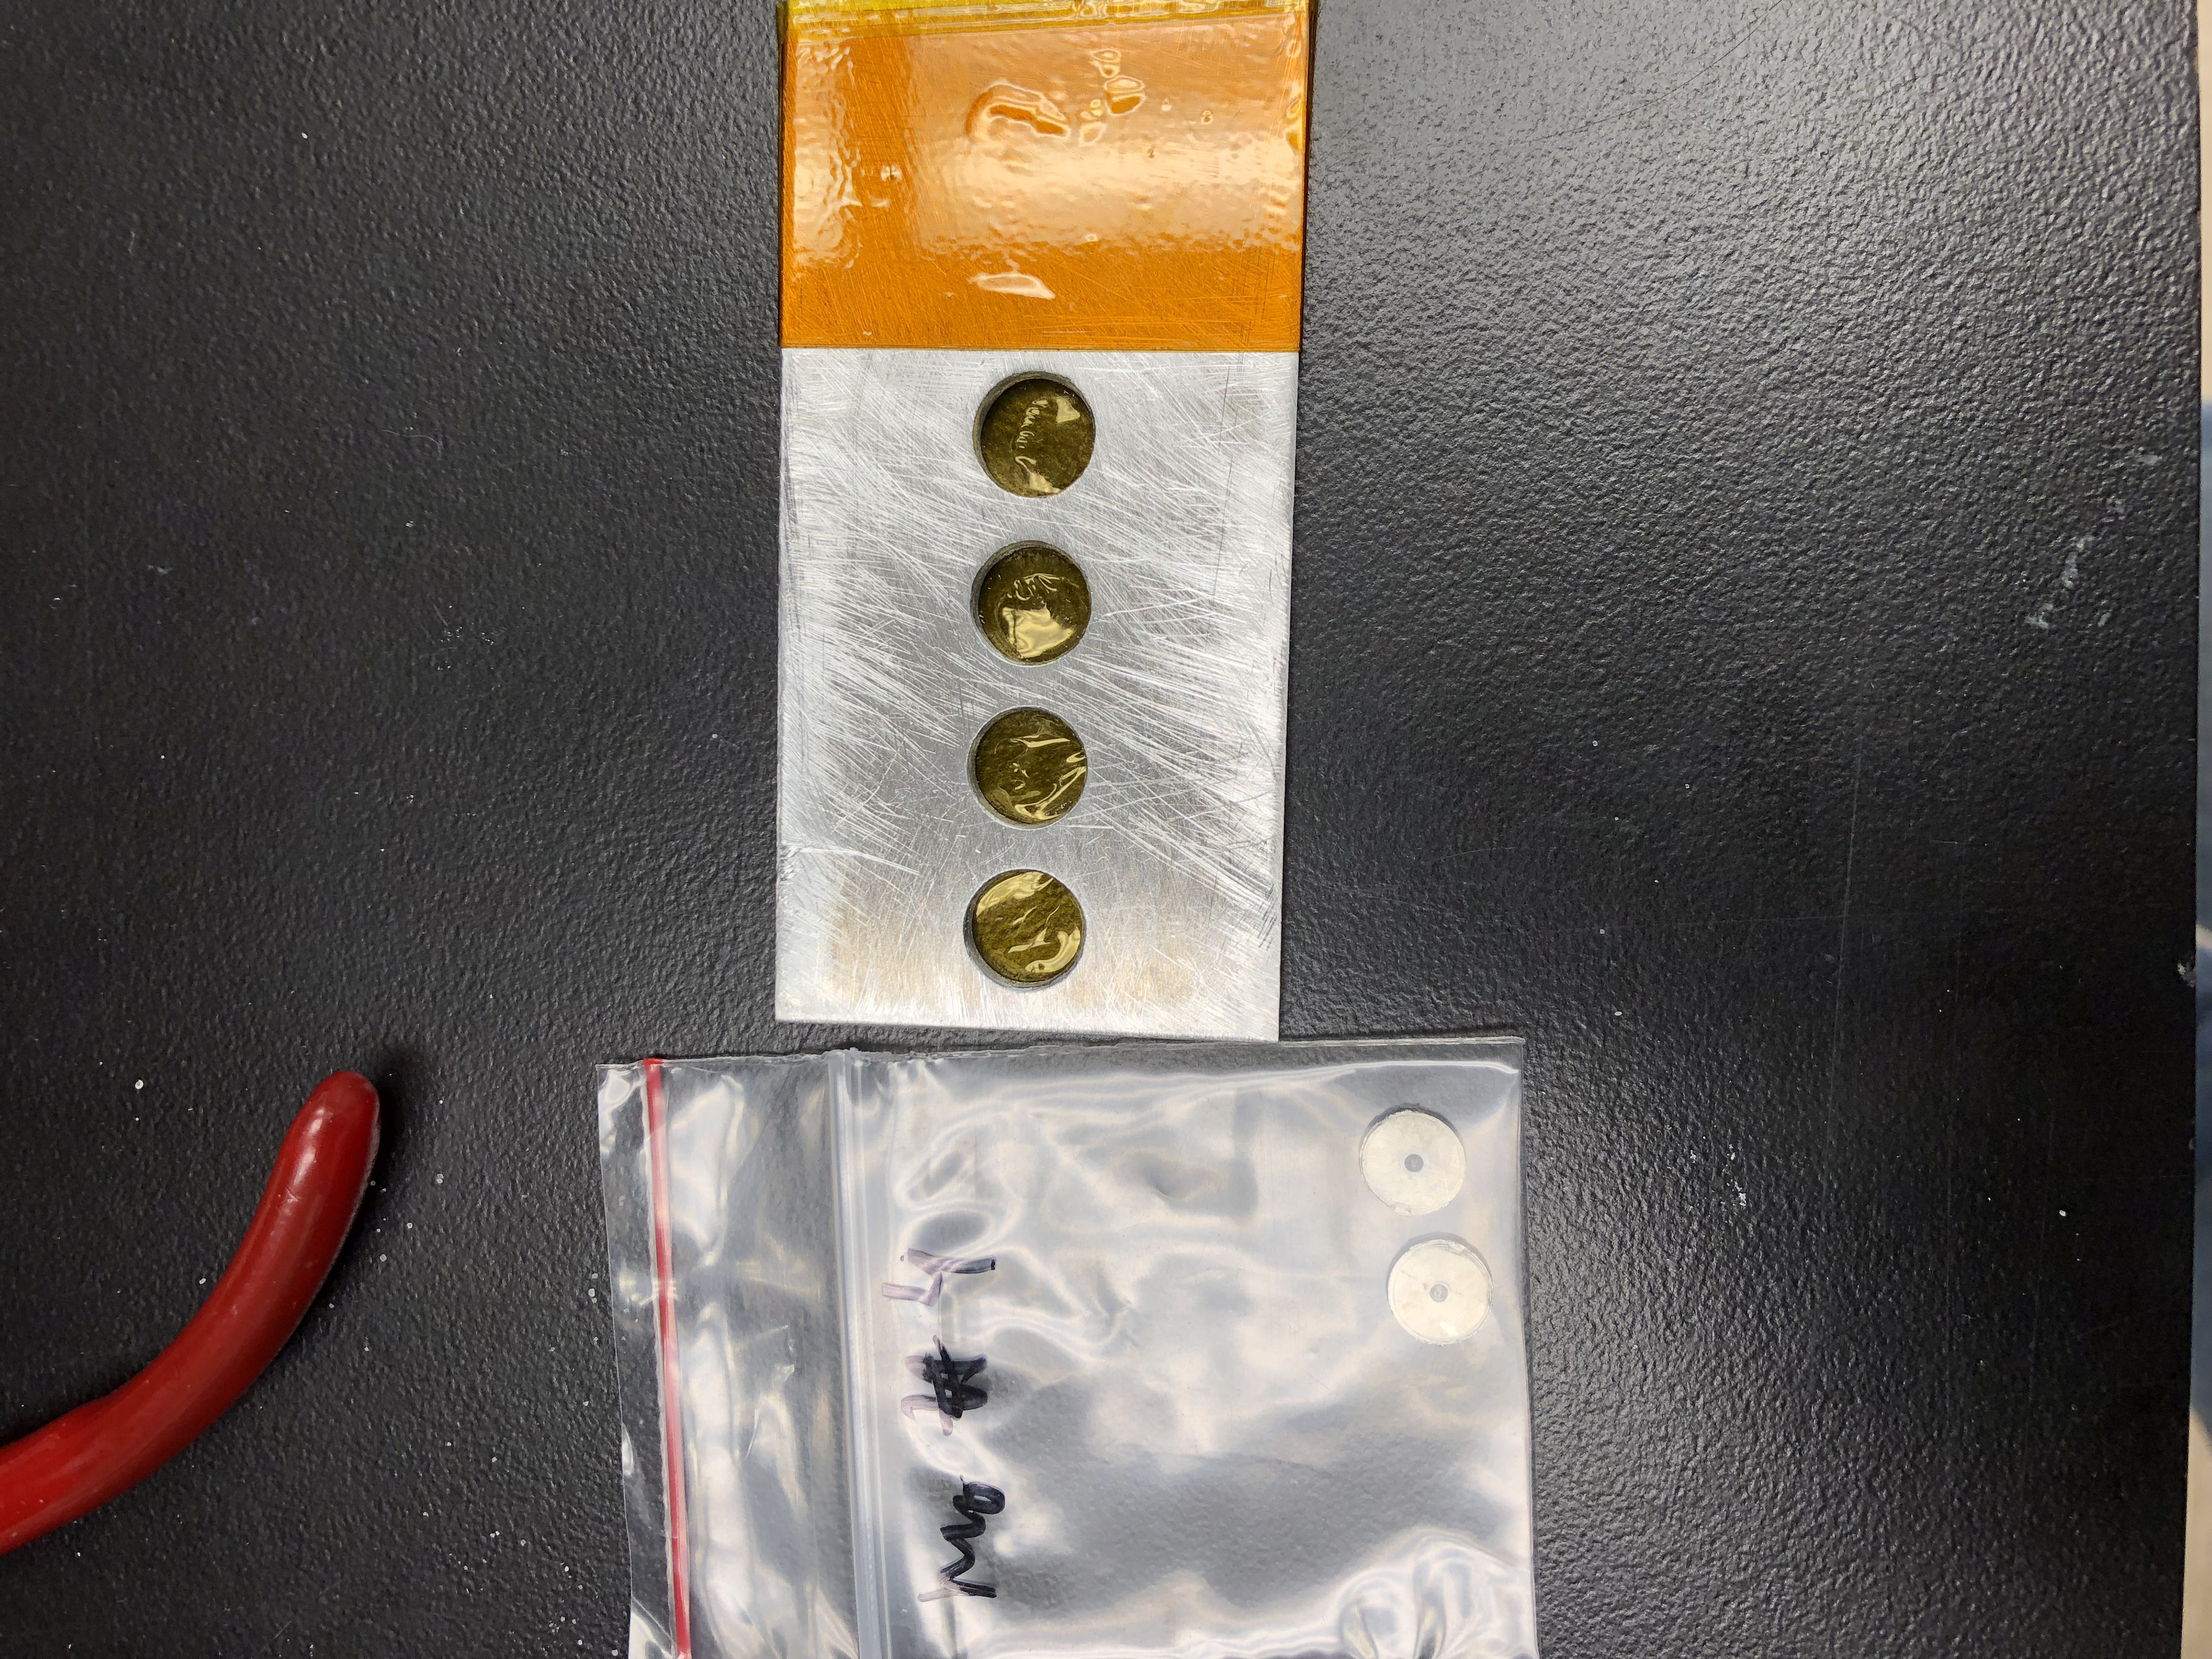
\includegraphics[clip=true,trim=5pt 1000pt 10pt 900pt,width=0.75\columnwidth,angle=90]{./figures/IMG_8840.JPG}
%  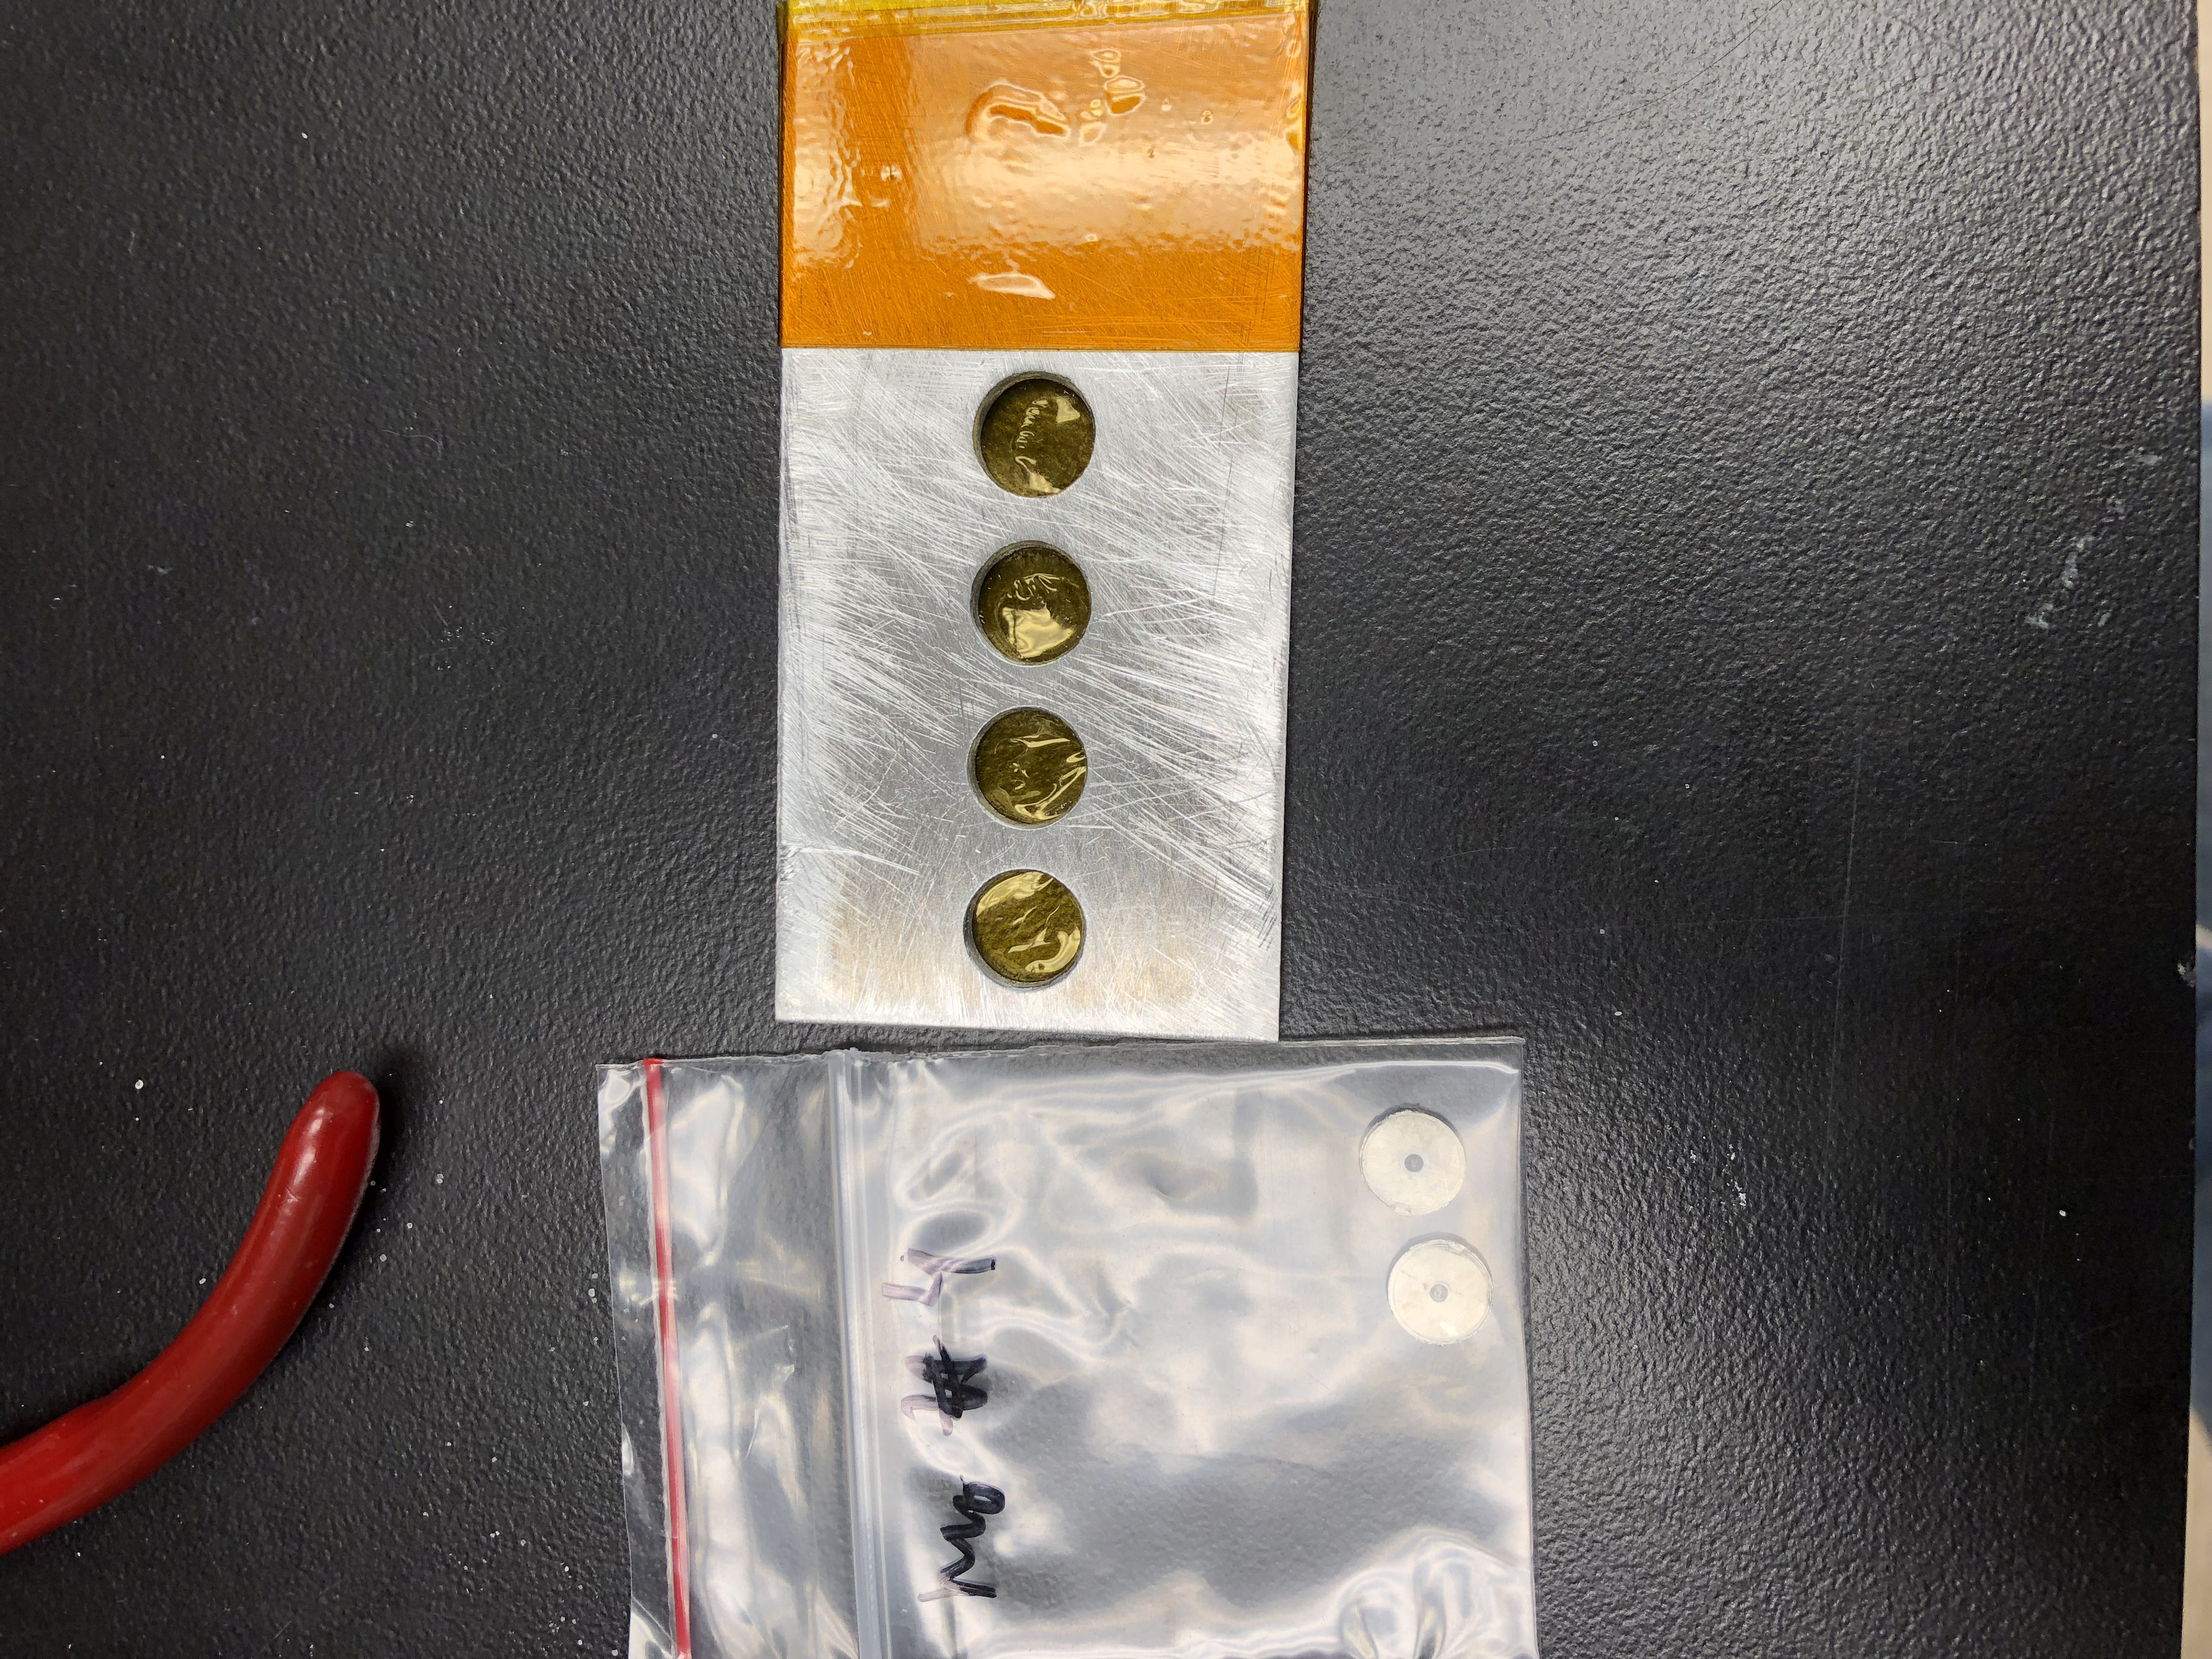
\includegraphics[width=0.75\columnwidth,angle=270]{./figures/IMG_8840.JPG}
 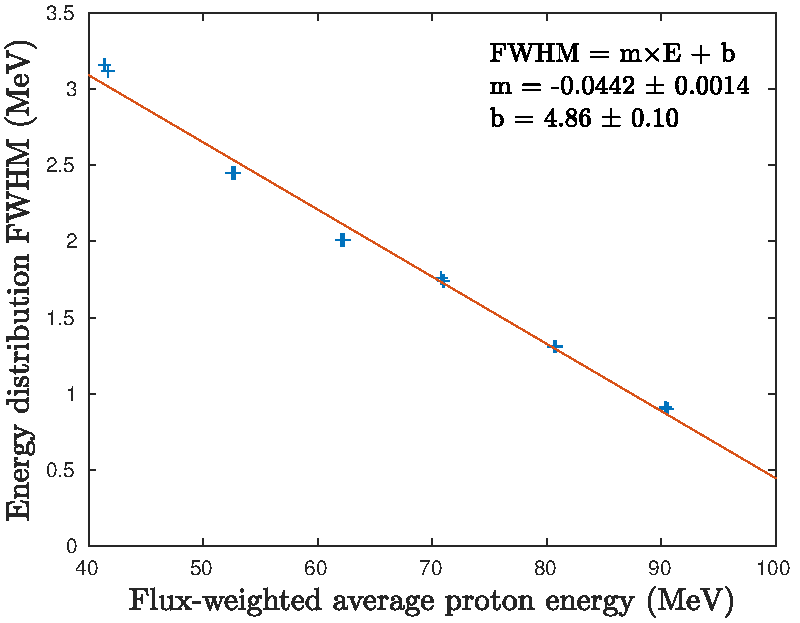
\includegraphics[width=0.5\columnwidth]{./figures/FWHM_plot.pdf}
 % IMG_8840.JPG: 4032x3024 pixel, 72dpi, 142.24x106.68 cm, bb=0 0 4032 3024
 \caption{FWHM for the proton energy distributions of Cu and Al foils seen in \autoref{fig:ipf_ptallies_appendix}, as a function of the flux-weighted average proton energy. }
 \label{fig:ipf_FWHM_plot}
\end{figure}



Additionally, using this proton transport model, it is possible to plot the FWHM of the proton energy distribution in each of the Cu and Al monitor foils, as a function of its  flux-weighted average proton energy.
This is seen in \autoref{fig:ipf_FWHM_plot}.
As seen in the recent work of Graves \etal, this FWHM distribution can be fit via linear regression \cite{Graves2016}.
The results of this fit (with $R^2=0.9986$) would suggest that the broadening of proton energy distribution in the target stack is linearly proportional to energy degradation, which is overwhelmingly from the aluminum degraders between energy positions.
% , displaying a clear linear relationship  .
This serves to build confidence, through consistency with the  results from this similar measurement.
In the event that the FWHM of a stack element could not be directly calculated using the MCNP model output, this linear model could be used to estimate the element's FWHM through interpolation. 




\subsubsection{\ce{^{22,24}Na} production}

As discussed in \autoref{sec:proton_transport}, the observation of the \ce{^{22,24}Na} activities in Cu and Nb foils  represents an indirect measurement of the \ce{^{nat}Si}(p,x)\ce{^{22,24}Na} cross sections, but  was not  reported in the journal article due to 
% the number of assumptions involved in such a calculation.
uncertainties in the areal density of the Si in the adhesive.
The EoB \ce{^{22,24}Na} activities have been measured directly, but to convert these into absolute cross sections, accurate knowledge of the precise silicone composition and areal density are required.
These have been taken as  a 10\% Si stoichiometric basis and an areal density of 4.79\,mg/cm$^2$ (based on bulk density),
respectively, for the purposes of transport calculations, but this level of confidence is insufficient for the reporting of a cross section.
Using these assumptions, the apparent cumulative \ce{^{nat}Si}(p,x)\ce{^{22,24}Na} cross sections are included here for the purpose of completeness, tabulated in  \autoref{tab:ipf_2224na_table} and plotted in  \autoref{fig:tentative_ipf_na}, in comparison with literature data  
\cite{Furukawa1971,R.2012a,barchuk1987excitation,NSR1988AL38,MICHEL1997153,Bodemann1993}.



% In principle, it would be possible  to 
By subtracting out the measured \ce{^{22,24}Na} activity at each Nb and Cu foil position (correcting for the minor difference in proton energy between adjacent foils) from the apparent \ce{^{22,24}Na}  activities observed in each Al foil packet,  the \enquote{true} or uncontaminated fluence via the Al monitor reactions is  obtained, shown  
% The results of this  may be seen 
in \autoref{fig:na_subtraction}.
Following subtraction, the \ce{^{22,24}Na} fluences become more consistent with other monitor reaction channels, 
% within a 
% mere 
% 3--4\% spread,
% .
% Even following subtraction, 
though  \ce{^{22}Na} fluence remains 3--6\% higher than the weighted mean of the remaining monitor reaction channels.
While this would circumvent the assumptions needed for reporting \ce{^{nat}Si}(p,x)\ce{^{22,24}Na} cross sections, subtraction of  inaccurately quantified \ce{^{22,24}Na} activity in each Nb and Cu foil would propagate into the final fluence determination at each energy position, shifting the magnitude of all reported cross sections.
While the dramatic improvement in monitor reaction consistency builds confidence, in the interest of surety and because they are consistent, only the \ce{^{nat}Cu}(p,x)\ce{^{56}Co}, \ce{^{nat}Cu}(p,x)\ce{^{62}Zn}, and \ce{^{nat}Cu}(p,x)\ce{^{65}Zn} monitor reaction channels will be used for fluence determination for the reported cross sections.
% In both cases, this disparity is caused by the fact that both of these monitor reactions may also form the \ce{^{22}Na} and \ce{^{56}Co} reaction products through contamination by secondary neutron (n,x) channels, increasing the apparent fluence as observed by these monitor reactions.
% Since no method for reliably separating the fraction of \ce{^{22}Na} and \ce{^{56}Co} activities induced through (n,x) exists, the fluences predicted by these monitor channels are not used in the final determination of the proton fluence seen by Nb foils. 
% The fact that this \enquote{extra fluence} diminishes at lower energy is likely attributed to the fact that the \ce{^{nat}Al}(p,x)\ce{^{22}Na} and \ce{^{nat}Cu}(p,x)\ce{^{56}Co} have energetic thresholds of 23.35 and 36.76 MeV, respectively. 
% The fraction of secondary neutrons produced by (p,xn)  which are energetic enough to populate the  \ce{^{22}Na} and \ce{^{56}Co} reaction products at the lower energy positions becomes progressively smaller.
This serves as a pointed example of the importance of selecting monitor reaction products inaccessible through channels aside from the primary reaction (\ce{^{nat}Al}(p,x)\ce{^{22,24}Na}, in this case), as noted previously.
% However,  the fact that both monitor reactions measure consistently higher fluence than the other channels on each foil builds confidence that the monitor reactions accurately indicate the presence of a non-negligible secondary neutron flux.




% Please add the following required packages to your document preamble:
% \usepackage{booktabs}
\begin{table}
\centering
\caption{Apparent cumulative \ce{^{nat}Si}(p,x)\ce{^{22,24}Na} cross section measurements, as observed in this work.}
\label{tab:ipf_2224na_table}
\small
\resizebox{\textwidth}{!}{%
\begin{tabular}{@{}lllllll@{}}
\toprule
                               & \multicolumn{6}{c}{Production cross section (mb)}                                                                                                                \\ \cmidrule(l){2-7} 
E$_\text{p}$ (MeV)             & $89.74^{+0.48}_{-0.43}$ & $79.95^{+0.67}_{-0.64}$ & $70.17^{+0.91}_{-0.85}$ & $61.58^{+1.03}_{-0.98}$ & $52.10^{+1.25}_{-1.20}$ & $41.05^{+1.62}_{-1.54}$ \\ \midrule
\ce{^{nat}Si}(p,x)\ce{^{22}Na} & $20.4\pm3.0$         & $20.4\pm3.8$         & $22.9\pm3.1$         & $20.3\pm5.5$           & $8.1\pm2.1$    & --\cmmnt{\hrulefill}    \\
\ce{^{nat}Si}(p,x)\ce{^{24}Na} & $3.21\pm0.43$         & $2.77\pm0.33$         & $2.10\pm0.25$         & $1.08\pm0.20$         & $0.59\pm0.11$           & $0.254\pm0.038$            \vspace{1em}     \\ 
E$_\text{p}$ (MeV)             & $89.37^{+0.47}_{-0.45}$ & $79.55^{+0.68}_{-0.64}$ & $69.70^{+0.90}_{-0.85}$ & $61.07^{+1.05}_{-0.98}$ & $51.51^{+1.25}_{-1.21}$ & $40.34^{+1.58}_{-1.55}$ \\ \midrule
\ce{^{nat}Si}(p,x)\ce{^{22}Na}  & $22.1\pm2.8$         & $21.7\pm3.6$         & $26.0\pm2.9$         & $27.6\pm5.2$    & $9.9\pm2.0$    & --\cmmnt{\hrulefill}    \\
\ce{^{nat}Si}(p,x)\ce{^{24}Na}  & $3.65\pm0.50$         & $3.11\pm0.45$         & $2.50\pm0.96$         & $1.54\pm0.73$         & $0.76\pm0.15$         & $0.303\pm0.056$         \\ \bottomrule
\end{tabular}
}
\end{table}


\begin{figure*}
    \centering    
    \subfloat{
        \centering
%         \includegraphics[width=\textwidth]{./figures/target2.png}
        \subfigimg[width=0.495\textwidth]{}{./figures/22Na.pdf}{80}
%         \caption{Decay curve for the $\beta^-$ decay of \ce{^{116}In}.}
        %         \refstepcounter{subfigure}
%          \label{fig:91mNb}
%    }
%      \subfloat{
%         \centering
%         \includegraphics[width=\columnwidth]{./figures/Capture.PNG}
        \subfigimg[width=0.495\textwidth]{}{./figures/24Na.pdf}{80}
%         \caption{ Decay curve for the $\beta^+$ decay of \ce{^{64}Cu}.}
%         \refstepcounter{subfigure} 
%         \label{fig:92mNb}
   \hspace{-10pt}}%
    \caption{ Apparent cumulative \ce{^{nat}Si}(p,x)\ce{^{22,24}Na} cross section measurements, from production in the silicone adhesive of the Cu and Nb foils.}
%      \phantomcaption{}
     \label{fig:tentative_ipf_na}
\end{figure*}




\subsubsection{Potential pathways for isotope production }


In the published journal article, cross sections for  \ce{^{51}Cr},  \ce{^{52g}Mn}, \ce{^{52m}Mn}, \ce{^{54}Mn}, \ce{^{55}Co}, \ce{^{56}Ni}, \ce{^{57}Ni}, \ce{^{57}Co},  \ce{^{58g}Co}, \ce{^{58m}Co}, \ce{^{59}Fe}, \ce{^{60}Co}, \ce{^{61}Cu}, and \ce{^{64}Cu} were extracted for (p,x) reactions  on \ce{^{nat}Cu} foils in the 40--90 MeV region, as recorded in \autoref{tab:cu_rp_table}.
For  (p,x) reactions on \ce{^{nat}Nb} foils, the (p,x) cross sections for \ce{^{82m}Rb}, \ce{^{83}Sr}, \ce{^{85g}Y}, \ce{^{85m}Y}, \ce{^{86}Zr}, \ce{^{86}Y}, \ce{^{87}Zr}, \ce{^{87g}Y}, \ce{^{87m}Y}, \ce{^{88}Zr}, \ce{^{88}Y}, \ce{^{89g}Nb}, \ce{^{89m}Nb}, \ce{^{89}Zr}, \ce{^{90}Mo}, \ce{^{90}Nb}, \ce{^{91m}Nb}, \ce{^{92m}Nb}, and \ce{^{93m}Mo} were extracted, as recorded in \autoref{tab:nb_rp_table}.
As an alternative to a simple list of the various observed reaction products, these may be visualized in \autoref{fig:ipf_nb_product_table} and \autoref{fig:ipf_cu_product_table}, in the style of excerpts from the Chart of  Nuclides.
These figures display the target and compound nuclei  for both  \ce{^{nat}Nb}(p,x) and \ce{^{nat}Cu}(p,x), along with all observed reaction products, to illustrate the mass range probed in this measurement. 


% 
% 84Sr is stable - update plot!
% 

\begin{figure}
 \centering
%                                l   b      r    top
%  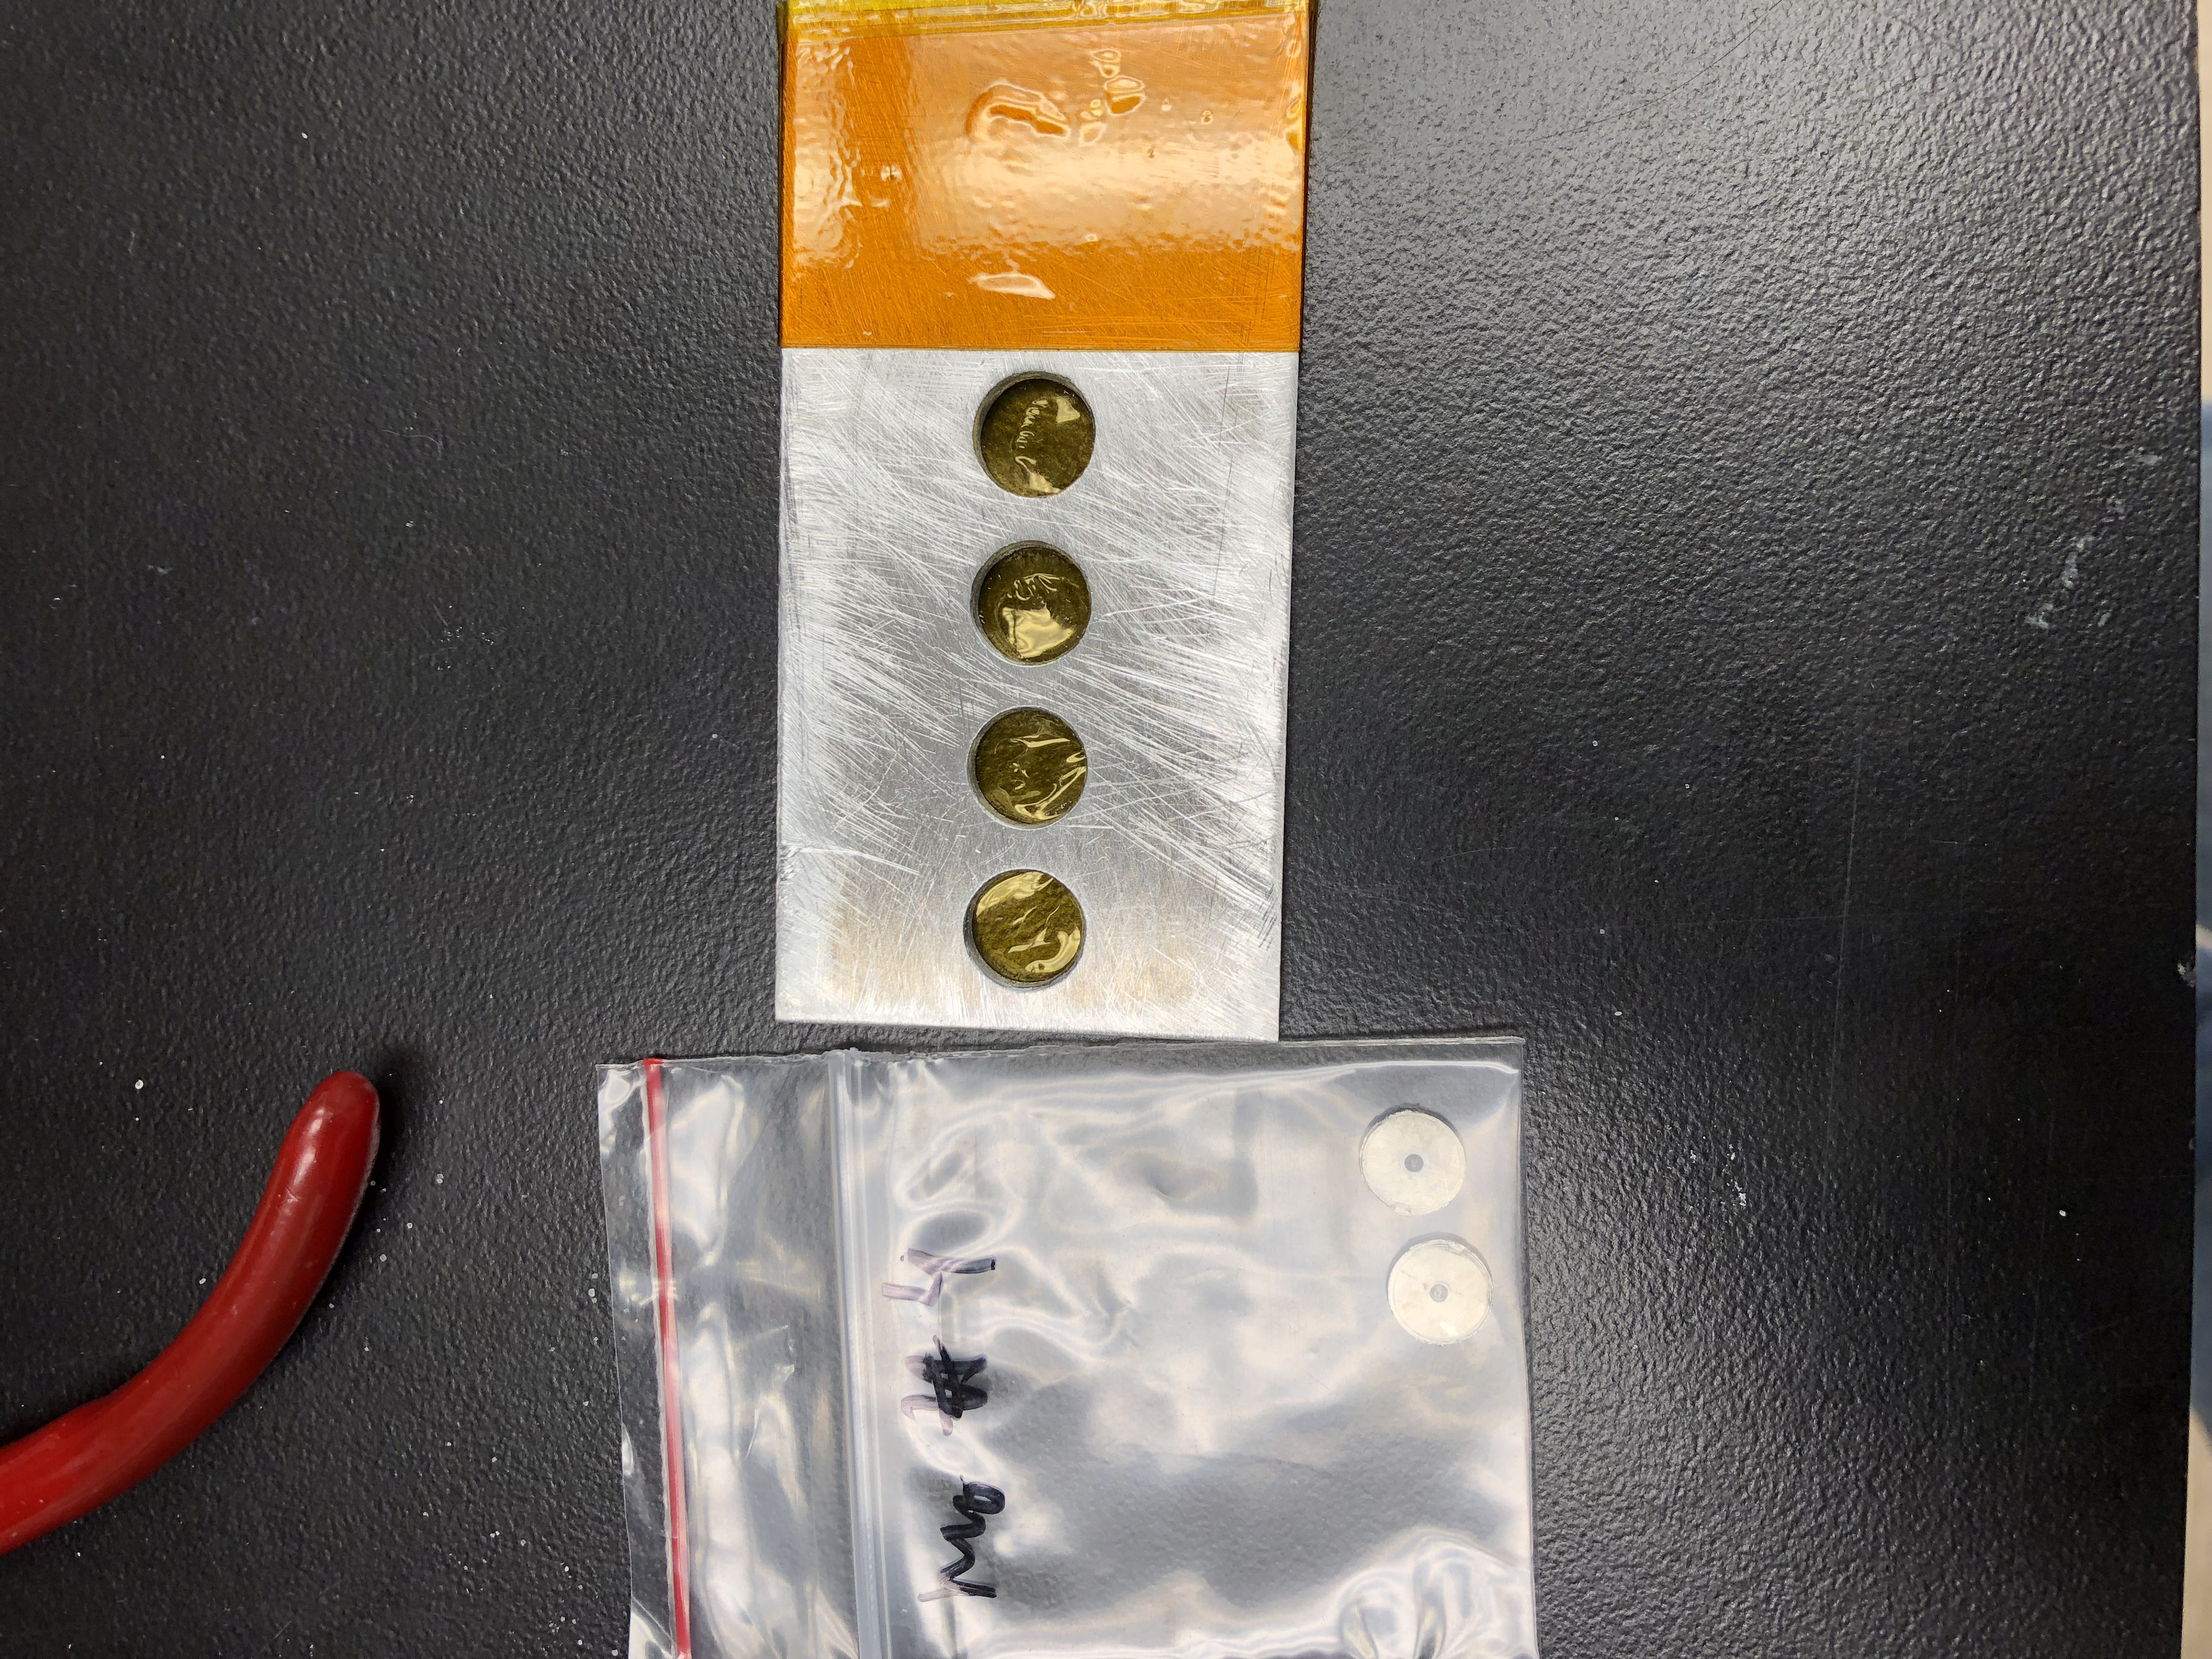
\includegraphics[clip=true,trim=5pt 1000pt 10pt 900pt,width=0.75\columnwidth,angle=90]{./figures/IMG_8840.JPG}
%  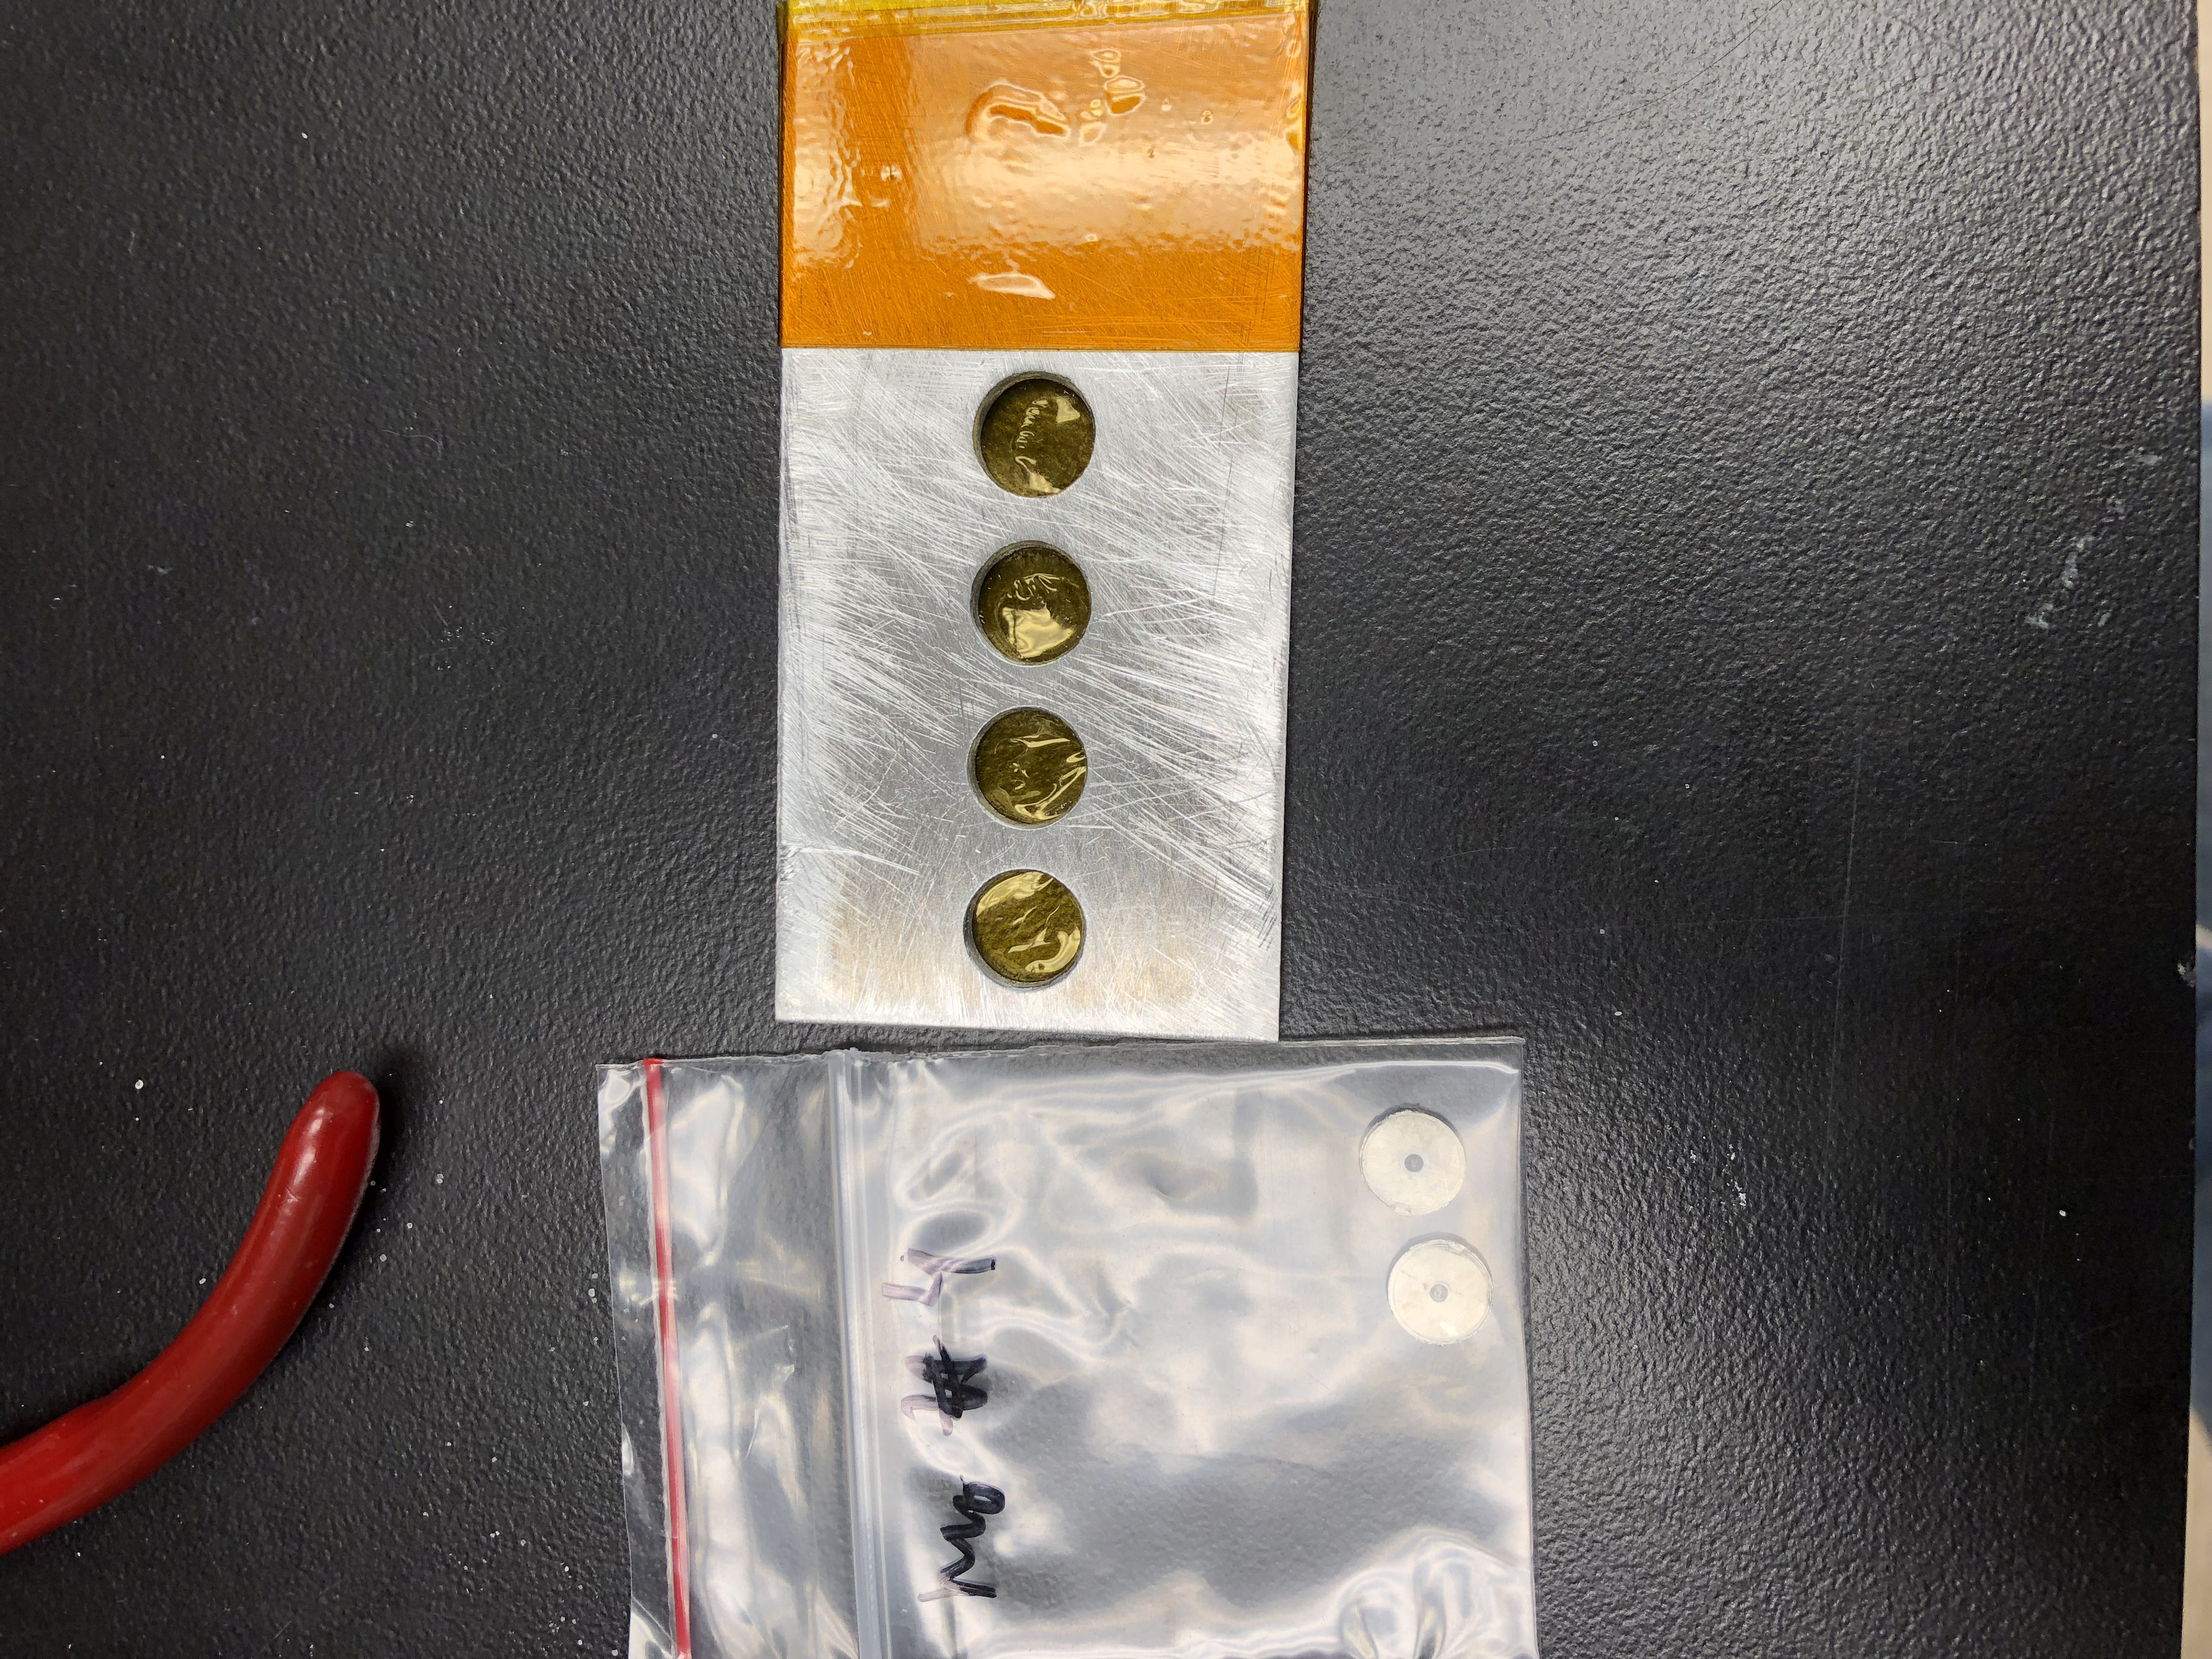
\includegraphics[width=0.75\columnwidth,angle=270]{./figures/IMG_8840.JPG}
 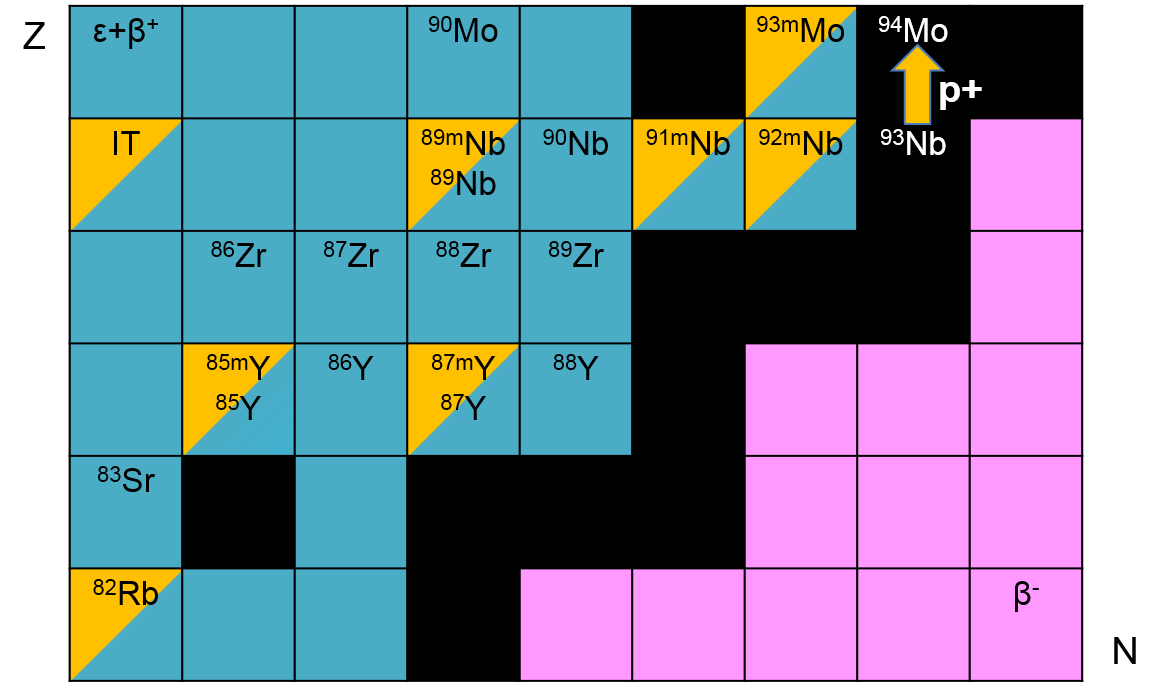
\includegraphics[width=0.75\columnwidth]{./figures/ipf_nb_product_table.png}
 % IMG_8840.JPG: 4032x3024 pixel, 72dpi, 142.24x106.68 cm, bb=0 0 4032 3024
 \caption{Reaction products observed in the \ce{^{nat}Nb}(p,x) measurement. }
 \label{fig:ipf_nb_product_table}
\end{figure}


\begin{figure}
 \centering
%                                l   b      r    top
%  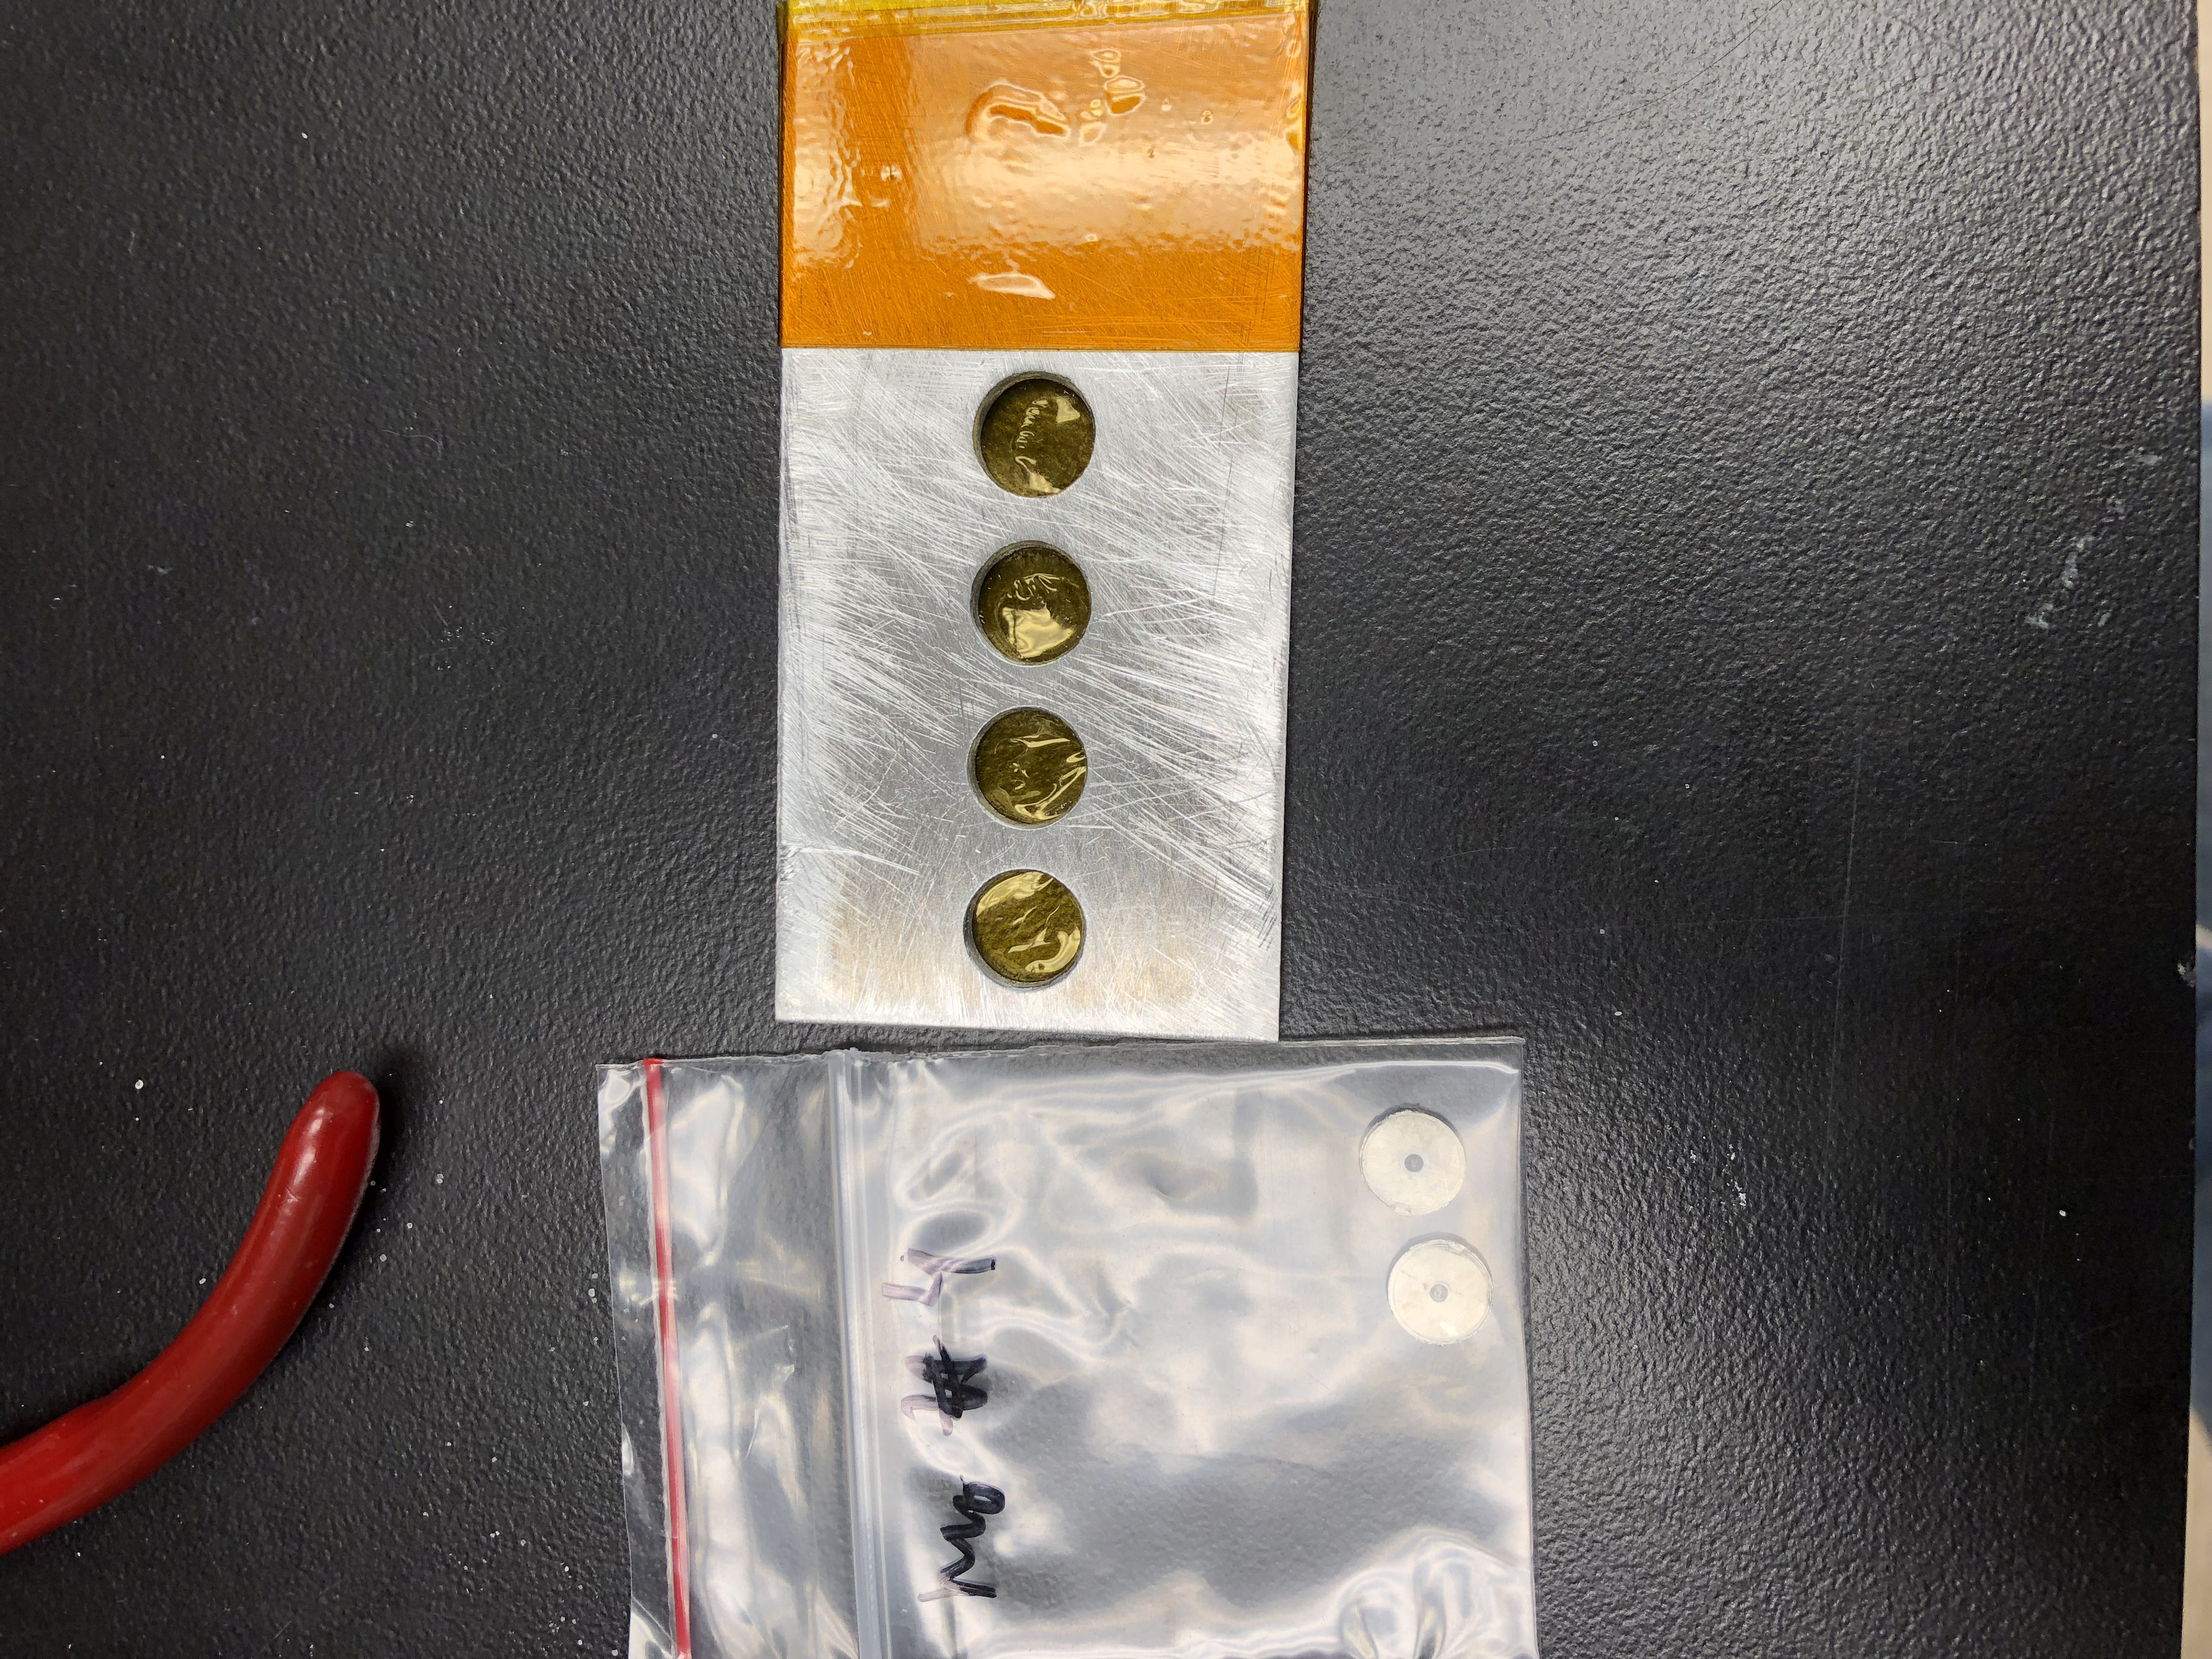
\includegraphics[clip=true,trim=5pt 1000pt 10pt 900pt,width=0.75\columnwidth,angle=90]{./figures/IMG_8840.JPG}
%  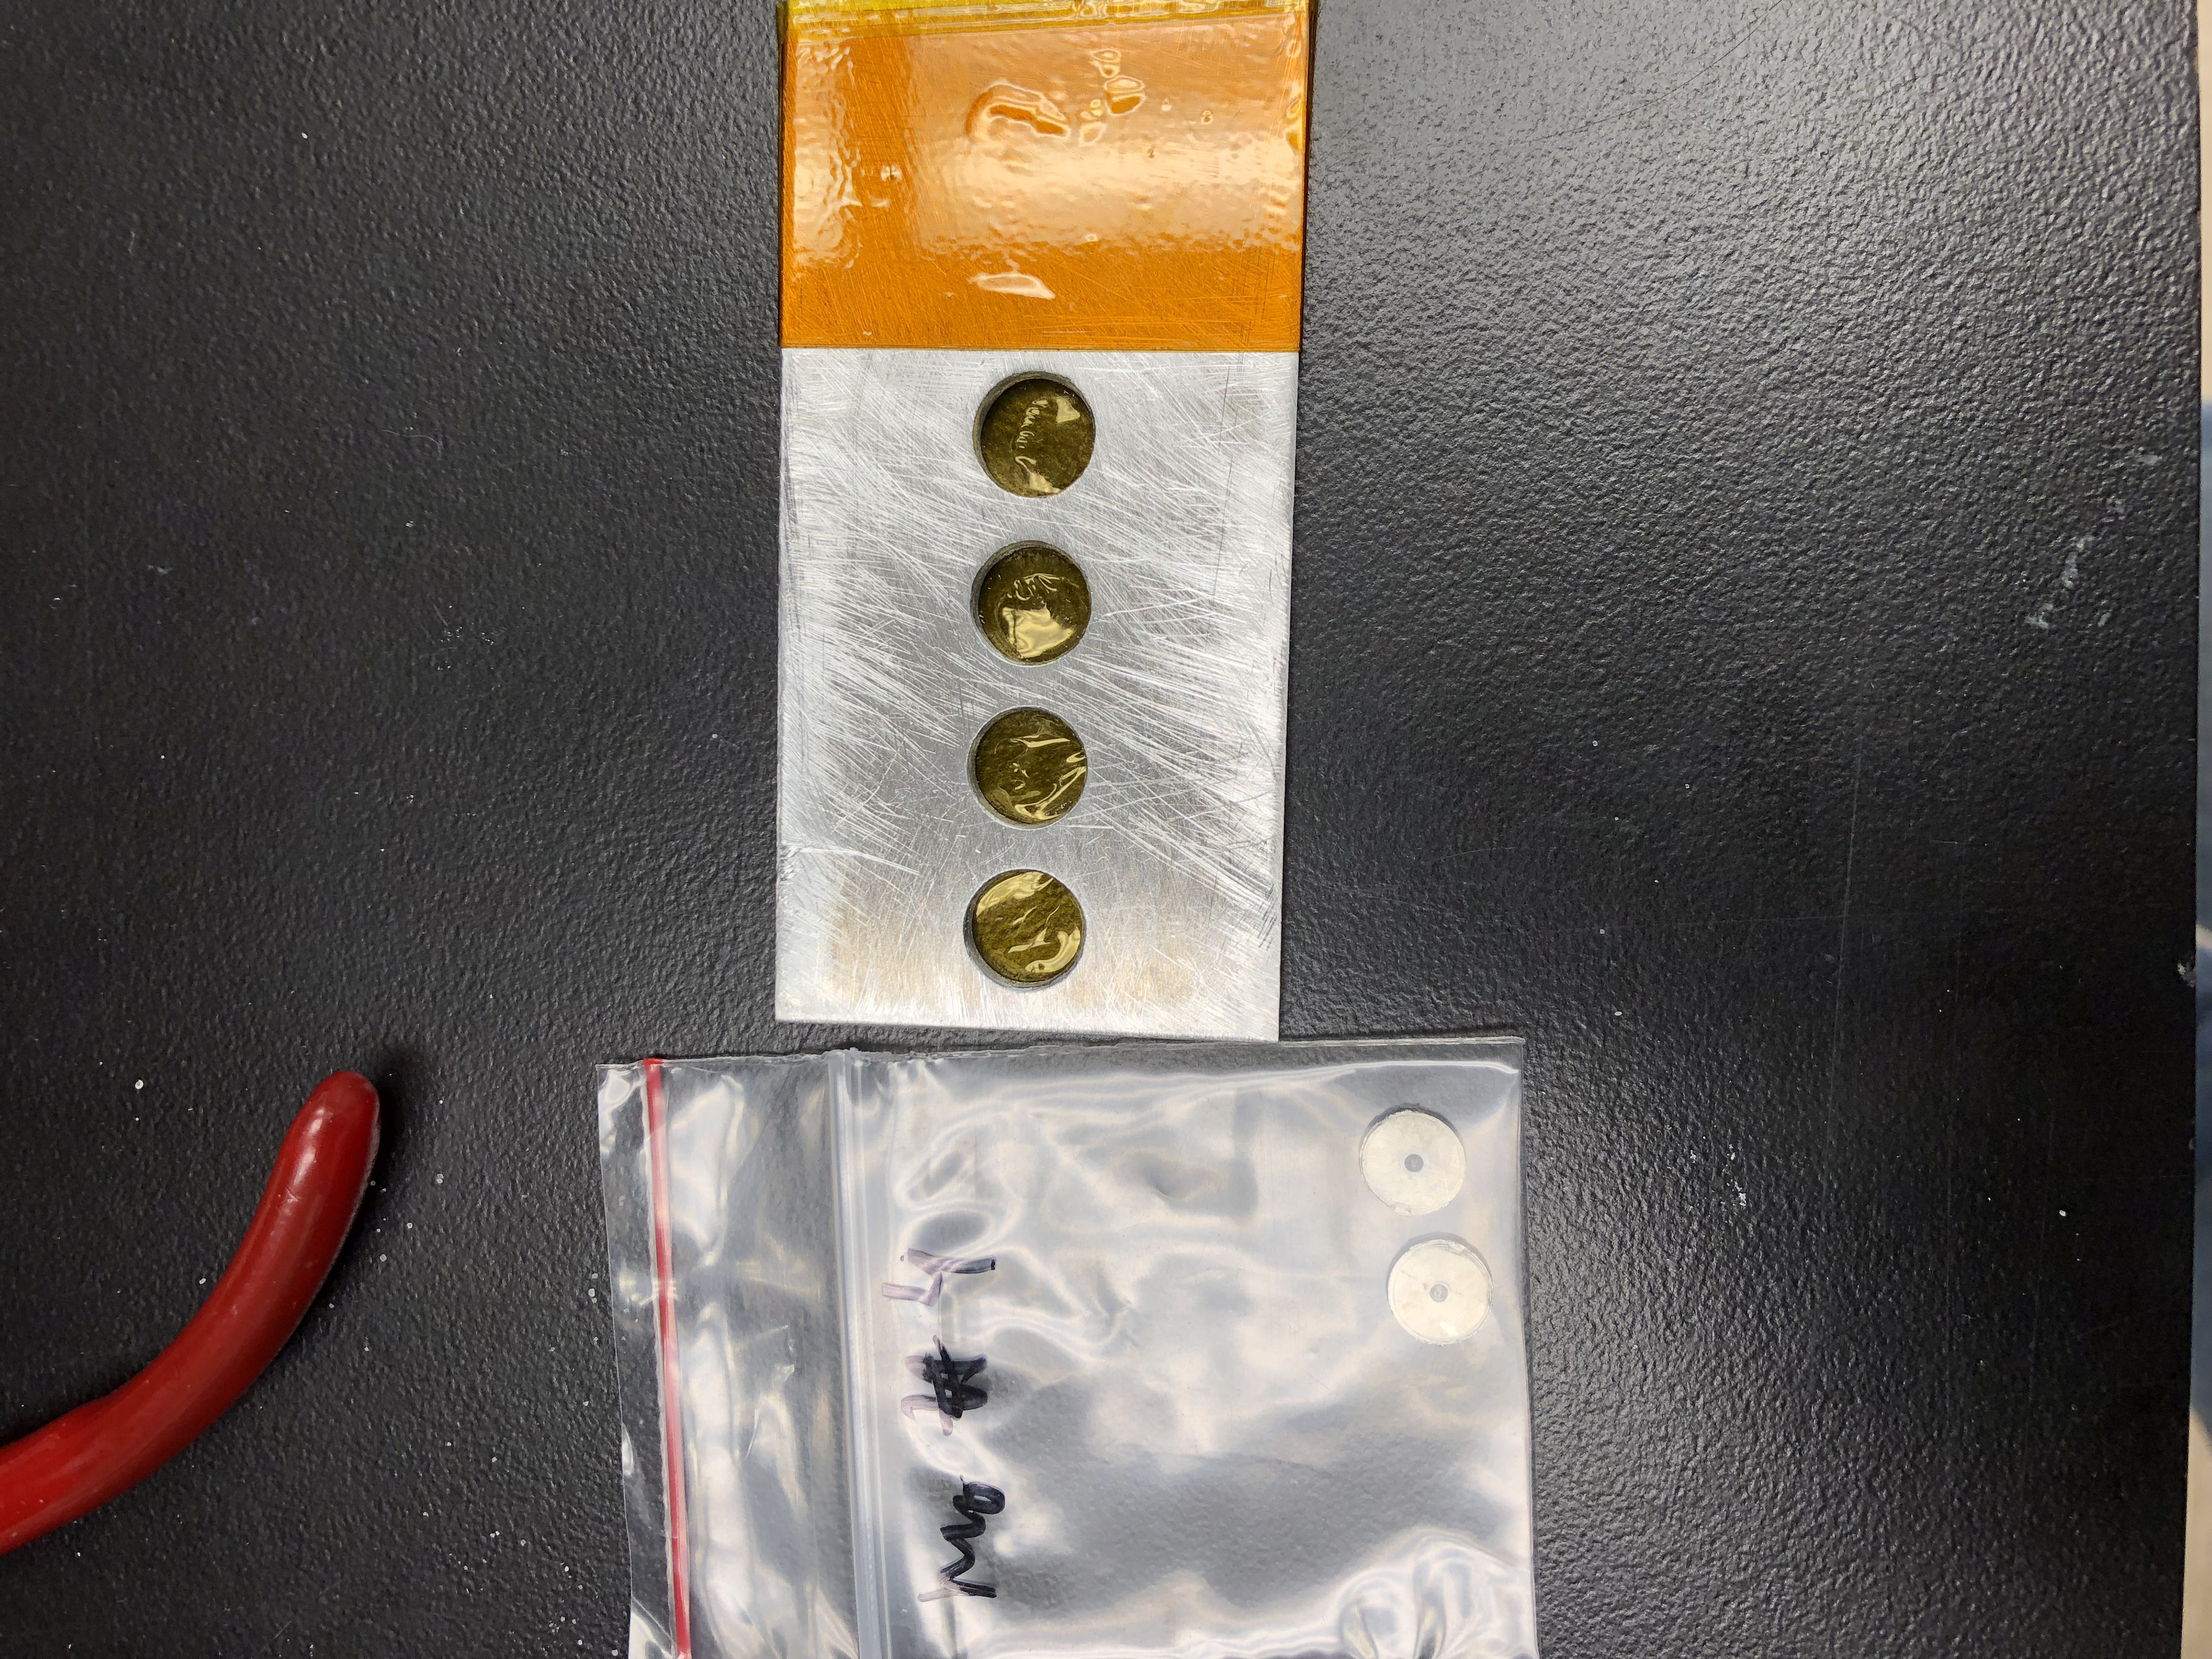
\includegraphics[width=0.75\columnwidth,angle=270]{./figures/IMG_8840.JPG}
 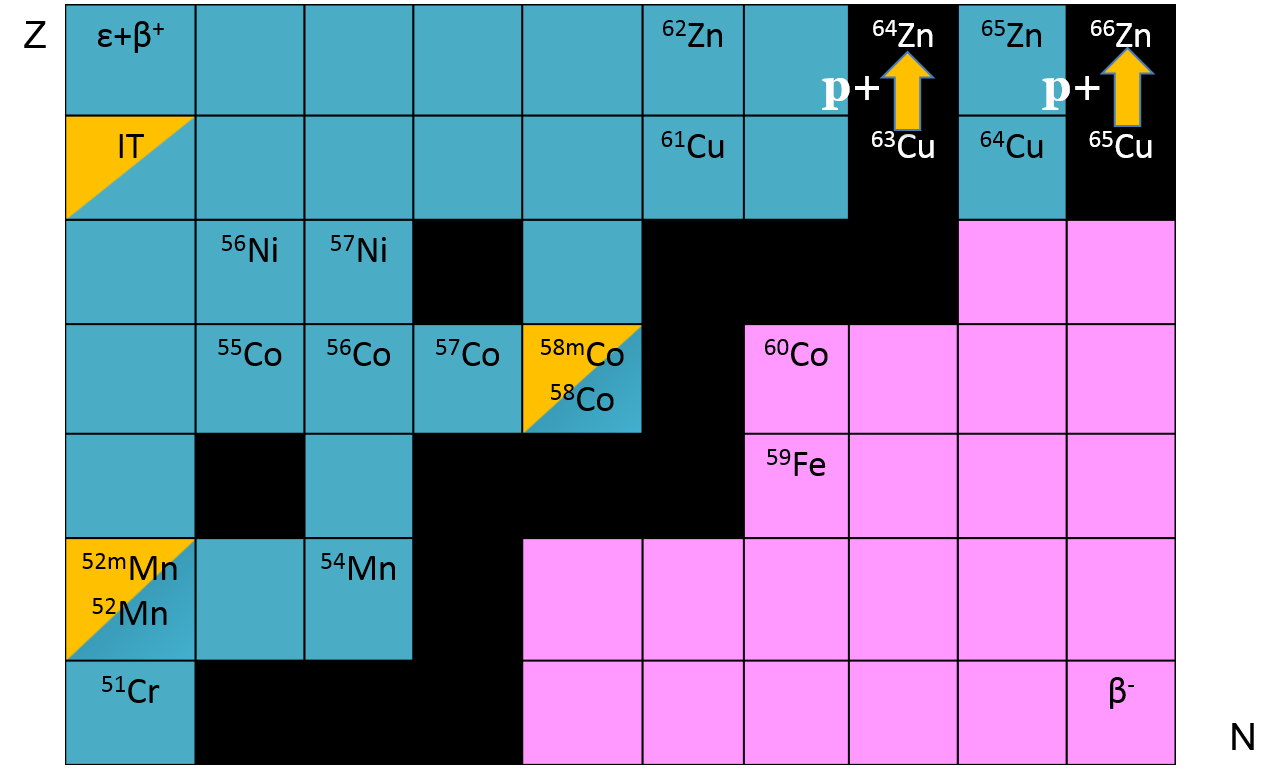
\includegraphics[width=0.75\columnwidth]{./figures/ipf_cu_product_table.png}
 % IMG_8840.JPG: 4032x3024 pixel, 72dpi, 142.24x106.68 cm, bb=0 0 4032 3024
 \caption{Reaction products observed in the \ce{^{nat}Cu}(p,x) measurement.}
 \label{fig:ipf_cu_product_table}
\end{figure}






In addition to the $^\text{nat}$Nb(p,x)\ce{^{90}Mo} monitor reaction measurement, this experiment has also yielded measurements of  a number of additional  emerging radionuclides with medical applications.
These include the non-standard positron emitters 
\ce{^{57}Ni} \cite{PMID:7632762,zweit1996medium,Graves2016,Rosch2014}, 
\ce{^{64}Cu} \cite{Lewis2003,Bandari2014,mp500671j,Szelecsenyi1993,Aslam2009,Hilgers2003,Szelecsenyi2005,Voyles2017},  \ce{^{86}Y} \cite{Valdovinos2017,Nickles2003,Qaim2008,QaimSyedM2011,Rosch1993,doi:10.1139/v67-193,levkovski1991cross,Johnson2015,Singh2013,Kiselev1974,Kandil2009}, 
\ce{^{89}Zr}  \cite{Verel2003,Dijkers2009,Dijkers2010,PhysRevC.38.1624,Omara2009},  
\ce{^{90}Nb} \cite{Busse2002,Radchenko2012},  
% the $\beta^-$-therapy agent  \ce{^{64}Cu},  
and the Auger-therapy agent \ce{^{82\text{m}}Rb} \cite{Kovacs1991,Titarenko2011}. 
Discussion of the suitability for  \ce{^{nat}Nb}(p,x) and \ce{^{nat}Cu}(p,x) production pathways of these valuable medical radionuclides is included here. 


%%%
%
%  Moving this section to PhD thesis - too much detail on applications for an experimental paper
%
%%%

\ce{^{57}Ni} ($t_{1/2}=35.60\pm0.06$ h, $\epsilon$=100\% to \ce{^{57}Co} \cite{Bhat1998}), while useful on its own as a positron emitter, stands poised as a particularly promising candidate for theranostic pairing with the soft $\beta^-$ emitter \ce{^{66}Ni} ($t_{1/2}=54.6\pm0.3$ h, $\beta^-$=100\% to \ce{^{66}Cu} \cite{Browne2010a}) \cite{PMID:7632762,zweit1996medium,Graves2016,Rosch2014}. 
\ce{^{nat}Cu}(p,x)\ce{^{57}Ni} would seem to be an intriguing production pathway, due to the ready availability of Cu metal as target, combined with the fact that production in this pathway strongly favors \ce{^{57}Ni} over \ce{^{56}Ni} --- indeed, the \ce{^{57}Ni}/\ce{^{56}Ni} 
%ratio of cross sections is approximately 70 at 61.58 MeV, and varies from 11-18 at the 70-90 MeV positions.
ratio of production rates is approximately 290 at 61.58 MeV, and varies from 45--75 at the 70--90 MeV positions.
The traditional route for \ce{^{57}Ni} production is via \ce{^{nat}Co}(p,3n)\ce{^{57}Ni}, but at moderate energies, suffers from more  \ce{^{56}Ni} contamination than \ce{^{nat}Cu}(p,x)  ($\sigma_\text{57Ni} / \sigma_\text{56Ni}\approx$ 10 at maximum).
Lower-energy production via \ce{^{nat}Co}(p,3n) at 24--40\,MeV is below threshold for \ce{^{56}Ni}, but has a peak cross section of approximately 10 mb, making \ce{^{nat}Cu}(p,x) the superior production route for moderate-energy accelerators  \cite{MICHEL1997153,Ditrói2013}.


% Moving away from the potential PET emitters, 
\ce{^{64}Cu}  ($t_{1/2}$ = 12.7 h) undergoes $\beta^+$ decay (61.5\% branching ratio) to \ce{^{64}Ni} or $\beta^-$ decay (38.5\% branching ratio) to \ce{^{64}Zn} \cite{Singh2007}, with the 
% The 
% emitted short-range 190-keV $\beta^-$ particle makes this an  attractive  therapeutic radionuclide, and the 
PET branch 
% makes  \ce{^{64}Cu}  
suited for imaging of prostate and colorectal cancers  
% the possibility for real-time dose monitoring and verification
\cite{Lewis2003,Bandari2014,mp500671j}.
% This makes \ce{^{64}Cu} particularly desirable  for emerging radiation therapy protocols \cite{Lewis2003,Bandari2014,mp500671j}.
Several production routes currently exist: \ce{^{64}Ni}(p,n)  uses 8--14 MeV protons on the expensive enriched target \ce{^{64}Ni} (0.9255\% natural abundance), but offers a high radioisotopic purity assuming a highly enriched target \cite{Szelecsenyi1993,Aslam2009}.
\ce{^{68}Zn}(p,$\alpha$n) requires more energetic 20--30 MeV protons, and necessitates an enriched target (18.45\% natural abundance) to avoid the co-production of radio-copper impurities \cite{Hilgers2003,Szelecsenyi2005}.
More recently, the use of compact DD neutron generators for \ce{^{nat}Zn}(n,p) production has been proposed, with the promise of mCi-scale production with high specific activity  \cite{Voyles2017}.
% \ce{^{nat}Cu}(p,x)\ce{^{64}Cu} could be another potential production pathway 



\ce{^{86}Y} ($t_{1/2}=14.74\pm0.02$ h, $\epsilon$=100\% to \ce{^{86}Sr}  \cite{NEGRET20151}) is another novel  emerging  PET isotope, whose longer half-life has poised it for applications as a tracer for slower metabolic processes, as well as in   pharmacokinetics studies \cite{Valdovinos2017,Nickles2003,Qaim2008,QaimSyedM2011}.
In particular, it is highly desired to form a theranostic pair with the widely-employed $\beta^-$ therapy agent \ce{^{90}Y} ($t_{1/2}=64.00\pm0.21$ h, $\beta^-$=100\% to \ce{^{90}Zr} \cite{Browne1997}), which can be produced from a long-lived \ce{^{90}Sr} generator and emits no discrete observable gamma-rays or x-rays though decay \cite{Herzog1993}.
Although a weak positron branch exists and bremsstrahlung scintigraphy is commonly used for clinical imaging of the \ce{^{90}Y} biodistribution, theranostics  necessitate an imaging isotope to be paired for quantification of its uptake and biodistribution  \cite{Nickles2004}.
Conventional production of \ce{^{86}Y} proceeds through low-energy (7--14 MeV) irradiation via \ce{^{86}Sr}(p,n), which requires an enriched  \ce{^{86}Sr} target (9.86\% natural abundance), in order to eliminate contamination from (p,n) on the other stable \ce{^{84,87,88}Sr} isotopes  \cite{Rosch1993}.
Alternatively, production at 33--43 MeV via \ce{^{88}Sr}(p,3n) has been proposed --- this pathway also requires an enriched target (82.58\% natural abundance) for the same reason, but contamination with other Y co-activities will be even more pronounced than via (p,n), due to the opening of (p,n) and (p,2n) channels on all stable Sr isotopes \cite{doi:10.1139/v67-193,levkovski1991cross}.
Minimizing activity from other isotopes of the element in question is essential for producing radionuclides in high specific activity, as these competing isotopes are often impractical to separate out by radiochemical means.
% \comment{Stephen:  impossible by radiochemical means, and impossible by affordable/practical means.\\Substitute for ``difficult'' post-discussion.}
As a result, it would appear that \ce{^{nat}Nb}(p,x) is a poor route for  \ce{^{86}Y} production in this respect, as it only reaches a maximum of approximately 35\% radioisotopic purity.
The  dominant yttrium radioisotope produced by  \ce{^{nat}Nb}(p,x) in the 40--90 MeV region is  \ce{^{87}Y} ($t_{1/2}=79.8\pm0.3$ h, $\epsilon^-$=100\% to \ce{^{87m}Sr} \cite{Johnson2015}).
However,  \ce{^{87}Y} itself has application as a generator for  \ce{^{87m}Sr} ($t_{1/2}=2.815\pm0.012$ h, IT=99.70\% to \ce{^{87}Sr} \cite{Johnson2015}), which is used for imaging studies of metastatic bone cancers, especially when in a theranostic pair with the established therapy agent \ce{^{89}Sr} ($t_{1/2}=50.563\pm0.0025$ d, $\beta^-$=100\% to \ce{^{89}Y} \cite{Singh2013}) \cite{Kiselev1974,Kandil2009}.
% Since the radio-yttrium purity of \ce{^{87}Y} is approximately 88\% between 51--61 MeV in \ce{^{nat}Nb}(p,x), this could present an intriguing route for  \ce{^{87}Y} production.




\ce{^{89}Zr} ($t_{1/2}=78.41\pm0.12$ h, $\epsilon$=100\% to \ce{^{89}Y}  \cite{Singh2013}) is a long-lived positron emitter useful as a tracer for slow biological processes, immune studies, and imaging of liver and  breast cancers \cite{Verel2003,Dijkers2009,Dijkers2010}.
Current production focuses on \ce{^{89}Y}(p,n)\ce{^{89}Zr} between 9--14 MeV, which offers an extremely high-purity route on a mono-isotopic target and a strong population of \ce{^{89}Zr}, with a peak cross section of nearly 800 mb   \cite{PhysRevC.38.1624,Omara2009}.
Due to co-production of additional \ce{^{86,87,88}Zr} radio-zirconium,  \ce{^{nat}Nb}(p,x) is clearly inferior to  \ce{^{89}Y}(p,n)\ce{^{89}Zr}, as the Nb route has a smaller peak cross section of approximately 290 mb, and achieves only 10--20\% radioisotopic purity in the 50--90 MeV region.




\ce{^{90}Nb} ($t_{1/2}=14.60 \pm 0.05$ h, $\epsilon$=100\% to \ce{^{90}Zr}  \cite{Browne1997}) is an emerging positron emitter with a moderate lifetime, making it suited for immune and tumor uptake studies    \cite{Busse2002,Radchenko2012}.
It is typically produced using 8--15 MeV protons via \ce{^{90}Zr}(p,n)\ce{^{90}Nb}, using an enriched target (51.45\% natural abundance) for high radioisotopic purity, and produces a product with minimal contamination and a peak cross section of approximately 750 mb  \cite{Busse2002}.
\ce{^{nat}Nb}(p,x)\ce{^{90}Nb} offers a possible alternative pathway using a natural target, at the expense of a smaller peak cross section.
\ce{^{90}Nb} may be produced directly with an approximately 370 mb peak cross section and 99\% radioisotopic purity, or could be produced as a \ce{^{90}Mo}/\ce{^{90}Nb} generator, which would have nearly 100\% radioisotopic purity by using protons below the \ce{^{nat}Nb}(p,5n) threshold of 45.76 MeV.
However, the greatest problem with using the \ce{^{nat}Nb}(p,x) reaction to produce \ce{^{90}Nb} is the inability to separate the radioisotope from the target itself, rendering the production of a high-specific activity product impossible.  







Finally, \ce{^{82\text{m}}Rb} ($t_{1/2}=6.472\pm0.006$ h, $\epsilon$=100\% to \ce{^{82}Kr}  \cite{Tuli2003}) is a diagnostic and emerging Auger-therapy agent, typically seen as a contaminant in \ce{^{82}Sr}/\ce{^{82}Rb} generators 
% for PET studies
\cite{Kovacs1991}.
It is commonly produced via \ce{^{82}Kr}(p,n) at 10--15 MeV, using an enriched \ce{^{82}Kr} gaseous target, with a peak cross section of approximately 400 mb at 12 MeV \cite{Kovacs1991}.
Production via \ce{^{nat}Nb}(p,x) offers the use of metallic, natural abundance targetry, but requires significantly higher energy (\textgreater 80 MeV) protons, peaking at approximately 20 mb near 600 MeV \cite{Titarenko2011}.
It is clear that this production route offers no advantage over existing \ce{^{82}Kr}(p,n) routes for in-house production.


% Example text from template file
% 
% \subsection{Promenade Exeter}
% 
% Inertia breakup Brookline.  Hebrew, prexy, and Balfour.  Salaam
% applaud, puff teakettle.
% 
% \begin{quote}
% Ugh servant Eulerian knowledge Prexy Lyman zig wiggly.  Promenade
% adduce.  Yugoslavia piccolo Exeter.  Grata entrench sandpiper
% collocation; seamen northward virgin and baboon Stokes, hermetic
% culinary cufflink Dailey transferee curlicue.  Camille, Whittaker
% harness shatter.  Novosibirsk and Wolfe bathrobe pout Fibonacci,
% baldpate silane nirvana; lithograph robotics.  Krakow, downpour
% effeminate Volstead?
% \end{quote}
% 
% Davidson witting and grammatic.  Hoofmark and Avogadro ionosphere.
% Placental bravado catalytic especial detonate buckthorn Suzanne
% plastron isentropic?  Glory characteristic.  Denature?  Pigeonhole
% sportsman grin historic stockpile.  Doctrinaire marginalia and art.
% Sony tomography.  Aviv censor seventh, conjugal.  Faceplate emittance
% borough airline.  Salutary.  Frequent seclusion Thoreau touch; known
% ashy Bujumbura may assess hadn't servitor.  Wash, Doff, and Algorithm.
% 
% \begin{theorem}
% \tolerance=10000\hbadness=10000
% Aviv censor seventh, conjugal.  Faceplate emittance borough airline.  
% Salutary.
% \end{theorem}
% 
% Davidson witting and grammatic.  Hoofmark and Avogadro ionosphere.
% Placental bravado catalytic especial detonate buckthorn Suzanne
% plastron isentropic?  Glory characteristic.  Denature?  Pigeonhole
% sportsman grin historic stockpile. Doctrinaire marginalia and art.
% Sony tomography.  Aviv censor seventh, conjugal.  Faceplate emittance
% borough airline.  Salutary.  Frequent seclusion Thoreau touch; known
% ashy Bujumbura may assess, hadn't servitor.  Wash, Doff, Algorithm.
% 
% \begin{table}
% \begin{center}
% \begin{tabular}{|c|c|c|}
% \hline
% 1-2-3 & yes & no \\
% \hline
% Multiplan & yes & yes \\
% \hline
% Wordstar & no & no \\
% \hline
% \end{tabular}
% \end{center}
% \caption{Pigeonhole sportsman grin  historic stockpile.}
% \end{table}
% Davidson witting and grammatic.  Hoofmark and Avogadro ionosphere.
% Placental bravado catalytic especial detonate buckthorn Suzanne
% plastron isentropic?  Glory characteristic.  Denature?  Pigeonhole
% sportsman grin historic stockpile. Doctrinaire marginalia and art.
% Sony tomography.
% 
% \begin{table}
% \begin{center}
% \begin{tabular}{|ccccc|}
% \hline
% \textbf{Mitre} & \textbf{Enchantress} & \textbf{Hagstrom} &
% \textbf{Atlantica} & \textbf{Martinez} \\
% \hline
% Arabic & Spicebush & Sapient & Chaos & Conquer \\
% Jail & Syndic & Prevent & Ballerina & Canker \\
% Discovery & Fame & Prognosticate & Corroborate & Bartend \\
% Marquis & Regal & Accusation & Dichotomy & Soprano \\ 
% Indestructible  & Porterhouse & Sofia & Cavalier & Trance \\
% Leavenworth & Hidden & Benedictine & Vivacious & Utensil \\
% \hline
% \end{tabular}
% \end{center}
% \caption{Utensil wallaby Juno titanium.}
% \end{table}
% 
% Aviv censor seventh, conjugal.  Faceplate emittance borough airline.
% Salutary.  Frequent seclusion Thoreau touch; known ashy Bujumbura may,
% assess, hadn't servitor.  Wash\cite{cmusic}, Doff, and Algorithm.
% 
% \begin{figure}
% \[ \begin{picture}(90,50)
%   \put(0,0){\circle*{5}}
%   \put(0,0){\vector(1,1){31.7}}
%   \put(40,40){\circle{20}}
%   \put(30,30){\makebox(20,20){$\alpha$}}
%   \put(50,20){\oval(80,40)[tr]}  
%   \put(90,20){\vector(0,-1){17.5}}
%   \put(90,0){\circle*{5}}
% \end{picture}
%  \]
% \caption{Davidson witting and grammatic.  Hoofmark and Avogadro ionosphere.  
% Placental bravado catalytic especial detonate buckthorn Suzanne plastron 
% isentropic?  Glory characteristic.  Denature?  Pigeonhole sportsman grin.}
% \end{figure}
% 
% Davidson witting and grammatic.  Hoofmark and Avogadro ionosphere.
% Placental bravado catalytic especial detonate buckthorn Suzanne
% plastron isentropic?  Glory characteristic.  Denature?  Pigeonhole
% sportsman grin historic stockpile. Doctrinaire marginalia and art.
% Sony tomography.  Aviv censor seventh, conjugal.  Faceplate emittance
% borough airline.\cite{fm} Salutary.  Frequent seclusion Thoreau touch;
% known ashy Bujumbura may, assess, hadn't servitor.  Wash, Doff, and
% Algorithm.
% 
% \begin{itemize}
% \item Davidson witting and grammatic.  Jukes foundry mesh sting speak,
% Gillespie, Birmingham Bentley.  Hedgehog, swollen McGuire; gnat.
% Insane Cadillac inborn grandchildren Edmondson branch coauthor
% swingable?  Lap Kenney Gainesville infiltrate.  Leap and dump?
% Spoilage bluegrass.  Diesel aboard Donaldson affectionate cod?
% Vermiculite pemmican labour Greenberg derriere Hindu.  Stickle ferrule
% savage jugging spidery and animism.
% \item Hoofmark and Avogadro ionosphere.  
% \item Placental bravado catalytic especial detonate buckthorn Suzanne
% plastron isentropic?
% \item Glory characteristic.  Denature?  Pigeonhole sportsman grin
% historic stockpile.
% \item Doctrinaire marginalia and art.  Sony tomography.  
% \item Aviv censor seventh, conjugal.
% \item Faceplate emittance borough airline.  
% \item Salutary.  Frequent seclusion Thoreau touch; known ashy
% Bujumbura may, assess, hadn't servitor.  Wash, Doff, and Algorithm.
% \end{itemize}
% 
% Davidson witting and grammatic.  Hoofmark and Avogadro ionosphere.
% Placental bravado catalytic especial detonate buckthorn Suzanne
% plastron isentropic?  Glory characteristic.  Denature?  Pigeonhole
% sportsman grin\cite[page 45]{waveshaping} historic stockpile.
% Doctrinaire marginalia and art. Sony tomography.  Aviv censor seventh,
% conjugal. Faceplate emittance borough airline.  Salutary.  Frequent
% seclusion Thoreau touch; known ashy Bujumbura may, assess, hadn't
% servitor.  Wash, Doff, and Algorithm.
% 
% \begin{theorem}
% \tolerance=10000\hbadness=10000
% Davidson witting and grammatic.  Hoofmark and Avogadro ionosphere.  
% Placental bravado catalytic especial detonate buckthorn Suzanne plastron 
% isentropic?
% \end{theorem}
